\documentclass[git]{deltares_manual}

\usepackage{tikz}
\usepackage[pipeTables=true]{markdown}
\usepackage{verbatimbox}
\usepackage{environ}

%------------------------------------------------------------------------------
\newcommand{\dfastmi}{\textrm{D-FAST~Morphological~Impact}\xspace}
\newcommand{\dfmi}{\textrm{D-FAST~MI}\xspace}
\newcommand{\dflowfm}{\textrm{D-Flow~FM}\xspace}
\newcommand{\sobek}{\textrm{SOBEK}\xspace}
\NewEnviron{requirement}%
{\emph{"\BODY"} \par\addvspace{5pt} }
\NewEnviron{testmethod}{\BODY \vspace{5pt}}
\DeclareSIUnit\year{\text{yr}}

\hypersetup
{
    pdfauthor   = {Deltares},
    pdftitle    = {\dfastmi},
    pdfkeywords = {Technical Reference \dfmi}
}

\begin{document}
\pagestyle{empty}

\includepdf[pages=1, offset=72 -70]{cover/D-FAST-omslag-D-FAST Morphological Impact-TRN.pdf} % links-rechts past precies
\cleardoublepage
\title{D-FAST\\ Morphological Impact}
\subtitle{}
\manualtype{Technical Reference Manual and Test Report}
\distribution{Released for: \newline \phantom{M} \dfmi version 3.1.0 or higher}
\version{\the\year.\the\month}

\author{ }

\setgitdirectory{../.git}
\deltarestitle

\chapter{Introduction}

\section{General}

This is the technical reference manual of \dfastmi, hereafter \dfmi.
The purpose of this tool is to provide a first estimate of the bed level changes in the main channel if local interventions were to be implemented outside the main channel.
Such interventions include the construction of side channels and other alterations of the floodplain and embankments.
The conceptual framework and implementation in WAQMORF was originally developed by \citep{Sieben2008}.
To obtain the estimate of the bed level changes, the algorithm needs data on the river's behaviour.
These data include information on the probability distribution of discharge occurrences, the values of representative discharges, such as bankfull discharge, the general operation of any barriers, as well as the bedform celerities --- or propagation rates --- under various flow conditions.
Given the branch/reach of the intervention, the algorithm requires a series of \dflowfm simulations for different flow conditions.
For each condition, two simulations are required

\begin{itemize}
\item a reference simulation (without the intervention) and
\item a simulation with the local intervention implemented.
\end{itemize}

Based on these spatial data, the algorithm provides spatial estimates of the minimum, year-averaged and maximum bed level change due to the intervention once a (dynamic) equilibrium has been reached.

\section{Running \dfmi}

The program can run in three modes of which only two (\keyw{batch} and \keyw{gui}) are documented in the user manual\footnote{\label{fn:backward1}The program still includes a third mode for backward compatibility, the so-called command line interface, activated by means of \keyw{-{}-mode cli} on the command line.
This option is described in \Autoref{Chp:backward}.}.
Here in the Technical Reference Manual, we provide the full list of command line arguments:

\begin{tabular}{l|l|p{8cm}}
short & long & description \\ \hline
\keyw{-h} & \keyw{-{}-help} & show help text and exit \\
 & \keyw{-{}-mode} & run mode \keyw{batch}, \keyw{cli}\footref{fn:backward1} or \keyw{gui} (default: \keyw{gui}) \\
 & \keyw{-{}-language} & language selection: \keyw{UK}.
The alternative \keyw{NL} is only included for the \keyw{CLI} backward compatibility mode. \\
 & \keyw{-{}-rivers} & name of river configuration file.
The \keyw{GUI} run mode requires a version 2 river configuration file.
The backward compatibility mode \keyw{CLI} requires a version 1 file.
The \keyw{BATCH} mode supports either format and adjusts accordingly.
The default file for the \keyw{BATCH} and \keyw{GUI} is the \keyw{Dutch\_rivers\_v2.ini} file.
The \keyw{CLI} mode defaults to \keyw{Dutch\_rivers\_v1.ini}. \\
 & \keyw{-{}-config} & name of analysis configuration file \\
\end{tabular}


\chapter{Software requirements}

\section{Introduction}

\dfastmi is the successor of WAQMORF.
That tool, which is part of the SIMONA system, was developed to perform the morphological impact analysis based on simulation results obtained from WAQUA, the 2D flow kernel of the SIMONA system.

\dfmi has been developed in a couple of iterations.
The first iteration (leading up to version 2) aimed at making the WAQMORF analysis available based on results obtained using \dflowfm.
The second iteration (delivering version 3) extended the analysis from 3 discharges to a more extended series of flow conditions (hydrograph approach).
The collected list of requirements over all iterations is given below.

\section{Functional Requirements} \label{Sec:FuncReq}

The functional requirements at the time of the development of \dfastmi 2.0 were:

\begin{enumerate}
\item This program must give the same results for the same data as WAQMORF (in backward compatibility mode).
\item Users must be able to run this program in batch mode from the command line.
\item Users must be able to run the analysis based on \dflowfm results.
\item Users must be able to provide all data via an input file.
\item The input file must be easy to edit for users, i.e.~a text file.
\item The report output must be a simple text file consistent with WAQMORF.
\item The spatial output must be easy to visualize in common software.

\item The program should read relevant data directly from \dflowfm map-files instead of intermediate XYZ files as required by WAQMORF for SIMONA results.

\item The input file could use the ini-format consistent with \dflowfm input files.
\item A simple graphical user interface could support users in process of creating the input file.

\item It would be nice if the software would be more generally applicable than just the Dutch rivers.
\item It would be nice if the software would be able to run besides Dutch also in English.
\end{enumerate}

All requirements were addressed in the initial development.
For version 3.0 of \dfastmi, the functional requirements have changed.

\begin{enumerate}
\setcounter{enumi}{12} % Using enumitem option [resume] is nicer, but changes spacing
\item \dfastmi version 3 implements a new algorithm using more than 3 discharge levels.
\item The report output needs to reflect \emph{all} input settings.
\item The support for the Dutch language isn't a requirement anymore since the user manual and other tools, such as the simulation engines, only use English.
\end{enumerate}


\section{Non-functional requirements}

The non-functional (software) requirements at the time of the development of \dfastmi 2.0 were:

\begin{enumerate}
\item The performance of the tools must be similar to that of WAQMORF, i.e.~it must run within seconds.
\item The software must be version controlled.
\item The software must have formal testing and support.
\item The software must run on Windows.
\item The software must be easy to distribute.
\item The software must have a user manual.
\item The software must have technical documentation.

\item The software should run on any common operating system.
\item The software should be available as open source.
\end{enumerate}

All requirements are addressed by \dfastmi although the testing has been carried out on the Windows platform only.

For version 3.0 of \dfastmi, this list has been extended with:

\begin{enumerate}
\setcounter{enumi}{9} % Using enumitem option [resume] is nicer, but changes spacing
\item The software must have easily readable and well maintainable code conforming to international standards.
\item The software must have a test plan and a validation document.
\item The software tests must provide at least 85\% code coverage.
\item The software quality must be evaluated using Sigrid.
\item Each release must include a test report and release notes.
\end{enumerate}

\section{Choice of coding language}

The original WAQMORF code was developed in Fortran.
For \dfastmi we have selected Python because

\begin{itemize}
\item More domain specialists and users are familiar with Python and it's therefore easier to develop and maintain.
\item Adding a graphical user interface (GUI) is easier in other languages than Fortran and by using the same language for kernel and GUI makes the code more consistent and reusable.
\item The algorithm doesn't require large amounts of computations, so a native language isn't needed for adequate performance.
\item The Python environment is available for free contrary to MATLAB which is also widely used in this community.
\item Python supposedly allows for the creation of relatively small redistributable binaries.
\item Python combines well with the open source nature of this software and other developments in the Delft3D / D-HYDRO environment.
\end{itemize}

\chapter{Software maintenance}

\section{Coding guidelines}

This program has been implemented following the Python PEP 8 style guide using Python 3.8.
The code has been documented using standard Python docstrings and type hinting.
For the static type checker \emph{mypy} is used.

\begin{Verbatim}
    > pip install mypy
    > mypy dfastmi
\end{Verbatim}

Variables associated with NumPy, netCDF4 and PyQt5 are not yet properly type checked.

\begin{Verbatim}[fontsize=\tiny]
> mypy dfastmi
dfastmi\kernel.py:35: error: Skipping analyzing 'numpy': found module but no type hints or library stubs
dfastmi\io.py:32: error: Skipping analyzing 'numpy': found module but no type hints or library stubs
dfastmi\io.py:33: error: Skipping analyzing 'netCDF4': found module but no type hints or library stubs
dfastmi\batch.py:36: error: Skipping analyzing 'numpy': found module but no type hints or library stubs
dfastmi\batch.py:36: note: See https://mypy.readthedocs.io/en/latest/running_mypy.html#missing-imports
dfastmi\gui.py:33: error: Skipping analyzing 'PyQt5': found module but no type hints or library stubs
dfastmi\gui.py:34: error: Skipping analyzing 'PyQt5.QtGui': found module but no type hints or library stubs
dfastmi\gui.py:491: error: Cannot assign to a method
dfastmi\gui.py:491: error: Incompatible types in assignment (expression has type "Type[str]", variable has type "Callable[[str], str]")
dfastmi\cli.py:35: error: Skipping analyzing 'numpy': found module but no type hints or library stubs
dfastmi\cmd.py:35: error: Skipping analyzing 'numpy': found module but no type hints or library stubs
Found 10 errors in 6 files (checked 8 source files)
\end{Verbatim}

The final two errors reported for \keyw{dfastmi\textbackslash{}gui.py} (line:491) are caused by a statement to switch the configparser to case sensitive mode while creating the data structure to be saved to file; most likely the data type is not properly set in the configparser definition.
That code line conforms to the configparser documentation and works properly as is.

A consistent coding style is enforced by means of the \emph{Black Code Formatter}.

\begin{Verbatim}
    > pip install black
    > black dfastmi
\end{Verbatim}

\section{Version control}

GitHub is used for software version control.
The repository is located at \href{https://github.com/Deltares/D-FAST_Morphological_Impact}.
Since \dfastmi builds on WAQMORF, the initial release of the new Python product is labeled as version 2.0.0.

\section{Automated building of code}

An automated TeamCity project will be set up for building and signing of binaries.
This is ongoing work; the build steps are currently run locally.
The Nuitka compiler is used to build a binary by means of the following command

\begin{Verbatim}
nuitka --standalone --python-flag=no_site --show-progress
    --plugin-enable=numpy --plugin-enable=qt-plugins --include-module=dfastmi.io
    --include-module=dfastmi.kernel --include-module=netCDF4
    --include-module=netCDF4.utils --include-module=cftime dfastmi
\end{Verbatim}

\section{Listing of external modules}

The code has been developed in an Anaconda Python 3.8 environment including the following modules and versions.

\begin{Verbatim}
# Name                    Version                   Build  Channel
appdirs                   1.4.4                      py_0
atomicwrites              1.4.0                      py_0
attrs                     20.3.0             pyhd3eb1b0_0
black                     19.10b0                    py_0
blas                      1.0                         mkl
bzip2                     1.0.8                he774522_0
ca-certificates           2020.10.14                    0
certifi                   2020.12.5        py38haa95532_0
cfitsio                   3.470                he774522_6
cftime                    1.3.0            py38h347fdf6_0    conda-forge
click                     7.1.2                      py_0
click-plugins             1.1.1                      py_0
cligj                     0.7.1            py38haa95532_0
colorama                  0.4.4                      py_0
curl                      7.71.1               h4b64cdc_8    conda-forge
cycler                    0.10.0                     py_2    conda-forge
descartes                 1.1.0                      py_4    conda-forge
expat                     2.2.10               h33f27b4_2
fiona                     1.8.18           py38h60f4e94_0    conda-forge
freetype                  2.10.4               h546665d_0    conda-forge
freexl                    1.0.6                h2bbff1b_0
gdal                      3.1.4            py38h8f7194f_0    conda-forge
geopandas                 0.8.1                      py_0
geos                      3.8.1                he025d50_0    conda-forge
geotiff                   1.6.0                h8884d1a_3    conda-forge
gettext                   0.19.8.1          hb01d8f6_1002    conda-forge
glib                      2.65.0               he4de6d7_0    conda-forge
hdf4                      4.2.13               h712560f_2
hdf5                      1.10.6          nompi_h5268f04_1112    conda-forge
icc_rt                    2019.0.0             h0cc432a_1
icu                       67.1                 h33f27b4_0    conda-forge
iniconfig                 1.1.1                      py_0
intel-openmp              2020.2                      254
jpeg                      9d                   h8ffe710_0    conda-forge
kealib                    1.4.14               ha3510f1_0    conda-forge
kiwisolver                1.3.1            py38hbd9d945_0    conda-forge
krb5                      1.17.2               hbae68bd_0    conda-forge
libboost                  1.67.0               hd9e427e_4
libclang                  10.0.1          default_hf44288c_1    conda-forge
libcurl                   7.71.1               h4b64cdc_8    conda-forge
libffi                    3.2.1             ha925a31_1007    conda-forge
libgdal                   3.1.4                h0e5aa5a_0    conda-forge
libiconv                  1.15                 h1df5818_7
libkml                    1.3.0                he5f2a48_4
libnetcdf                 4.7.4           nompi_h2ee746f_106    conda-forge
libpng                    1.6.37               h2a8f88b_0
libpq                     12.3                 hd9aa61d_2    conda-forge
libspatialindex           1.9.3                h33f27b4_0
libspatialite             5.0.0                hf693123_0    conda-forge
libssh2                   1.9.0                h7a1dbc1_1
libtiff                   4.1.0                hc10be44_6    conda-forge
libwebp-base              1.1.0                h8ffe710_3    conda-forge
libxml2                   2.9.10               hb89e7f3_3
lz4-c                     1.9.2                h62dcd97_2    conda-forge
m2w64-expat               2.1.1                         2
m2w64-gcc-libgfortran     5.3.0                         6
m2w64-gcc-libs            5.3.0                         7
m2w64-gcc-libs-core       5.3.0                         7
m2w64-gettext             0.19.7                        2
m2w64-gmp                 6.1.0                         2
m2w64-libiconv            1.14                          6
m2w64-libwinpthread-git   5.0.0.4634.697f757               2
m2w64-xz                  5.2.2                         2
matplotlib                3.3.3            py38haa244fe_0    conda-forge
matplotlib-base           3.3.3            py38h34ddff4_0    conda-forge
mkl                       2020.2                      256
mkl-service               2.3.0            py38h196d8e1_0
mkl_fft                   1.2.0            py38h45dec08_0
mkl_random                1.1.1            py38h47e9c7a_0
more-itertools            8.6.0              pyhd3eb1b0_0
msys2-conda-epoch         20160418                      1
munch                     2.5.0                      py_0
mypy                      0.790                      py_0
mypy_extensions           0.4.3                    py38_0
netcdf4                   1.5.5           nompi_py38h5338a22_100    conda-forge
nuitka                    0.6.10             pyhd3eb1b0_0
numpy                     1.19.2           py38hadc3359_0
numpy-base                1.19.2           py38ha3acd2a_0
olefile                   0.46               pyh9f0ad1d_1    conda-forge
openjpeg                  2.3.1                h48faf41_3    conda-forge
openssl                   1.1.1h               he774522_0
packaging                 20.7               pyhd3eb1b0_0
pandas                    1.1.3            py38ha925a31_0
pathspec                  0.7.0                      py_0
pcre                      8.44                 ha925a31_0
pillow                    8.0.1            py38hd8d9125_0    conda-forge
pip                       20.3.1           py38haa95532_0
pluggy                    0.13.1                   py38_0
poppler                   0.89.0               h0cd1227_0    conda-forge
poppler-data              0.4.10                        0    conda-forge
postgresql                12.3                 he14cc48_2    conda-forge
proj                      7.1.1                h7d85306_3    conda-forge
psutil                    5.7.2            py38he774522_0
py                        1.9.0                      py_0
pyparsing                 2.4.7              pyh9f0ad1d_0    conda-forge
pyproj                    2.6.1.post1      py38hbdc76b6_3    conda-forge
pyqt                      5.12.3           py38h7ae7562_4    conda-forge
pyqt5-sip                 4.19.18                  pypi_0    pypi
pyqtchart                 5.12                     pypi_0    pypi
pyqtwebengine             5.12.1                   pypi_0    pypi
pytest                    6.1.2            py38haa95532_0
python                    3.8.5                h5fd99cc_1
python-dateutil           2.8.1                      py_0
python_abi                3.8                      1_cp38    conda-forge
pytz                      2020.4             pyhd3eb1b0_0
qt                        5.12.9               hb2cf2c5_0    conda-forge
regex                     2020.11.13       py38h2bbff1b_0
rtree                     0.9.4            py38h21ff451_1
setuptools                51.0.0           py38haa95532_2
shapely                   1.7.1            py38hc96c142_1    conda-forge
six                       1.15.0           py38haa95532_0
sqlite                    3.33.0               h2a8f88b_0
tbb                       2018.0.5             he980bc4_0
tiledb                    2.1.3                h968eb34_0    conda-forge
tk                        8.6.10               he774522_0
toml                      0.10.1                     py_0
tornado                   6.1              py38h294d835_0    conda-forge
typed-ast                 1.4.1            py38he774522_0
typing_extensions         3.7.4.3                    py_0
vc                        14.2                 h21ff451_1
vs2015_runtime            14.27.29016          h5e58377_2
wheel                     0.36.1             pyhd3eb1b0_0
wincertstore              0.2                      py38_0
xerces-c                  3.2.3                ha925a31_0
xz                        5.2.5                h62dcd97_0
zlib                      1.2.11               h62dcd97_4
zstd                      1.4.5                h1f3a1b7_2    conda-forge
\end{Verbatim}

\section{Automated testing of code}

See \autoref{Chp:TestPlan} and \autoref{Chp:TestReport}.

\section{Automated Generation of Documentation}

The documentation has been written in a combination of LaTeX and markdown files which are maintained in the GitHub repository alongside the source code.
The PDF version of the user manual and this technical reference manual are generated automatically as part of the daily cycle of building all manuals on the Deltares TeamCity server.
\chapter{Developer Guide}

\section{Introduction}

This chapter gives an overview of how \dfastmi can be setup for development.

The development setup and configuration is done for usage of the visual studio code IDE. More information about visual studio code can be found on the internet.
The development of python code project within Deltares is mostly done in with this tool. Visual Studio Code is free for private or commercial use. See the \href{https://code.visualstudio.com/license}{product license}) for details.

\section{Configuration}
The tool can be configured with a batch script which will configure using installed tools or ask the user to download and install the tools which can be used for them. The batch file is located in the sub folder \textbf{BuildScripts} and is called \textbf{DevelopDfastmi.bat}.

The batch file will check for installed tooling for anaconda/miniconda. If not installed it will ask the user to install the anaconda/miniconda tooling for you. \textbf{PLEASE NOTE:} you need to close the command line and re-open / restart the batch script as it needs to initialize the conda tooling for the command line and powershell (used in VSCode).

The batch file will check for installed tooling for VSCode. If not installed it will ask the user to install the VSCode tooling for you. \textbf{PLEASE NOTE:} you need to close the command line and re-open / restart the batch script as it needs to initialize the conda tooling for the command line and powershell (used in VSCode).

\subsection{Conda environment}
We setup a conda environment on the client pc so we have the python interpreter we expect to be used by developers.

\section{Tooling}
The tool is using:
\begin{enumerate}
\item \keyw{anaconda} / \keyw{miniconda} /\keyw{conda} to setup its python environment. 
\item \keyw{poetry} to install the python packages for the environment
\item \keyw{VSCode} to edit python files, run the created (unit)tests, see/visualize the test coverage
\end{enumerate}

\subsection{Utility / install scripts}
We use several other batch scripts.
\begin{itemize}
	\item \keyw{CondaInstall.bat} used to install miniconda on the client pc, you need to restart the main script (DevelopDfastmi.bat) in a \textbf{new} command line prompt because the command line prompt environment is
	 updated after install.
	\item \keyw{VSCodeInstall.bat} used to install visual studio code on the client pc, you need to restart the main script (DevelopDfastmi.bat) in a \textbf{new} command line prompt because the command line prompt environment is updated after install.
\end{itemize}

\subsection{VSCode Extensions}
In VSCode we use extensions to find python unit test, visualize coverage and debug our code. To do this we install the following extensions.
\begin{enumerate}
	\item \keyw{Cameron.vscode-pytest}
	\item \keyw{donjayamanne.python-environment-manager}
	\item \keyw{hbenl.vscode-test-explorer}
	\item \keyw{littlefoxteam.vscode-python-test-adapter}
	\item \keyw{ms-python.pylint}
	\item \keyw{ms-python.python}
	\item \keyw{ms-python.vscode-pylance}
	\item \keyw{ms-vscode.test-adapter-converter}
	\item \keyw{ryanluker.vscode-coverage-gutters}
\end{enumerate}

\subsection{VSCode userfiles}
The user files can be found in subfolder \textbf{.vscode}
\begin{enumerate}
	\item \keyw{extensions.json} 
	\item \keyw{launch.json} 
	\item \keyw{settings.json} 
\end{enumerate}


\chapter{Code structure}

\section{Introduction}

\dfastmi code is subdivided into 6 files:

\begin{itemize}
\item \keyw{\_\_init\_\_.py} module level file containing mainly the version number.
\item \keyw{\_\_main\_\_.py} module level file containing argument parsing and call to \keyw{dfastmi.cmd.run()}.
\item \keyw{cmd.py} containing the main run routine.
\item \keyw{cli.py} for the backward compatible interactive command line interface (equivalent to WAQMORF).
\item \keyw{plotting.py} contains all plotting related functionality (most plots are related to dredging volume estimates and for research purposes only).
\item \keyw{resources.py} is used to link to the \dfastmi logo.
\end{itemize}

and 4 sub-packages:

\begin{itemize}
\item \keyw{gui} contains all functionality related to the graphical user interface.
\item \keyw{batch} implements the workflow for the actual \dfastmi analysis (triggered either by a \keyw{-{}-mode batch} call or by clicking the \button{Compute} button in the graphical user interface).
\item \keyw{io} contains the reading, parsing and writing of all configuration and result files.
\item \keyw{kernel} contains the scientific steps of the analysis.
\end{itemize}

The further description of the code in the initial technical reference manual was largely obsolete due to the restructuring of the code for \dfastmi 3.0.
A more detailed description of the functionality may be added in a future revision of this document.
\chapter{Test Plan} \label{Chp:TestPlan}

There are two aspects to software testing:

\begin{itemize}
\item \textbf{Validation} to verify that the software gives the correct/desired results: after implementation of new features, and major bug fixes.
This is typically a manual process.
\item \textbf{Regression} to verify that the software continues to give the same results after an update (except for the changed, removed, or added functionality, of course).
This repetitive work can be automated.
\end{itemize}


\section{Validation}

For the verification of \dfastmi 2.0 four sets of input files for the Nederrijn River were used:

\begin{enumerate}
\item One set of input files exported from WAQUA via WAQVIEW.
\item One set of WAQUA files converted using \file{sim2ugrid.m} to \dflowfm like netCDF files.
\item One set of \dflowfm simulations using the same curvilinear mesh as was used in WAQUA.
\item One set of \dflowfm simulations using a new unstructured mesh.
\end{enumerate}

For the verification of \dfastmi 3.0 applications on Nederrijn, Pannerdensch Kanaal and Meuse have been used.
The argumentation is reported separately (in a `Validation report').


\section{Regression}

Regression testing is applied at different levels:

\begin{itemize}
\item \textbf{Unit} tests are designed to test specific functional elements.
It needs to strike a balance between detailed testing of each and every program construct (which is implementation specific and hence hinders easy restructuring of old code) and higher level tests that test too much functionality at once such that you still don't know where a problem is when it fails.

\item \textbf{Integration} tests are designed to test a common workflow across two or more functional elements.
The main routines \keyw{batch\_mode} and \keyw{interactive\_mode} are tested at this level via regression tests.

\item \textbf{System} tests are designed to test a full workflow across all functional elements.
Depending on the testing phase (source code, or binary, see below) the system tests execute the code starting from the command line parsing in \keyw{\_\_main\_\_.py} (binary testing) or viacalls to the \keyw{run} function in the \keyw{cmd} module (source code testing).

\item \textbf{Acceptance} tests are designed to test that the system works for specific use cases (the acceptance models).
\end{itemize}

The regression testing is applied two times:

\begin{itemize}
\item \textbf{Source code} The first regression test bench runs from the source code within Python.
This is the only point in time to efficiently run unit tests and integration tests.
At this point in time we also run a number of basic system tests.
This test bench currently contains 456 tests.
For a summary of the tests, see \autoref{Tab:SourceRegressionTests}.
The system tests in this phase call the \keyw{run} function in the \keyw{cmd} module.

\item \textbf{Binary} The second regression test bench tests the binary.
This is limited to system and acceptance tests only.
This test bench currently contains 10 tests.
For a summary of the tests, see \autoref{Tab:DistRegressionTests}.
All tests in this phase enter the code via the command line parsing implemented in \keyw{\_\_main\_\_.py}.
Several of these tests are also executed in during the source code testing phase.
\end{itemize}

For both test benches we use the pytest framework.
In the first case, that's a natural choice given the integration within the Python environment.
In the second case, other tools could have been used, but we use the same tool for consistency.
In this case, the binaries are started as an external process from within the Python tests providing as necessary streamed input and capturing the output.

\begin{longtable}{l|l}
\caption{Overview of testing within Python}\label{Tab:SourceRegressionTests} \\
File & Number of tests \\ \hline
\endfirsthead
\multicolumn{2}{l}{\textsl{(continued from previous page)}} \\
File & Number of tests \\ \hline
\endhead
\hline \multicolumn{2}{r}{\textsl{(continued on next page)}} \\
\endfoot
\hline
\endlastfoot

tests/test\_cli.py & 2 \\
tests/batch/Test\_AnalyserWaqua.py & 24 \\
tests/batch/Test\_Configuration\_Initializer.py & 6 \\
tests/batch/Test\_FileNameRetrieverFactory.py & 12 \\
tests/batch/Test\_FileNameRetriever\_legacy.py & 3 \\
tests/batch/Test\_FileNameRetriever\_unsupported.py & 1 \\
tests/batch/Test\_ReporterWaqua.py & 1 \\
tests/batch/Test\_configuration\_checker\_factory.py & 4 \\
tests/batch/Test\_configuration\_checker\_legacy.py & 12 \\
tests/batch/test\_AnalyserAndReporterDflowfm.py & 36 \\
tests/batch/test\_AnalyserDflowfm.py & 18 \\
tests/batch/test\_AreaDetector.py & 5 \\
tests/batch/test\_AreaPlotter.py & 8 \\
tests/batch/test\_DataAccess\_AnalyserAndReporterWaqua.py & 16 \\
tests/batch/test\_DataAccess\_core.py & 18 \\
tests/batch/test\_FileNameRetriever.py & 9 \\
tests/batch/test\_PlotOptions.py & 1 \\
tests/batch/test\_ReporterDflowfm.py & 8 \\
tests/batch/test\_XykmData.py & 2 \\
tests/batch/test\_XyzFileWriter.py & 1 \\
tests/batch/test\_batch\_core.py & 13 \\
tests/batch/test\_configuration\_checker.py & 8 \\
tests/gui/test\_dialog\_model.py & 11 \\
tests/gui/test\_dialog\_utils.py & 9 \\
tests/gui/test\_dialog\_view.py & 19 \\
tests/gui/test\_dialog\_view\_model.py & 10 \\
tests/io/test\_ApplicationSettingsHelper.py & 13 \\
tests/io/test\_ConfigFileOperations.py & 6 \\
tests/io/test\_DFastAnalysisConfigFileParser.py & 39 \\
tests/io/test\_DFastRiverConfigFileParser.py & 34 \\
tests/io/test\_DFastUtils.py & 1 \\
tests/io/test\_DataAccess\_ApplicationSettingsHelper.py & 8 \\
tests/io/test\_DataAccess\_ConfigFileOperations.py & 1 \\
tests/io/test\_DataAccess\_DataTextFileOperations.py & 17 \\
tests/io/test\_RiversObject.py & 12 \\
tests/io/test\_celerity\_object.py & 3 \\
tests/io/test\_data\_access\_map\_file.py & 13 \\
tests/kernel/test\_BedLevelCalculator.py & 17 \\
tests/kernel/test\_kernel\_core.py & 18 \\
tests/kernel/test\_legacy.py & 17 \\
\end{longtable}


\begin{longtable}{l|l}
\caption{Overview of testing after compilation}\label{Tab:DistRegressionTests} \\
File & Number of tests \\ \hline
\endfirsthead
\multicolumn{2}{l}{\textsl{(continued from previous page)}} \\
File & Number of tests \\ \hline
\endhead
\hline \multicolumn{2}{r}{\textsl{(continued on next page)}} \\
\endfoot
\hline
\endlastfoot

tests-dist/test\_basic.py & 3 \\
tests-dist/test\_batch.py & 5 \\
tests-dist/test\_cli.py & 2 \\
\end{longtable}

\section{Compatibility with the Requirements}

In \autoref{Sec:FuncReq} the 15 functional requirements were listed.
They are repeated below and for every requirement it is indicated how it is tested.

\begin{enumerate}
\item This program must give the same results for the same data as WAQMORF.
This condition only holds when running in the backward compatibility modes (\keyw{-{}-mode cli} and \keyw{-{}-mode batch} with version 1 configuration file).
The proper functioning is regression tested by means of a few system tests in both the source code and binary testing phase.

\item Users must be able to run this program in batch mode from the command line.
This has been implemented as run mode \keyw{-{}-mode batch}.
The proper functioning is regression tested by means of a few system tests in the binary testing phase.

\item Users must be able to run the analysis based on \dflowfm results.
This is tested by means of unit tests using result files of \dflowfm version 1.2.105.67088.

\item Users must be able to provide all data via an input file.
This testing is included in unit and system tests of the batch and gui modes.

\item The input file must be easy to edit for users, i.e.~a text file.
Goes together with the next item.

\item The input file could use the ini-format consistent with \dflowfm input files.
The \dfastmi configuration file is a simple text file in ini-format.
There are unit and system tests addressing the reading of the input files.

\item The report output must be a simple text file consistent with WAQMORF.
The report is similar to the text report written by WAQMORF; the content is adjusted for the new algorithm of \dfastmi version 3 in line with requirement 14.
The system tests also compare the report output with the results of earlier runs.

\item The spatial output must be easy to visualize in common software.
The output is in standard netCDF UGRID format when the input is also in standard netCDF UGRID format coming from \dflowfm.
The netCDF UGRID data files are supported by QUICKPLOT and other post-processing environments such as QGIS.\footnote{The output is identical to the WAQMORF output (SIMONA box-file) when WAQUA input is used (only available in backward compatibility mode).}

\item The program should read relevant data directly from \dflowfm map-files instead of intermediate XYZ files as required by WAQMORF for SIMONA results.
All quantities previously read from the XYZ files is now read from the \dflowfm map.nc files (unless running in backward compatibility mode with WAQMORF).

\item A simple graphical user interface could support users in process of creating the input file.
The graphical user interface that you get by running \dfastmi in default mode or by explicitly specifying \keyw{-{}-mode gui} has been tested manually as described in \autoref{Sec:GuiTests}.

\item It would be nice if the software would be more generally applicable than just the Dutch rivers.
A rivers configuration file has been introduced to allow the program to be applied to other systems without recompilation.
Reading the rivers configuration is covered by unit tests and system tests.

\item It would be nice if the software would be able to run besides Dutch also in English.
This requirement is modified by requirement 15.
All texts shown by \dfastmi are read from a language configuration file.
An English and a Dutch version of that configuration file are provided.
Most system tests are carried out using the default English configuration, but a few tests are carried out using the Dutch configuration.

\item \dfastmi version 3 implements a new algorithm using more than 3 discharge.
The new algorithms are covered by unit tests and system tests at both the source code and binary testing phase.

\item The report output needs to reflect all input settings.
This has been manually verified, and system tests are used to guarantee that all output items continue to be reported.

\item The support for the Dutch language isn’t a requirement anymore since the user manual and other tools, such as the simulation engines, only use English.
Although the multi-language feature is still included in the source code for backward compatibility, the focus is on maintaining the English version.
The unit and system tests focus on running the software in the English mode.
\end{enumerate}

\section{Manual system tests} \label{Sec:GuiTests}
The following sections describe a workflow of 9 phases to test the interactive work with the graphical user interface.

\subsection{Test 1: starting blank}
\begin{enumerate}
\item Open \dfastmi without command line arguments.
\item Verify that the program starts without errors or warnings.
\item Verify that the dialog matches the following figure
\begin{figure}[H]
\center
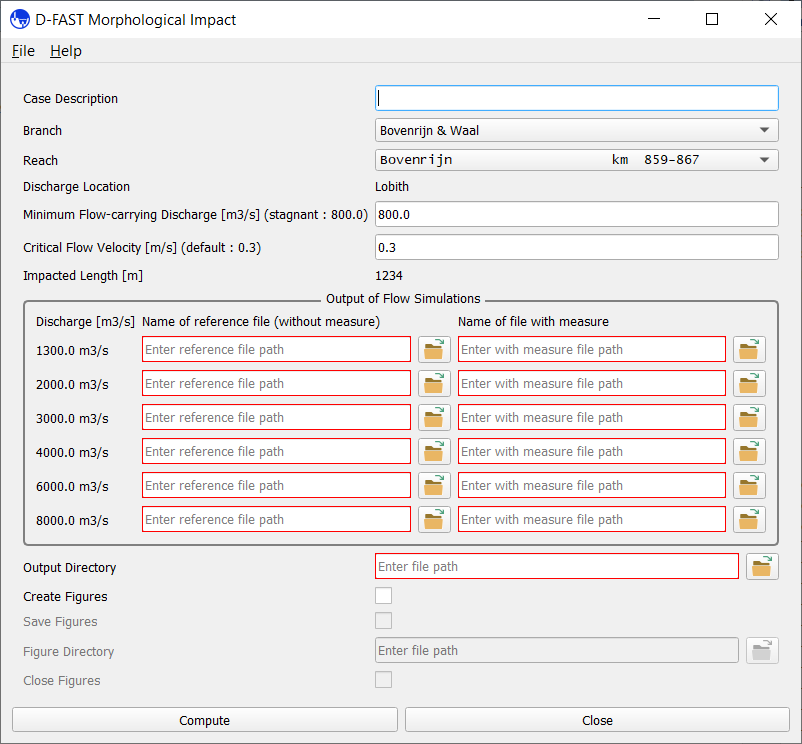
\includegraphics[width=12cm]{figures/main_dialog.png}
\caption{GUI after opening without configuration file}
\label{fig:test1.png}
\end{figure}
\end{enumerate}

\subsection{Test 2: save default configuration file}
\begin{enumerate}
\item Start from Test 1.
\item Select \menu{File} \textrightarrow \menu{Save}, and save the configuration file in the work folder as \file{test2}.
\item Verify that a file \file{test2.cfg} has been created and that the content matches

\verbfilenobox[\scriptsize]{figures/test2.cfg}
\end{enumerate}

\subsection{Test 3: modify settings}
\begin{enumerate}
\item Start from Test 2.
\item Specify "Test 3" as the Case description
\item Select branch "Maas"
\item Verify that the selected reach switches to Grensmaas, that the discharge location switches to Borgharen, and the (rounded) impacted length becomes \SI{0}{\metre}.
\item Select reach "Grave-Lith"
\item Verify that the impacted length becomes \SI{65}{\metre}.
\item Set the minimum flow-carrying discharge to \SI{2100}{\metre\cubed\per\second}
\item Verify that the impacted length reduces to \SI{8}{\metre}, and that the entry boxes for all discharges less or equal to 2100 are greyed-out.
\item Select from the folder \file{tests/c01 - GendtseWaardNevengeul} included in the \dfmi source code repository, the files \file{reference-Q1\_map.nc} and \file{measure-Q1\_map.nc} for the \SI{2500.0}{\metre\cubed\per\second} condition, and \file{reference-Q2\_map.nc} and \file{measure-Q2\_map.nc} for the \SI{3200.0}{\metre\cubed\per\second} condition as shown in \autoref{fig:test3.png}.
\item Verify that the red outline of the edit fields turns grey when valid file names are specified.
\item Select the output directory as \file{d:\textbackslash}.
\item Verify that the red outline of the edit field turns grey to signal that an existing path is specified.
\item Check the create figures box.
\item Verify that the Save and Close figures check boxes are activated when the create figures box is checked.
\item Verify that the dialog matches the following figure
\begin{figure}[H]
\center
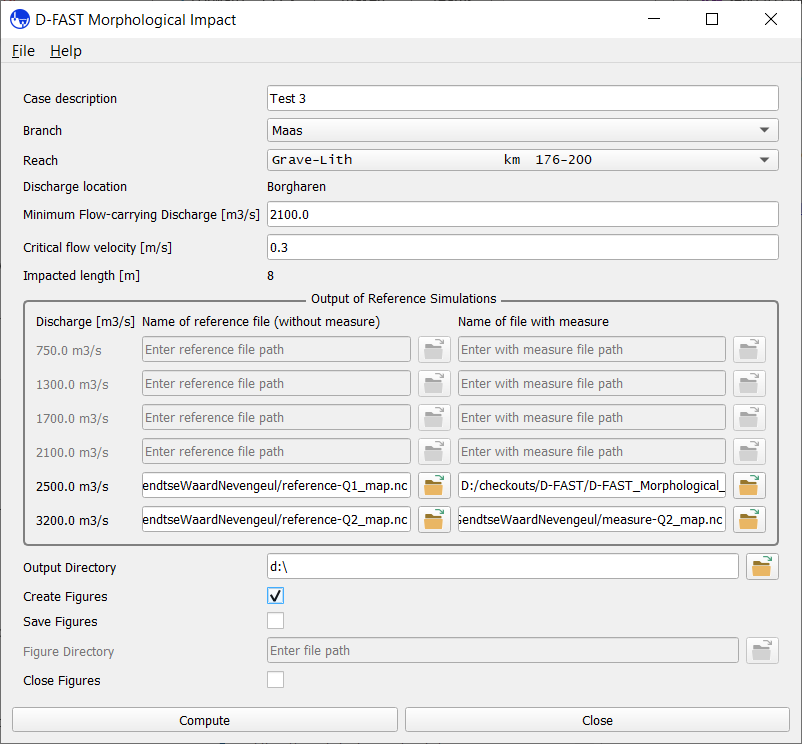
\includegraphics[width=12cm]{figures/test3.png}
\caption{GUI with edits}
\label{fig:test3.png}
\end{figure}
\end{enumerate}

\subsection{Test 4: save modified configuration file}
\begin{enumerate}
\item Start from Test 3.
\item Select \menu{File} \textrightarrow \menu{Save}, and save the configuration file in the work folder as \file{test4.cfg}.
\item Verify that a file \file{test4.cfg} has been created and that the content matches the following listing, but note that the relative paths may differ dependent on the work folder used

\verbfilenobox[\scriptsize]{figures/test4.cfg}
\end{enumerate}

\subsection{Test 5: load default configuration file}
\begin{enumerate}
\item Start from Test 4.
\item Select \menu{File} \textrightarrow \menu{Load}, and select the configuration file \file{test2.cfg}.
\item Verify that the dialog matches \autoref{fig:test1.png}.
\end{enumerate}

\subsection{Test 6: load modified configuration file}
\begin{enumerate}
\item Start from Test 5.
\item Select \menu{File} \textrightarrow \menu{Load}, and select the configuration file "test4.cfg".
\item Verify that the dialog matches \autoref{fig:test3.png}.
\end{enumerate}

\subsection{Test 7: view manual and about Windows}
\begin{enumerate}
\item Start from Test 6.
\item Select \menu{Help} \textrightarrow \menu{Open User Manual} and verify that the user manual is opened.
\item Select \menu{Help} \textrightarrow \menu{Version} and verify that the about box shown matches the image stored as "test7\_about.png" \autoref{fig:manual_system_test_7_about_dfastmi.png} except for the version number (which should match the version being tested) and the copyright year (which should match the year of the latest code update).
\begin{figure}[H]
	\center
	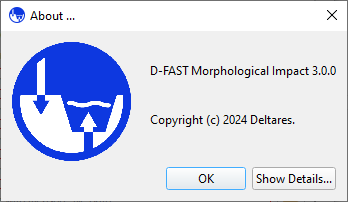
\includegraphics[width=8cm]{figures/manual_system_test_7_about_dfastmi.png}
	\caption{The \dfmi about box showing version and license information.}
	\label{fig:manual_system_test_7_about_dfastmi.png}
\end{figure}
\item Verify that pressing the \button{Show Details...} button reveal a text box stating "This software is distributed under the conditions of the GNU Lesser General Public License Version 2.1; see the LICENSE.md file for details."
\item Close the about box by pressing \button{OK}.
\item Select \menu{Help} \textrightarrow \menu{About Qt} and verify that the about box shown matches the image stored as "test7\_qt.png" \autoref{fig:manual_system_test_7_about_qt.png}.
\begin{figure}[H]
	\center
	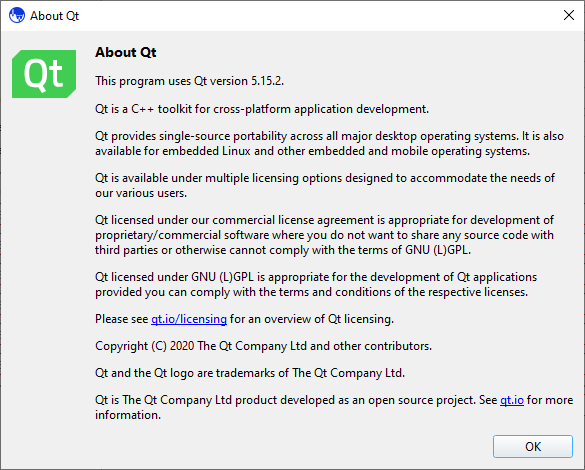
\includegraphics[width=12cm]{figures/manual_system_test_7_about_qt.png}
	\caption{The "About Qt" box.}
	\label{fig:manual_system_test_7_about_qt.png}
\end{figure}
\item Close the "About Qt" box by pressing \button{OK}.
\end{enumerate}

\subsection{Test 8: run \dflowfm analysis}
\begin{enumerate}
\item Start from Test 7.
\item Press the \button{Compute} button.
\item Verify that the analysis completes successfully.
\item The generated figure should correspond to \autoref{fig:report_Figure1.png}.
\item The content of the \file{report.txt} file in the output folder, should be equal to the following \hyperlink{code-report}{listing}.
\item Open the \file{dfastmi\_results.nc} file in QUICKPLOT.
Select the quantity "year-averaged bed level change without dredging" , and plot it using default settings.
See \autoref{fig:manual_system_test_8_quickplot_usage.png} for a snapshot of the steps in QUICKPLOT.
The resulting figure should correspond to \autoref{fig:report_Figure1_QP.png}.
\begin{figure}[H]
\center
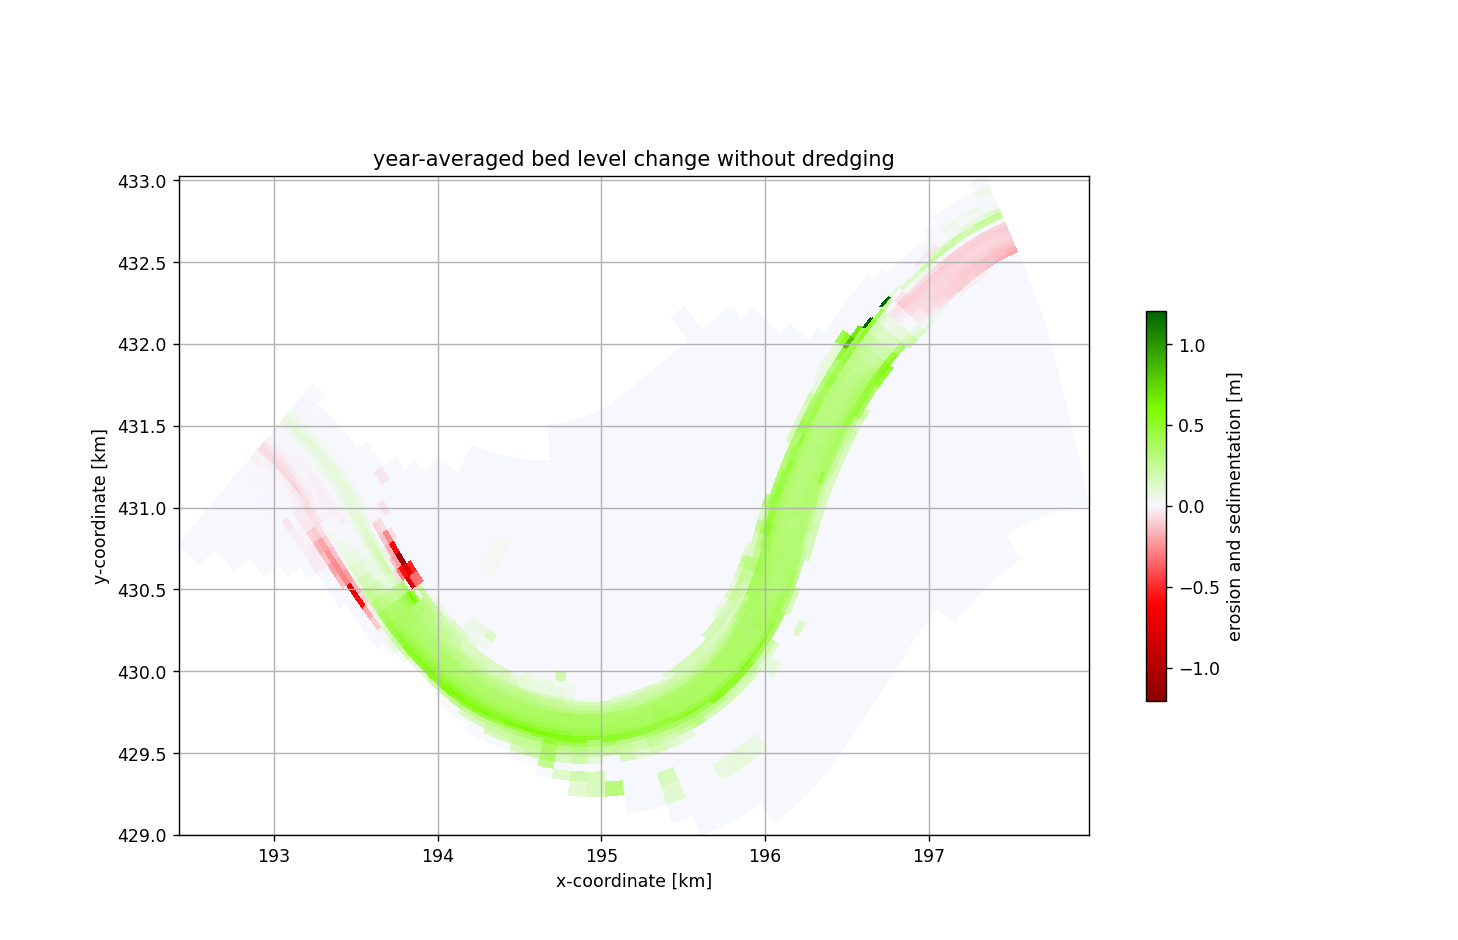
\includegraphics[width=12cm]{figures/report_Figure1.png}
\caption{Analysis results as plotted by \dfmi itself.}
\label{fig:report_Figure1.png}
\end{figure}
\end{enumerate}

\hypertarget{code-report}{\verbfilenobox[\scriptsize]{figures/report.txt}}

\begin{figure}[H]
	\center
	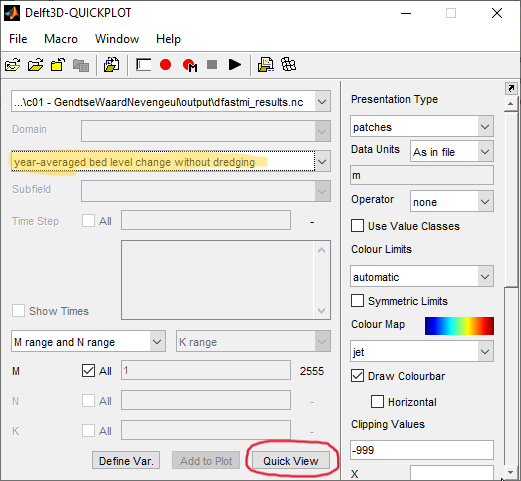
\includegraphics[width=12cm]{figures/manual_system_test_8_quickplot_usage.png}
	\caption{QUICKPLOT settings to create \autoref{fig:report_Figure1_QP.png}.}
	\label{fig:manual_system_test_8_quickplot_usage.png}
\end{figure}

\begin{figure}[H]
\center
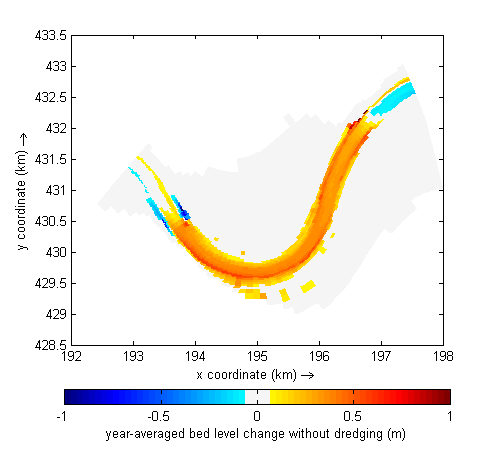
\includegraphics[width=12cm]{figures/report_Figure1_QP.png}
\caption{Analysis results as plotted using QUICKPLOT.}
\label{fig:report_Figure1_QP.png}
\end{figure}

\subsection{Test 9: closing the software}
\begin{enumerate}
\item Start from 8.
\item Close the program by one of the following methods:
\begin{itemize}
\item Select \menu{File} \textrightarrow \menu{Close}.
\item Press the \texttt{x} in the upper-right corner.
\item Press the \button{Close} button.
\end{itemize}
\item Reopen the program and test the other methods.
\item Verify that the program closes without any error using all methods.
\end{enumerate}

%-------------------------------
\chapter{Test Report} \label{Chp:TestReport}

The test plan describes (automated) regression tests, manual tests and the code quality checks.

\section{Manual tests}

This section summarizes the results of the manual testing of the graphical user interface.

\begin{tabular}{ll|l}
Test & Description & Success / Comments \\ \hline
1 & starting blank & OK \\
2 & save default configuration file & OK \\
3 & modify settings & OK \\
4 & save modified configuration file & OK \\
5 & load default configuration file & OK \\
6 & load modified configuration file & OK \\
7 & view manual and about Windows & OK \\
8 & run \dflowfm analysis & OK \\
9 & closing the software & OK \\
\end{tabular}


\section{Automated tests}

Below a brief pytest report of the automated regression testing is included below showing the number of source code lines per file, the number of lines \emph{not} covered by the source code testing phase and the resulting code coverage.
Note that the \keyw{\_\_main\_\_} module code is only executed in the binary testing phase.

\begin{Verbatim}
---------- coverage: platform win32, python 3.9.13-final-0 -----------
Name                                               Stmts   Miss  Cover
----------------------------------------------------------------------
dfastmi\__init__.py                                     4      0   100%
dfastmi\__main__.py                                    50     50     0%
dfastmi\batch\AFileNameRetriever.py                    12      0   100%
dfastmi\batch\AnalyserAndReporterDflowfm.py            16      0   100%
dfastmi\batch\AnalyserAndReporterWaqua.py              12      0   100%
dfastmi\batch\AnalyserDflowfm.py                      215     12    94%
dfastmi\batch\AnalyserWaqua.py                        150      1    99%
dfastmi\batch\AreaDetector.py                         108      0   100%
dfastmi\batch\AreaPlotter.py                           78      0   100%
dfastmi\batch\DFastUtils.py                            49     38    22%
dfastmi\batch\DflowfmReporters.py                      95     33    65%
dfastmi\batch\Distance.py                              54      6    89%
dfastmi\batch\Face.py                                  69      3    96%
dfastmi\batch\FileNameRetriever.py                     25      0   100%
dfastmi\batch\FileNameRetrieverFactory.py              22      0   100%
dfastmi\batch\FileNameRetrieverLegacy.py               14      0   100%
dfastmi\batch\FileNameRetrieverUnsupported.py           7      0   100%
dfastmi\batch\OutputDataDflowfm.py                     60      0   100%
dfastmi\batch\OutputDataWaqua.py                        9      0   100%
dfastmi\batch\PlotOptions.py                           81      3    96%
dfastmi\batch\Projection.py                            56     16    71%
dfastmi\batch\ReporterDflowfm.py                      108      0   100%
dfastmi\batch\ReporterWaqua.py                         20      0   100%
dfastmi\batch\SedimentationData.py                     11      0   100%
dfastmi\batch\SedimentationVolume.py                  125      3    98%
dfastmi\batch\XykmData.py                             115      1    99%
dfastmi\batch\XyzFileWriter.py                         15      0   100%
dfastmi\batch\core.py                                 211     12    94%
dfastmi\batch\plotting.py                             121     50    59%
dfastmi\cli.py                                        235     70    70%
dfastmi\cmd.py                                         28     28     0%
dfastmi\config\AConfigurationChecker.py                37      3    92%
dfastmi\config\AConfigurationInitializerBase.py        76      0   100%
dfastmi\config\ConfigFileOperations.py                127     16    87%
dfastmi\config\ConfigurationChecker.py                 59     11    81%
dfastmi\config\ConfigurationCheckerFactory.py          21      0   100%
dfastmi\config\ConfigurationCheckerLegacy.py           55      4    93%
dfastmi\config\ConfigurationCheckerValidator.py        13      0   100%
dfastmi\config\ConfigurationInitializer.py            104      5    95%
dfastmi\config\ConfigurationInitializerFactory.py      24      1    96%
dfastmi\config\ConfigurationInitializerLegacy.py       52      0   100%
dfastmi\gui\dialog_model.py                           140      1    99%
dfastmi\gui\dialog_utils.py                            56      0   100%
dfastmi\gui\dialog_view.py                            456     34    93%
dfastmi\gui\dialog_view_model.py                      162      4    98%
dfastmi\gui\qt_tools.py                                20      6    70%
dfastmi\io\AReach.py                                   20      0   100%
dfastmi\io\ApplicationSettingsHelper.py                43      0   100%
dfastmi\io\Branch.py                                   33      1    97%
dfastmi\io\CelerObject.py                              53      1    98%
dfastmi\io\ConfigBooleans.py                            2      0   100%
dfastmi\io\DFastAnalysisConfigFileParser.py            34      0   100%
dfastmi\io\DFastRiverConfigFileParser.py               87      0   100%
dfastmi\io\DataTextFileOperations.py                   65      1    98%
dfastmi\io\IBranch.py                                  16      0   100%
dfastmi\io\IReach.py                                   13      0   100%
dfastmi\io\ObservableList.py                           25      0   100%
dfastmi\io\Reach.py                                    48      0   100%
dfastmi\io\ReachLegacy.py                              11      0   100%
dfastmi\io\RiversObject.py                            120      2    98%
dfastmi\io\map_file.py                                138      3    98%
dfastmi\kernel\BedLevelCalculator.py                   60      0   100%
dfastmi\kernel\core.py                                 30      0   100%
dfastmi\kernel\legacy.py                               55      0   100%
dfastmi\kernel\typehints.py                             6      0   100%
dfastmi\resources.py                                    4      0   100%
-----------------------------------------------------------------------
TOTAL                                                4440    419    91%

====================== 455 passed, 33 warnings in 39.77s ======================
\end{Verbatim}

\section{Code check}
The quality of the \dfastmi source code and the code coverage is tracked by \href{https://sonarcloud.io/project/overview?id=Deltares_D-FAST_Morphological_Impact}{SonarCloud} and \href{https://sigrid-says.com/deltares/dfast-mi/-/overview}{Sigrid}.

\subsection{SonarCloud reports}
During the development of D-FAST MI 3.0.0, the number of code lines has doubled.
There is no duplication in the code anymore, see \autoref{fig:code_duplication}.
At the time of the first upload about 40\% of the code was covered by a limited set of about 65 tests.
The code coverage was still relatively high due to a few system tests that touched a lot of lines of code.
Since that time, the code coverage has increased to 90\% whereas at the same time the number of code lines has increased from about 2700 to almost 4400.
See \autoref{fig:code_coverage}.
During the same period the number of code issues detected by SonarCloud has decreased from 240 to 65.
Out of the remaining 65 issues, 15 are considered high severity, 20 medium severity and 30 low severity.
The 15 most critical issues are related to code complexity that is slightly too high, and \keyw{try-except} constructs that don't filter the exceptions that they catch.
See \autoref{fig:code_issues}.

\begin{figure}
\center
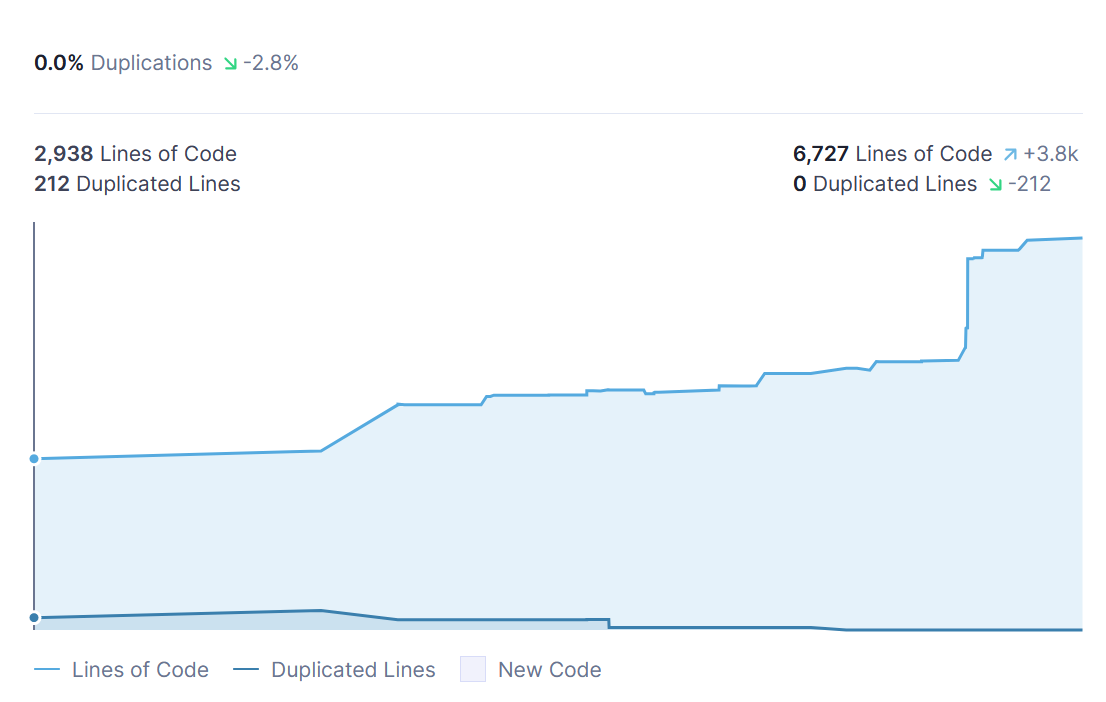
\includegraphics[width=10cm]{figures/code_duplication.png}
\caption{Code duplication}
\label{fig:code_duplication}
\end{figure}

\begin{figure}
\center
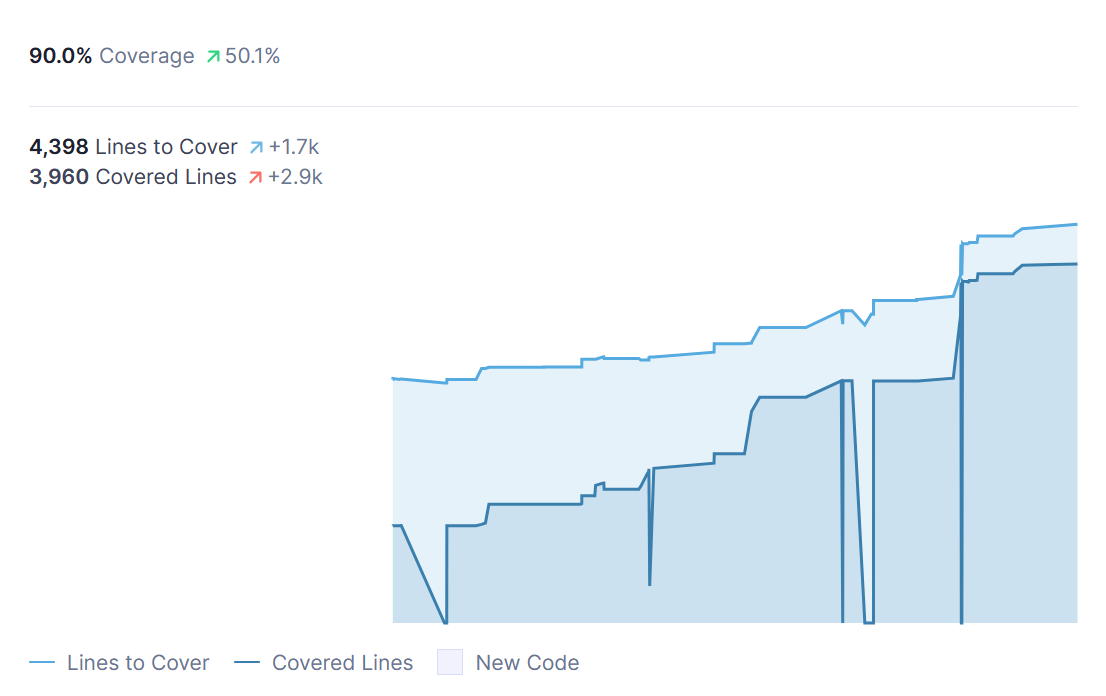
\includegraphics[width=10cm]{figures/code_coverage.png}
\caption{Code coverage}
\label{fig:code_coverage}
\end{figure}

\begin{figure}
\center
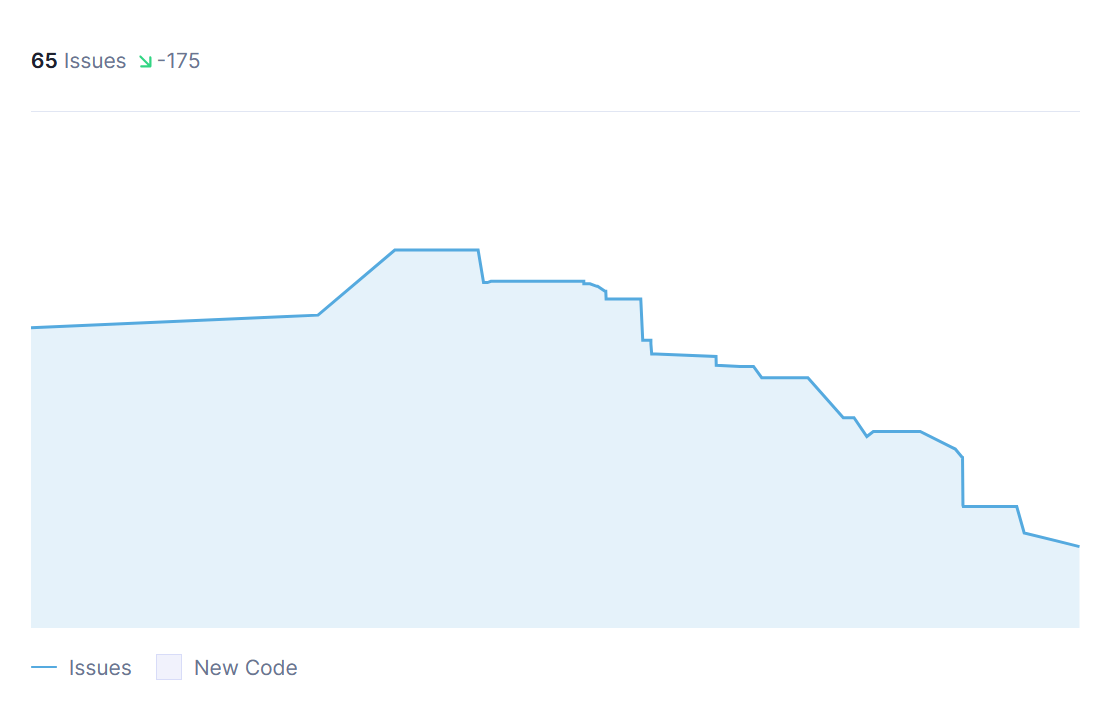
\includegraphics[width=10cm]{figures/code_issues.png}
\caption{Number of code issues flagged by SonarCloud}
\label{fig:code_issues}
\end{figure}

\subsection{Sigrid report}
The overall maintainability is scored at 3.6, with an architecture score of 3.4.
The total amount of code represents 11 person months (to develop).
The number of lines of code for testing is almost the same as the number of lines of code for the program itself (test/code ration = 92 \%).
The code depends on 60 open source libraries of which 5 (cftime, click-plugins, intel-openmp, mkl, tbb) are marked as high risk since the version used is more than 1 year old.
There is 1 critical security issue.
This is related to the opening the user manual by starting a shell process; someone might exploit this by starting some other process.

\begin{figure}
\center
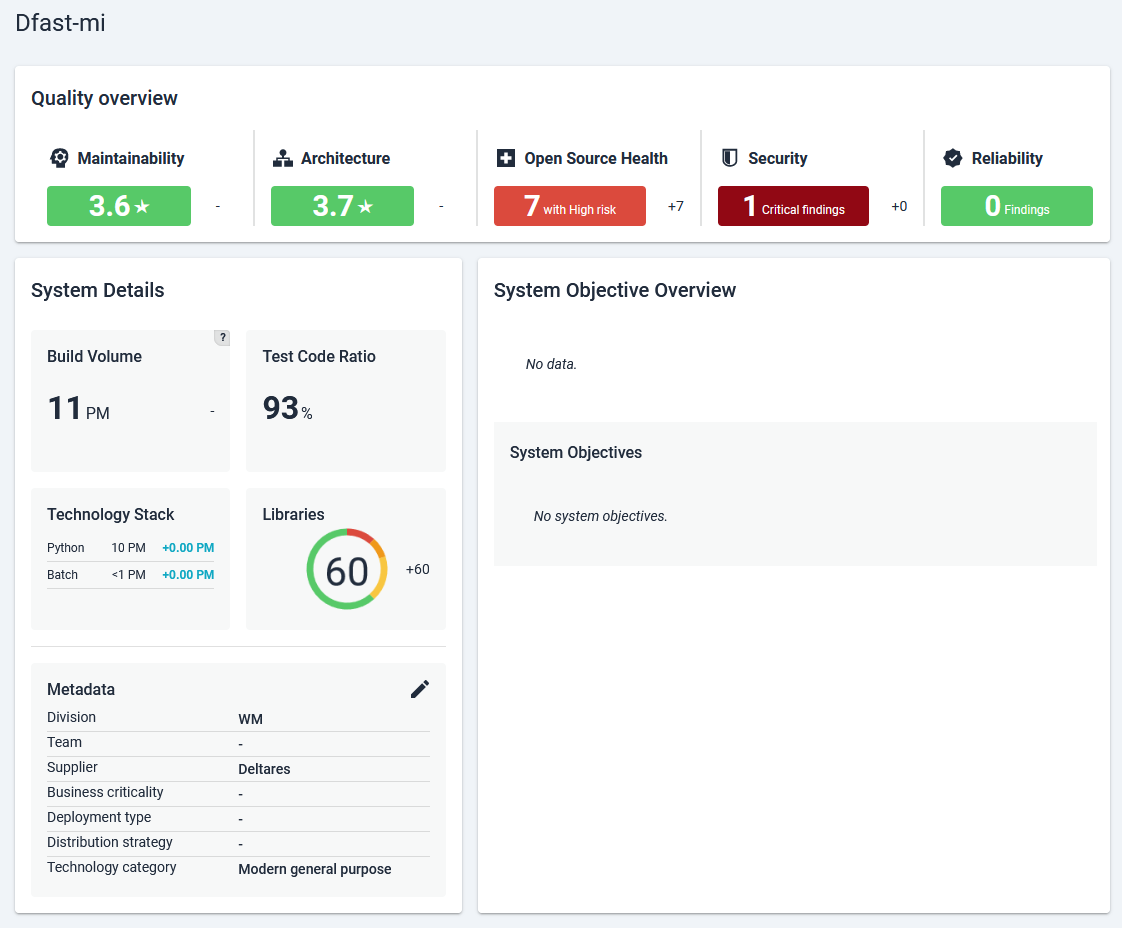
\includegraphics[width=\textwidth]{figures/sigrid.png}
\caption{Sigrid Overview}
\label{fig:sigrid_overview}
\end{figure}

\begin{figure}
\center
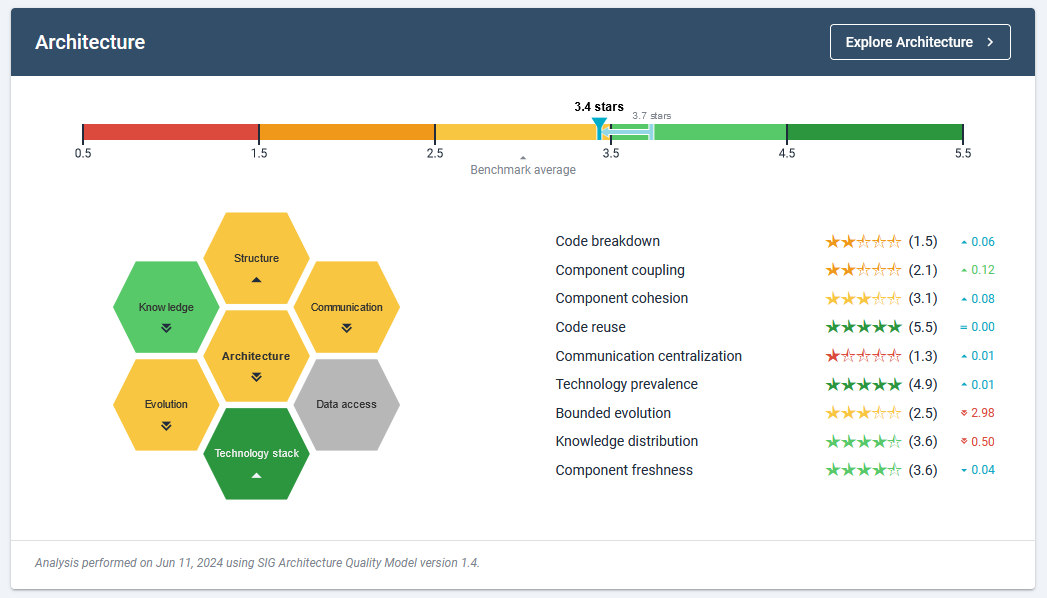
\includegraphics[width=\textwidth]{figures/sigrid-architecture.png}
\caption{Sigrid summary of architecture aspects}
\label{fig:sigrid_architecture_overview}
\end{figure}

\begin{figure}
\center
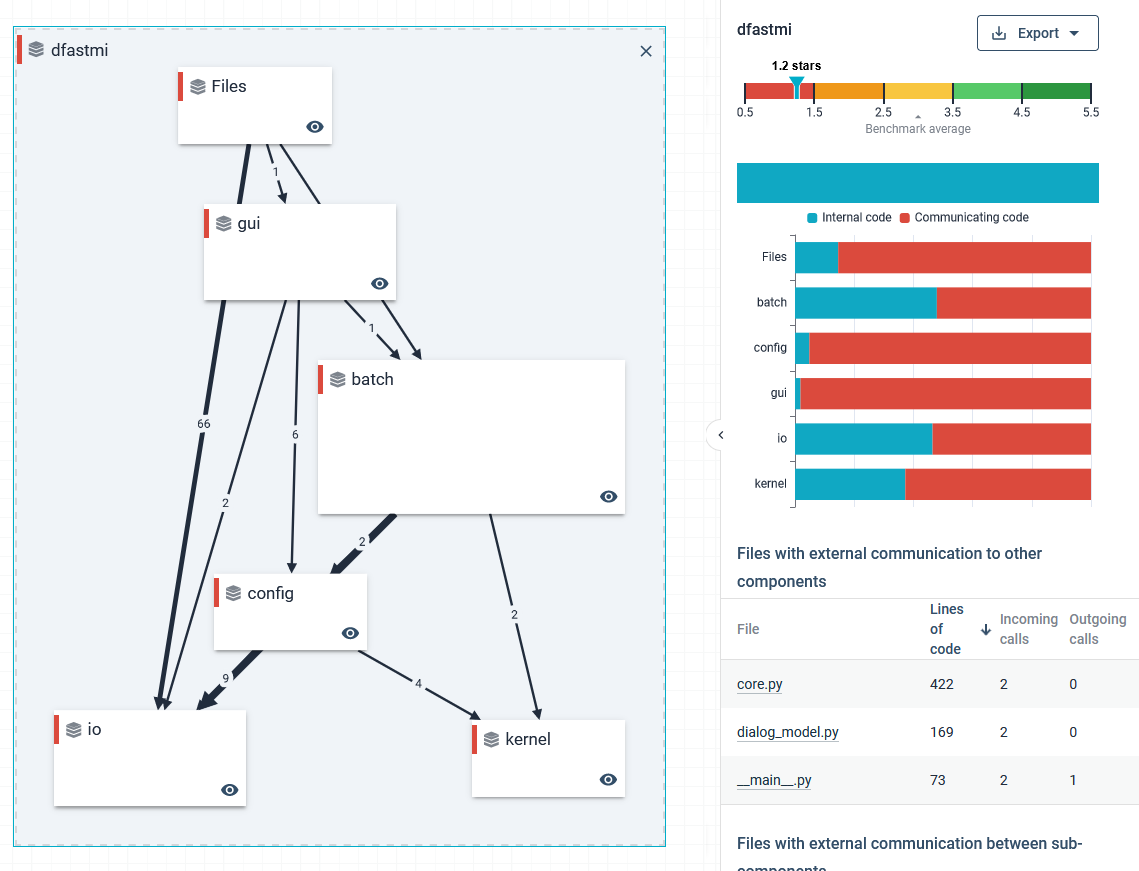
\includegraphics[width=\textwidth]{figures/sigrid-arch-communication.png}
\caption{Sigrid evaluation of communication centralization}
\label{fig:sigrid_architecture_comm}
\end{figure}

%\markdownInput{techref.md}

\nonumchapter{References}
\bibliography{dfastmi}

\appendix
\chapter{File formats}

The software distinguishes 6 files:

\begin{itemize}
\item The \emph{rivers configuration file} defines the branches and reaches, and all parameter settings specific for the overall system, per branch or per reach.
\item The \emph{dialog text file} defines all strings to be used in the interaction with the users (GUI, report, or error messages).
\item The \emph{analysis configuration file} defines the settings that are relevant for a specific execution of the algorithm, i.e.~for a specific branch, reach and intervention.
\item The \emph{simulation result files} define the spatial variations in the velocities and water depths as needed by the algorithm.
\item The \emph{report file} contains a logging of the settings and lumped results for the analysis.
\item The \emph{spatial output file} contains the estimate of the spatial variation in the sedimentation and erosion patterns that will result from the intervention (minimum, mean and maximum).
\end{itemize}

Each file type is addressed separately in the following subsections.

\section{Rivers configuration file}

The rivers configuration file follows the common ini-file format.
The file must contain a \keyw{[General]} block with a keyword \keyw{Version} to indicate the version number of the file.
The version number should be \keyw{3.0}.\footnote{Initially this file version was named \keyw{2.0} but to avoid confusion with the fact that this file format is only supported by \dfastmi version 3.0, the version number has been increased.
Files with version \keyw{2.0} are still accepted, but not recommended.}

Besides the \keyw{[General]} block version 3.0 files should only contain data blocks identifying the river branches (in Dutch: takken).
The names of those blocks will be used as branch names.
For instance, a block [My branch] will be processed as a branch called "My branch".
The order of the branches in the gui will correspond to the order of the blocks in the file.
The branch block defines the reaches (in Dutch: stukken) to be distinguished as well as the branch or reach specific parameter settings.
The \keyw{[General]} block may contain default values for the various parameters.
Further details follow below.

\begin{longtable}{l|l|p{8cm}}
\caption{Description of rivers configuration version 3} \\
Block & Keyword & Description \\ \hline
\endfirsthead
\multicolumn{3}{l}{\textsl{(continued from previous page)}} \\
Block & Keyword & Description \\ \hline
\endhead
\hline \multicolumn{3}{r}{\textsl{(continued on next page)}} \\
\endfoot
\endlastfoot
\keyw{General} & \keyw{Version} & Version number.
Should be \keyw{3.0}. \\
\keyw{General} & \keyw{checksum} & Checksum of the rivers configuration file.
Used to verify that the rivers configuration file wasn't accidentally modified. \\
BranchName<i> & \keyw{QLocation} & Location at which discharges for branch <i> are defined. \\
BranchName<i> & \keyw{Reach<j>} & Name of reach <j> within branch <i>. \\
\keyw{*} & \keyw{NWidth} & Normal width \unitbrackets{m} of main channel. \\
\keyw{*} & \keyw{QStagnant} & Discharge \unitbrackets{m\textsuperscript{3}/s} below which main channel flow can be assumed stagnant. \\
\keyw{*} & \keyw{UCrit} & Critical (minimum) velocity \unitbrackets{m/s} for sediment transport. \\

\keyw{*} & \keyw{HydroQ} & Series of discharges \unitbrackets{\SI{}{\metre\cubed\per\second}} representing each stage of the ``hydrograph''. \\
\keyw{*} & \keyw{Tide} & Flag to indicate whether the stages of the ``hydrograph'' are represented by discharge only (False) or by a combination of discharge and tide (True). \\
\keyw{*} & \keyw{TideBC} & Series of other tidal conditions representing the stages of the ``hydrograph''.
Only used in case \keyw{Tide} equals True. \\

\keyw{*} & \keyw{AutoTime} & Flag to indicate whether the duration of each discharge period should automatically be derived from the exceedance curve given by \keyw{QFit}.
The default value is False. \\
\keyw{*} & \keyw{HydroT} & Series of values specifying the duration of each stage of the ``hydrograph''.
The unit used for specifying the durations is arbitrary: the sum of all durations is assumed to be equivalent to 1 year.
The length of the series should be equal to the length of the series of discharges specified for \keyw{HydroQ}.
Only used in case \keyw{AutoTime} equals False. \\
\keyw{*} & \keyw{QFit} & Two discharges \unitbrackets{\SI{}{\metre\cubed\per\second}} used for representing the exceedance curve in case \keyw{AutoTime} equals True. \\

\keyw{*} & \keyw{CelerForm} & Flag to indicate the method used for determining the bed celerity.
The options are 1 (series of discharge, bed celerity pairs) and 2 (power-law relation between celerity and discharge).
The default value is 2. \\
\keyw{*} & \keyw{PropQ} & Strictly-monotonous increasing list of discharges \unitbrackets{\SI{}{\metre\cubed\per\second}} for which the bed celerity is given.
Only used in case \keyw{CelerForm} equals 1. \\
\keyw{*} & \keyw{PropC} & List of bed celerities \unitbrackets{\SI{}{\metre\per\second}} one value for each discharge specified by \keyw{PropQ}.
The length of the lists given by \keyw{PropQ} and \keyw{PropC} should be equal.
Only used in case \keyw{CelerForm} equals 1. \\
\keyw{*} & \keyw{CelerQ} & Two values representing the multiplication scalar and exponent of the power-law relation of the bed celerity \unitbrackets{\SI{}{\metre\per\second}} as function of the discharge \unitbrackets{\SI{}{\metre\cubed\per\second}}.
Only used in case \keyw{CelerForm} equals 2.
\end{longtable}

All keywords listed for block \keyw{*} may occur either in the \keyw{[General]} block or in one of the branch specific blocks where they may optionally be concatenated with the reach number <j>.
Those keywords may thus occur in three flavours:

\begin{enumerate}
\item Plain keyword in block \keyw{[General]}: global default value valid for all branches
\item Plain keyword in branch specific block: default value for that branch (overrules any global default)
\item Keyword followed by reach number <j> in branch specific block: value valid for that specific reach (on that branch).
\end{enumerate}

\subsubsection*{Example}

The following excerpt of the default \keyw{Dutch\_rivers.ini} configuration file shows the \keyw{[General]} as well as the first part of the \keyw{[Bovenrijn \& Waal]} block for the first branch.
It includes a global value of 0.3 for \keyw{UCrit} and 100 for \keyw{QMin}.
The other parameters are specified at branch level and mostly uniform for the whole branch.
Only \keyw{NWidth} and \keyw{PRLow} vary depending on the reach selected.

\begin{Verbatim}
    [General]
        Version    = 3.0
        UCrit      = 0.3
        CelerForm  = 1
        checksum   = 2377805458
    
    [Bovenrijn & Waal]
        QLocation  = Lobith
        HydroQ     = 1300 2000 3000 4000 6000 8000
        AutoTime   = True
        QStagnant  = 800
        QFit       = 800  1280
    
        Reach1     = Bovenrijn                    km  859-867
        NWidth1    = 340
        PropQ1     = 3500  3501
        PropC1     = 0.89  3.65
    
        Reach2     = Boven-Waal                   km  868-886
        NWidth2    = 260
        PropQ2     = 3500  3501
        PropC2     = 0.81  3.65

        ... continued ...
\end{Verbatim}

\section{Dialog text file}

The dialog text file uses the block labels enclosed by square brackets of the common ini-file format, but the lines in between the blocks are treated verbatim and don't list keyword/value pairs.
Every print statement in the program is associated with a short descriptive identifier.
These identifiers show up in the dialog text file as the block labels.
The text that follows the block label will be used at that location in the program.
The order of the blocks in the file is not important.
Please note that every line is used as is, so don't add indentations or blank lines unless you want those to show up during the program execution.
Most blocks may contain any number of lines, but some blocks may only contain a single line in particular block that start with \keyw{gui\_} or \keyw{filename\_}.
Some data blocks may contain one or more named placeholders, e.g. \keyw{{version}}, used for inserting values by means of the Python \keyw{format()} method.

\subsubsection*{Example}

The following excerpt of the default \keyw{messages.NL.cfg} dialog text file shows the string definition for 5 identifiers, namely '' (the identifier for an empty line), 'header', 'confirm', 'confirm\_or' and 'confirm\_or\_restart'.
The header string contains one placeholder, namely \keyw{{version}} for the the version number.

\begin{Verbatim}
    []
    
    [reduce_output]
    The option 'reduce_output' is active.
    
    [header]
    D-FAST Morphological Impact implements an algorithm to estimate the local
    morphological effects of a local intervention (i.e. an adjustment to the
    river). The conceptual framework was originally introduced in
        "RWS-WD memo WAQUA vuistregel 20-10-08"
    but it has been extended and improved over the years. Check the user manual
    for the details of the currently implemented algorithm.
    
    It is based on an estimation of the equilibrium bed level changes in the main
    channel that would occur eventually when river maintenance would not be
    adjusted.
    
    The effect is expressed as:
    
        year-averaged bed level change [m] without dredging
        maximum bed level change [m] without dredging
        minimum bed level change [m] without dredging
    
    By means of these estimates bottlenecks can be identified. The results are not
    suitable for direct estimation of the impact on the maintenance of the
    navigation channel!
    
    The combination of the total equilibrium sedimentation volume and the yearly
    sediment load of the river determines the period over which the equilibrium
    can be reached.
    
    
    This is version {version}.
    
    [confirm]
    Confirm using "y" ...
    
    [confirm_or]
    Confirm using "y", or reply "n" ...
    
    ... continued ...
\end{Verbatim}

\section{Analysis configuration file}\label{app:config}

The analysis configuration file follows the common ini-file format.
The file must contain a \keyw{[General]} block with a keyword \keyw{Version} to indicate the version number of the file.
The version number should be \keyw{3.0}.\footnote{Initially this file version was named \keyw{2.0} but to avoid confusion with the fact that this file format is only supported by \dfastmi version 3.0, the version number has been increased.
Files with version \keyw{2.0} are still accepted, but not recommended.}

Version 3.0 files must contain in the \keyw{[General]} block also the keywords \keyw{Branch} and \keyw{Reach} to identify the branch (in Dutch: tak) and reach (in Dutch: stuk) in which the intervention is located.
The specified names may be shortened, but they should uniquely identify the branch and reach amongst the names of the other branches and reaches.
The same block may also contain \keyw{QThreshold} and \keyw{UCrit} values representative for this particular intervention if they differ from those typical for the selected reach.
Furthermore, this block may contain \keyw{FigureDir} and \keyw{OutputDir} specifying where the figures and other output files should be written.
The \keyw{RiverKM} keyword to specify the chainage along the reach of interest is needed for estimating the initial year dredging volumes.
Last but not least, the user needs to specify the names of the D-Flow FM map- or fourier-files containing the results of the simulations without intervention (reference) and with intervention for the selected flow conditions.
These names must be specified in a continuous sequences of numbered blocks named \keyw{C1}, \keyw{C2}, etc.
The order of the blocks is not important: the relevant blocks are identified by means of the \keyw{Discharge} and optionally \keyw{TideBC} specified per block.
There should be a match for every stage of the configured ``hydrograph'' for the selected branch/reach.
The file names may be specified using relative or absolute paths.

\begin{tabular}{l|l|p{8cm}}
Block & Keyword & Description \\ \hline
\keyw{General} & \keyw{Version} & Version number.
Should be \keyw{3.0}. \\
\keyw{General} & \keyw{CaseDescription} & Description of the analysis. \\
\keyw{General} & \keyw{Branch} & Name of the selected branch. \\
\keyw{General} & \keyw{Reach} & Name of the selected reach. \\
\keyw{General} & \keyw{QThreshold} & Minimum discharge \unitbrackets{\SI{}{\metre\cubed\per\second}} at which intervention becomes active. \\
\keyw{General} & \keyw{UCrit} & Critical (minimum) velocity \unitbrackets{\SI{}{\metre\per\second}} for sediment transport. \\
\keyw{General} & \keyw{RiverKM} & Name of file with river chainage \unitbrackets{\SI{}{\kilo\metre}} and corresponding xy-coordinates. \\
\keyw{General} & \keyw{FigureDir} & Directory for storing figures (default relative to work dir: figure). \\
\keyw{General} & \keyw{OutputDir} & Directory for storing output files. \\
\keyw{C}<i> & \keyw{Discharge} & Discharge \unitbrackets{m\textsuperscript{3}/s} of condition <i>. \\
\keyw{C}<i> & \keyw{TideBC} & Tidal boundary of condition <i>. \\
\keyw{C}<i> & \keyw{Reference} & Name of D-Flow FM map- or fourier-file to be used for reference condition <i>. \\
\keyw{C}<i> & \keyw{WithIntervention} & Name of D-Flow FM map- or fourier-file that includes the intervention <i>. \\
\end{tabular}

\subsubsection*{Example}

This example shows a complete analysis configuration file for an intervention in the first branch/reach of the default \keyw{Dutch\_rivers.cfg} configuration.
It reports the default settings.
Only the \keyw{Version}, \keyw{Branch}, \keyw{Reach}, \keyw{Reference} and \keyw{WithIntervention} keywords are required for the full analysis.

\begin{Verbatim}
    [General]
      Version          = 3.0
      CaseDescription  = 
      Branch           = Bovenrijn & Waal
      Reach            = Boven-Waal                   km  868-886
      Qthreshold       = 1000.0
      Ucrit            = 0.3
      OutputDir        = 
      Plotting         = False
      SavePlots        = False
      FigureDir        = 
      ClosePlots       = False
      RiverKM          = 
    
    [C1]
      Discharge        = 1300.0
      Reference        = Case42/Q1/Reference/DFM_OUTPUT_Q1/Q1_map.nc
      WithIntervention = Case42/Q1/Updated/DFM_OUTPUT_Q1/Q1_map.nc
    
    [C2]
      Discharge        = 2000.0
      Reference        = Case42/Q2/Reference/DFM_OUTPUT_Q2/Q2_map.nc
      WithIntervention = Case42/Q2/Updated/DFM_OUTPUT_Q2/Q2_map.nc
    
    [C3]
      Discharge        = 3000.0
      Reference        = Case42/Q3/Reference/DFM_OUTPUT_Q3/Q3_map.nc
      WithIntervention = Case42/Q3/Updated/DFM_OUTPUT_Q3/Q3_map.nc

        ... continued ...
\end{Verbatim}

\section{Simulation result files}

\dfastmi expects all data in UGRID netCDF file similar to the map-file output of \dflowfm.
\dfastmi reads the results directly no conversion is necessary.
These files may contain multiple time steps; the final time steps will be used for the analysis.
The mesh geometry is transferred from one of the simulation files to the \dfastmi spatial output "results" file.

\section{Report file}

\dfastmi will write a report of the analysis.
This report file is a simple text file consistent with the earlier reports written by WAQMORF.
The length and content of the report vary depending on the availability of the simulation result files and the language selected.


\section{Spatial output file}

\dfastmi generates one UGRID netCDF file containing the spatial results of the analysis.
The mesh information is copied from the first D-Flow FM map- or fourier-file read, and the three data fields (erosion and sedimentation patterns for mean, minimum, and maximum impact) follow standardized conventions for data stored at cell centres (\keyw{face}-values) on an unstructured mesh.
As a result the data may be visualized using a number of visualization tools such as QUICKPLOT and QGIS.

\chapter{Backward compatibility} \label{Chp:backward}

\dfastmi may be run in \keyw{cli} mode for backward compatible with WAQMORF: in this (legacy) mode the configuration for the analysis is obtained by asking the user questions via a command line interface which support simulation results from WAQUA only.
The input and output as well as the description of the conceptual framework of that version is described in this appendix.

\dfastmi can also be run in backward compatible \keyw{batch} mode by specifying version 1 files for the rivers configuration and analysis configuration.

\section{Running in interactive command line mode}

The cli mode runs an interactive command line analysis using WAQUA results; this run mode does not support \dflowfm files.
The program should be started with the run mode set to \keyw{cli} on the command line as follows

\begin{Verbatim}
> dfastmi --mode cli
\end{Verbatim}

You may choose to run the program in either Dutch \keyw{-{}-language NL} (like the original WAQMORF) or English \keyw{-{}-language UK}; the latter is the default.
Please note that the language not only affects the text in the report, but also the names of the output files as indicated in the opening section of this chapter.
You may also choose to select the \keyw{-{}-reduced\_output} option for smaller SIMONA BOX file output.
When the program is started in this way, the program will ask you questions on the command line.
An example of the dialog is given in \autoref{Sec:cli_dialog}.
Because the \dfmi binary distributed suppresses the DOS box, this backward compatibility option is currently not accessible interactively.
Although this run mode is designed as an interactive dialog, you may use this mode also as a batch mode by redirecting standard input to read from file as follows

\begin{Verbatim}
> dfastmi --mode cli < myfile.in
\end{Verbatim}

In this case each line in the file \file{myfile.in} should contain the appropriate answer to the question.
This run mode is included for backward compatibility and comparison with its predecessor WAQMORF.
It should not be used for new studies based on \dflowfm results.

\section{Output files}

The \emph{cli mode} produces the following four output files:

\begin{itemize}
\item Text file with summary report of the analysis \\
English: \keyw{report.txt} \\
Dutch: \keyw{verslag.run}
\item Average yearly change in SIMONA BOX file format (when the analysis runs using WAQUA input) \\
English: \keyw{yearavg\_dzb.out} \\
Dutch: \keyw{jaargem.out}
\item Maximum change in SIMONA BOX file format (when the analysis runs using WAQUA input) \\
English: \keyw{max\_dzb.out} \\
Dutch: \keyw{maxmorf.out}
\item Minimum change in SIMONA BOX file format (when the analysis runs using WAQUA input) \\
English: \keyw{min\_dzb.out} \\
Dutch: \keyw{minmorf.out}
\end{itemize}

\section{Conceptual framework}

This section describes the conceptual framework of the method used by \dfastmi version 2, and by version 3 in backward compatibility mode, and the derivation of the river parameters used for the Dutch rivers.

\subsection{Characteristics of bed level changes due to river interventions}

A river intervention, i.e.~a local river adjustment (typically a flow capacity enlarging adjustment) outside the main channel, may result in changes in the flow pattern within the main channel.
The bed levels within the main channel will react to such changes depending on the

\hspace{1cm}\emph{magnitude, duration and length scale of these flow pattern changes in the main channel.}

Hence, the core focus of the rule-of-thumb is to determine and characterize the changes in the flow pattern within the main channel.
Here, we define the main channel as the part of the river between the groyne heads.

At the upstream end of the floodplain adjustment part of the main channel discharge will leave the main channel, which will flow through the enlarged floodplain, secondary channel or bank area, and return to the main channel at the downstream end of the project area.
The resulting changes in the main channel flow pattern cause sedimentation in the main channel at the upstream "offtake" of the new outflow and erosion at the downstream "confluence" when the flow enters the main channel again.
Because the river discharge varies, the pattern will also vary during the year
As a result a part of the main channel bed level adjustment is stationary and a part of the adjustment is transitional and it will migrate downstream.
A reduction in the water depth may thus not only be observed locally where the flow diverges into the flood plain, but also downstream thereof.

The bed level change due to river enlargement can largely be characterized as follows

\begin{itemize}
\item The magnitude of the bed level change varies over the seasons; the maximum change is observed at the end of the flood season and the adjustment reaches a minimum at the end of the low flow period.

\item Local evaluation of the bed level changes is insufficient because of partial downstream migration of the bed level changes.

\item The maximum impact is observed on that side of the river which is closest to the adjustment.
\end{itemize}

Because part of the bed level changes migrate downstream, the morphological impact on projects located downstream may be increased.
After all, the maximum bed level change of one single river enlarging intervention is reached at the end of the flood period and it's the result of that flood period.
However, when a series of interventions along the river are combined (for instance, lowering of the groynes along a reach) the downstream bed level changes may be increased by accumulation of downstream migrating bed waves, such that the accumulated bed level change may be significantly larger.
In other words, river interventions extending over longer reaches may result in a larger morphodynamic response than comparable but more isolated interventions.

The aforementioned observations result in the following premises.
The rule-of-thumb described in the following sections

\begin{itemize}
\item will only be valid for the estimation of the impact of local interventions with a length of at most one flood plain,

\item should take into account seasonal variations, and

\item needs to be estimate the spatial pattern of the bed level change.
\end{itemize}


\subsection{Characterization of the changes in the main channel flow pattern}

When an intervention in the floodplains does not include something like a permanently active secondary channel, the flow pattern in the main channel will only be affected during flood conditions.
If on the other hand, such a secondary channel (or other intervention active under medium to low flow conditions such as groyne adjustments) is included in the design then the flow pattern will also be influenced during transitional or even low flow conditions.
It's therefore critical to determine the effect of the intervention on the main channel flow pattern at different discharge levels.

Secondary channels may have a major impact on the morphodynamics of the main channel.
The magnitude of the discharge through the secondary channel varies as function of the river discharge.
Because the hydraulic conditions of the secondary channel can change over time (e.g.~due to vegetation, siltation, or erosion) the discharge through a secondary channel is typically controlled by some hydraulic structure.
The typical characteristics of a weir (overlaat, drempel) and orifice (onderlaat, duiker) are shown in \autoref{App.Fig1}.

\begin{figure}
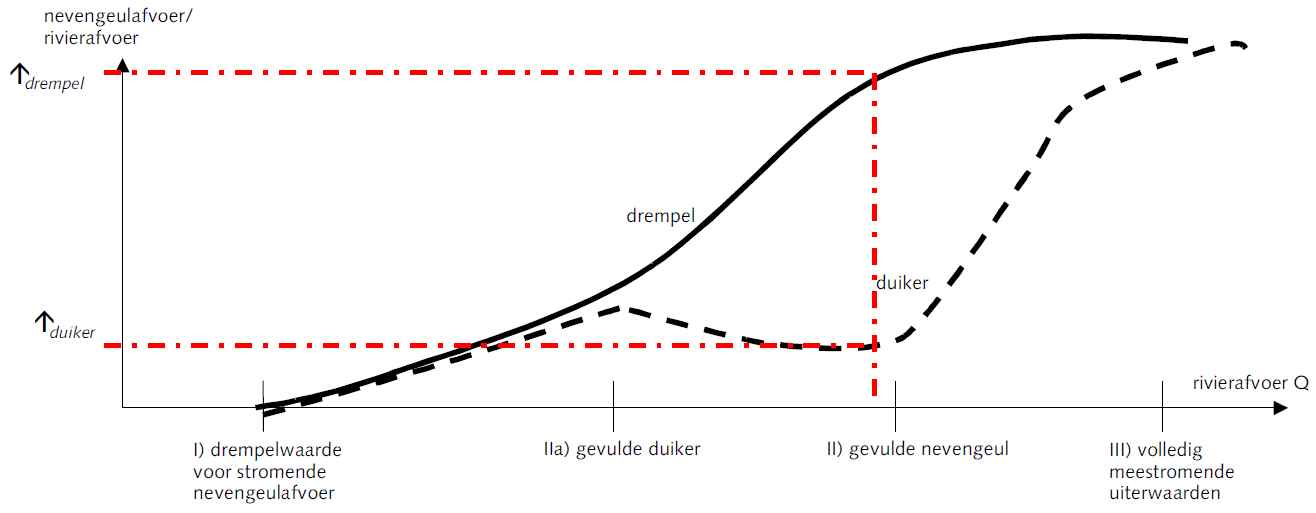
\includegraphics[width=\columnwidth]{figures/Fig1.png}
\caption{Schematic of the controlled discharge through a secondary channel.}
\label{App.Fig1}
\end{figure}

The discharge through a secondary channel is characterized by a number of special conditions as illustrated by \autoref{App.Fig1}:

\begin{enumerate}
\item the beginning of flow through the secondary channel
\item the bankfull secondary channel
\item the fully developed flow in the secondary channel and surrounding floodplain.
\end{enumerate}

When the discharge through the secondary channel is controlled by an orifice, the fully flooded condition may add an additional characteristic discharge.

In order to characterize the flow patterns during flood it's necessary to distinguish the condition in which the flood plains just start to carry flows, and the condition of fully developed flow in the flood plains.
Based on results of 1D simulations shown in \autoref{App.Fig2a} it has been concluded that for the Rhine branches a discharge of 6000 m\textsuperscript{3}/s at Lobith can be used as the boundary between those two conditions.
The flow through the bank zone (\autoref{App.Fig2b}) is also largely developed for discharges at Lobith larger than
6000 m\textsuperscript{3}/s.

\begin{figure}
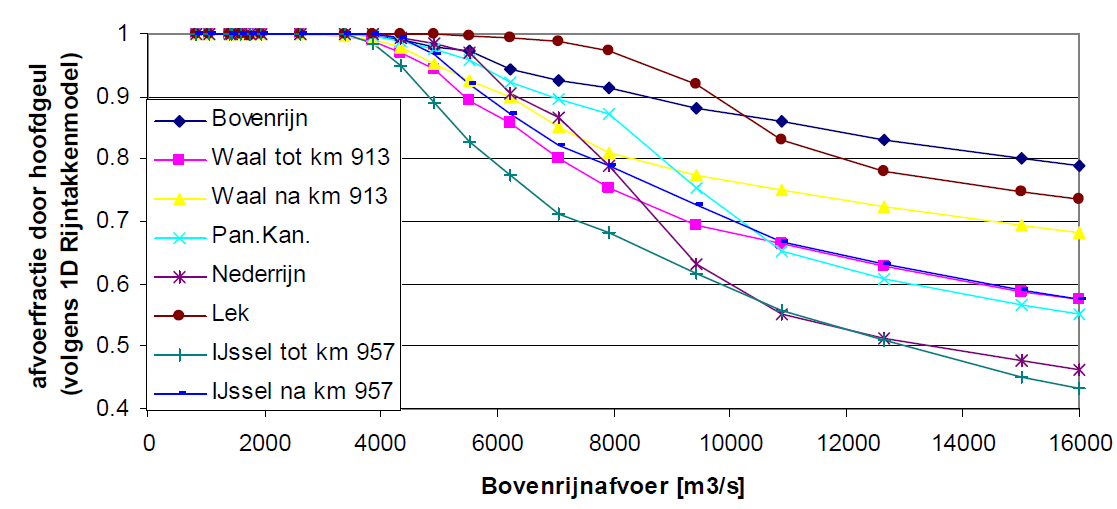
\includegraphics[width=\columnwidth]{figures/Fig2a.png}
\caption{Reach-averaged discharge fraction through the main channel (based on 1D model of the Rhine branches).}
\label{App.Fig2a}
\end{figure}

\begin{figure}
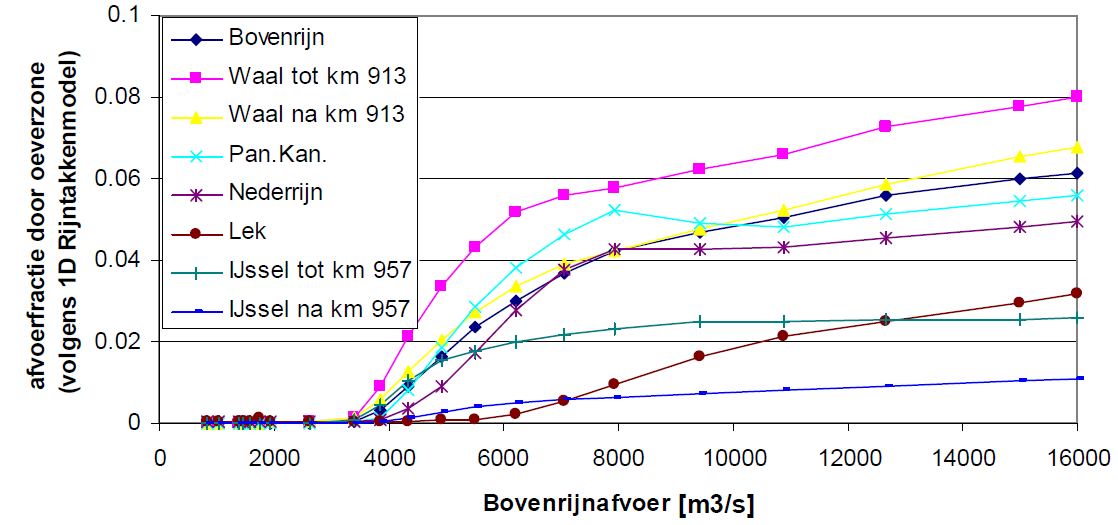
\includegraphics[width=\columnwidth]{figures/Fig2b.png}
\caption{Reach-averaged discharge fraction through the bank zone (based on 1D model of the Rhine branches).}
\label{App.Fig2b}
\end{figure}

These characteristic discharge values can be used to schematize the river hydrograph effectively by means of a limited number of discrete discharge conditions.
Three discharge blocks turn out to be sufficient for many interventions as may bed concluded from \autoref{App.Tab1}.
That is why it has been concluded that \emph{three flow conditions are sufficient to schematize the yearly hydrograph for the purpose of estimating the morphological impact of local interventions}.

\begin{table}
\small
%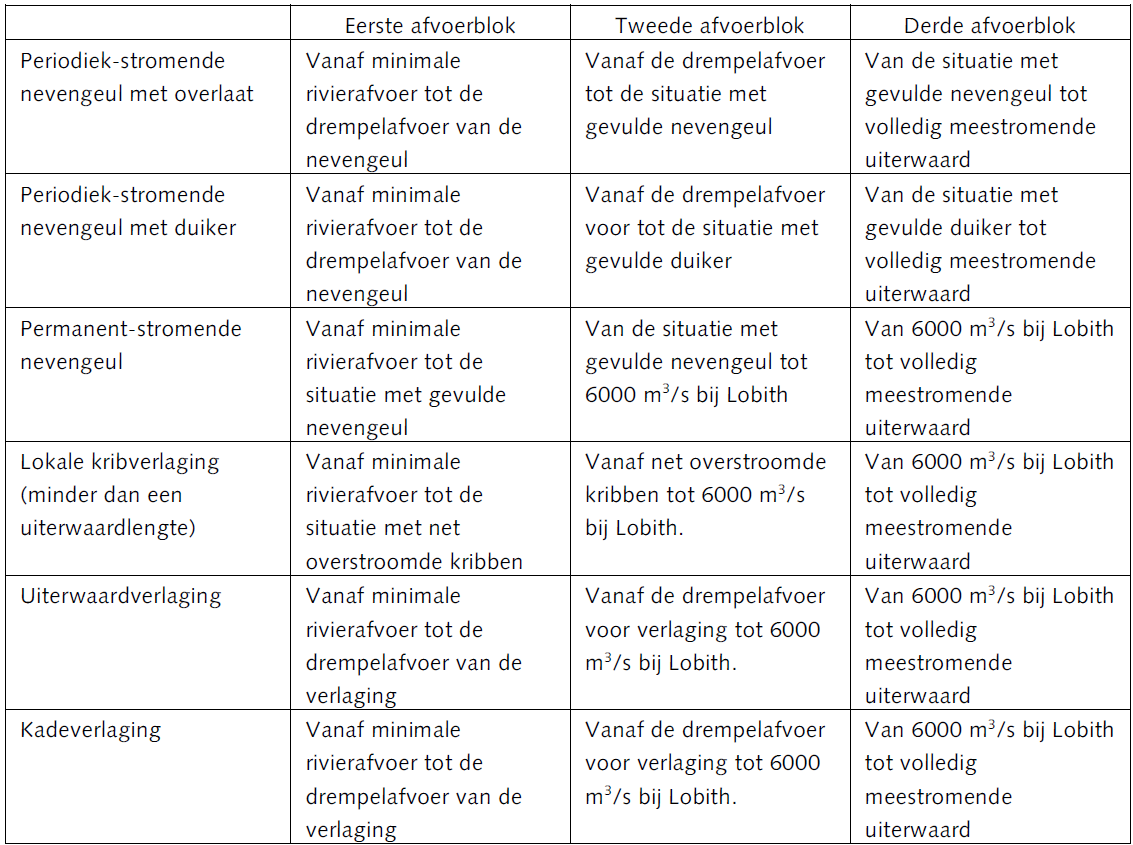
\includegraphics[width=\columnwidth]{figures/Tab1a.png}
\begin{tabular}{p{\columnwidth/4-12pt}|p{\columnwidth/4-12pt}|p{\columnwidth/4-12pt}|p{\columnwidth/4-12pt}}
 & first block & second block & third block \\ \hline
periodically flowing secondary channel with weir & from minimum river flow to minimum discharge for secondary channel & from minimum discharge for secondary channel to bankfull secondary channel & from bankfull secondary channel to fully developed flood plain flow \\ \hline
periodically flowing secondary channel with orifice & from minimum river flow to minimum discharge for secondary channel & from minimum discharge for secondary channel to fully flooded orifice & from fully flooded orifice to fully developed flood plain flow \\ \hline
permanently flowing secondary channel & from minimum river flow to bankfull secondary channel & from bankfull secondary channel to 6000 m\textsuperscript{3}/s at Lobith & from 6000 m\textsuperscript{3}/s at Lobith to fully developed flood plain flow \\ \hline
local lowering of groynes (less than flood plain length) & from minimum river flow to flooded groynes & from flooded groynes to 6000 m\textsuperscript{3}/s at Lobith & from 6000 m\textsuperscript{3}/s at Lobith to fully developed flood plain flow \\ \hline
lowering of the flood plain & from minimum river flow to minimum discharge for new flood plain threshold & from new flood plain threshold to 6000 m\textsuperscript{3}/s at Lobith & from 6000 m\textsuperscript{3}/s at Lobith to fully developed flood plain flow \\ \hline
lowering of levees & from minimum river flow to minimum discharge for new levee threshold & from new levee threshold to 6000 m\textsuperscript{3}/s at Lobith & from 6000 m\textsuperscript{3}/s at Lobith to fully developed flood plain flow \\
\end{tabular}

\caption{Overview of discharge conditions for various interventions in a free flowing Rhine branch.}
\label{App.Tab1}
\end{table}

For a river reach in which water levels (and hence flow conditions) are controlled by means of barriers for a period $T_\text{stuw}$, the minimum river discharge is determined by the river discharge at which the barriers are opened.
\autoref{App.Fig6} shows that the barriers in the Nederrijn are opened at a discharge of 1500 m\textsuperscript{3}/s in the Bovenrijn at Lobith (this value is exceeded during 57 \% of the year) and that the branch is approximately free flowing for discharges above 2200 m\textsuperscript{3}/s in the Bovenrijn at Lobith (exceeded during 33 \% of the year).

\begin{table}
%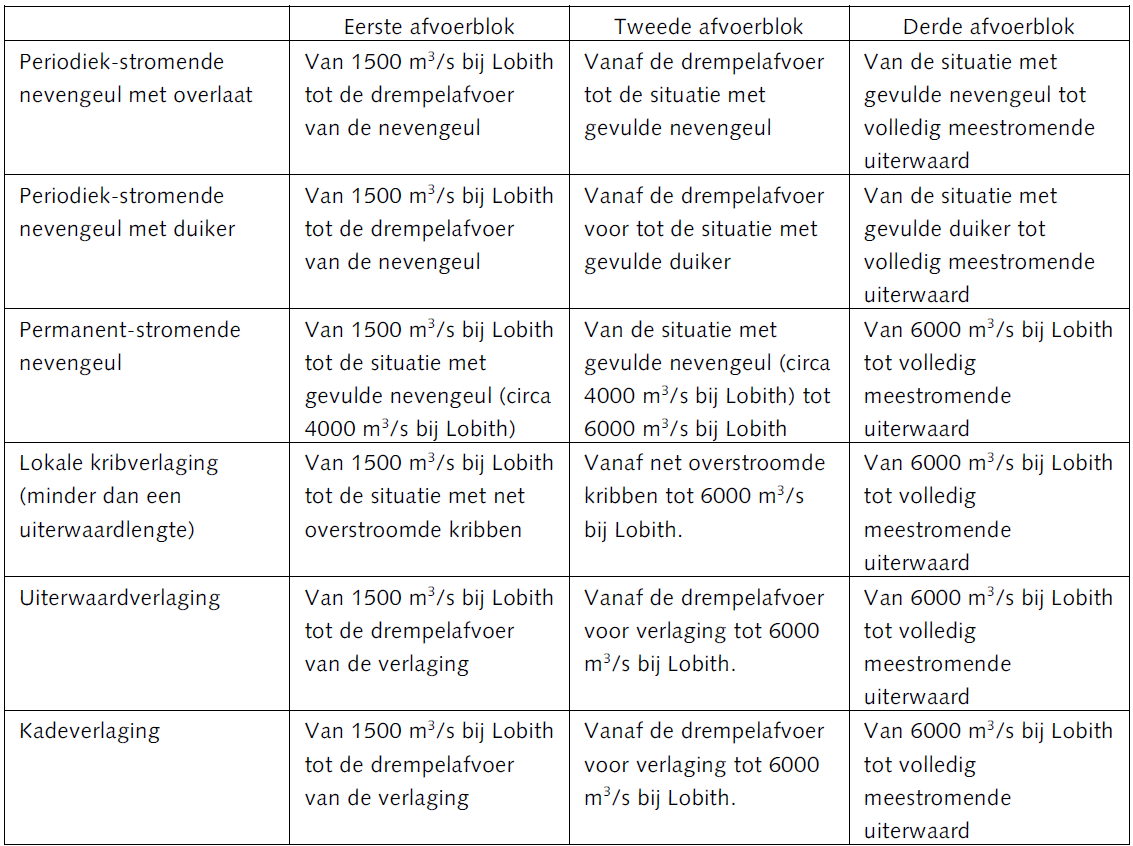
\includegraphics[width=\columnwidth]{figures/Tab1b.png}
\begin{tabular}{p{\columnwidth/4-12pt}|p{\columnwidth/4-12pt}|p{\columnwidth/4-12pt}|p{\columnwidth/4-12pt}}
 & first block & second block & third block \\ \hline
periodically flowing secondary channel with weir & from 1500 m\textsuperscript{3}/s at Lobith to minimum discharge for secondary channel & from minimum discharge for secondary channel to bankfull secondary channel & from bankfull secondary channel to fully developed flood plain flow \\ \hline
periodically flowing secondary channel with orifice & from 1500 m\textsuperscript{3}/s at Lobith to minimum discharge for secondary channel & from minimum discharge for secondary channel to fully flooded orifice & from fully flooded orifice to fully developed flood plain flow \\ \hline
permanently flowing secondary channel & from 1500 m\textsuperscript{3}/s at Lobith to bankfull secondary channel (about 4000 m\textsuperscript{3}/s at Lobith) & from bankfull secondary channel (about 4000 m\textsuperscript{3}/s at Lobith) to 6000 m\textsuperscript{3}/s at Lobith & from 6000 m\textsuperscript{3}/s at Lobith to fully developed flood plain flow \\ \hline
local lowering of groynes (less than flood plain length) & from 1500 m\textsuperscript{3}/s at Lobith to flooded groynes & from flooded groynes to 6000 m\textsuperscript{3}/s at Lobith & from 6000 m\textsuperscript{3}/s at Lobith to fully developed flood plain flow \\ \hline
lowering of the flood plain & from 1500 m\textsuperscript{3}/s at Lobith to minimum discharge for new flood plain threshold & from new flood plain threshold to 6000 m\textsuperscript{3}/s at Lobith & from 6000 m\textsuperscript{3}/s at Lobith to fully developed flood plain flow \\ \hline
lowering of levees & from 1500 m\textsuperscript{3}/s at Lobith to minimum discharge for new levee threshold & from new levee threshold to 6000 m\textsuperscript{3}/s at Lobith & from 6000 m\textsuperscript{3}/s at Lobith to fully developed flood plain flow \\
\end{tabular}

\caption{Overview of discharge conditions for various interventions along the Nederrijn.}
\label{App.Tab2}
\end{table}

\begin{table}
%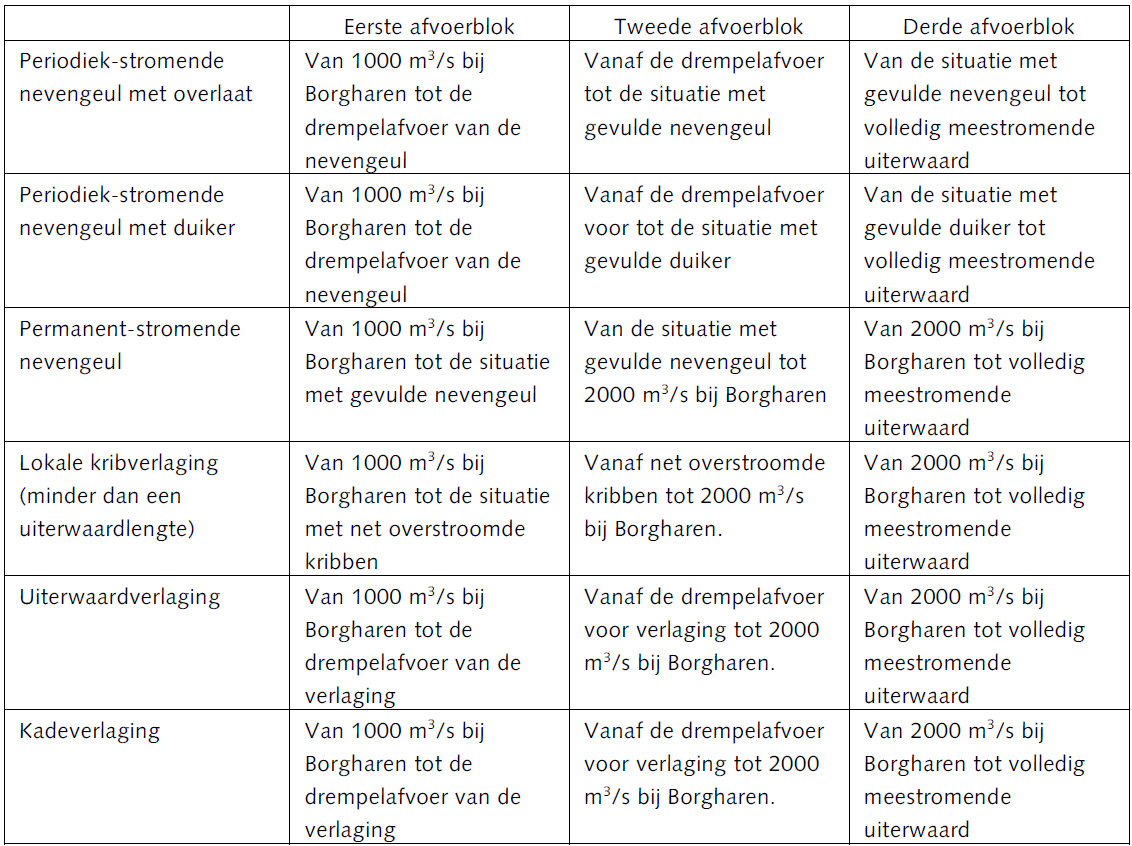
\includegraphics[width=\columnwidth]{figures/Tab1c.png}
\begin{tabular}{p{\columnwidth/4-12pt}|p{\columnwidth/4-12pt}|p{\columnwidth/4-12pt}|p{\columnwidth/4-12pt}}
 & first block & second block & third block \\ \hline
periodically flowing secondary channel with weir & from 1000 m\textsuperscript{3}/s at Borgharen to minimum discharge for secondary channel & from minimum discharge for secondary channel to bankfull secondary channel & from bankfull secondary channel to fully developed flood plain flow \\ \hline
periodically flowing secondary channel with orifice & from 1000 m\textsuperscript{3}/s at Borgharen to minimum discharge for secondary channel & from minimum discharge for secondary channel to fully flooded orifice & from fully flooded orifice to fully developed flood plain flow \\ \hline
permanently flowing secondary channel & from 1000 m\textsuperscript{3}/s at Borgharen to bankfull secondary channel & from bankfull secondary channel to 2000 m\textsuperscript{3}/s at Borgharen & from 2000 m\textsuperscript{3}/s at Borgharen to fully developed flood plain flow \\ \hline
local lowering of groynes (less than flood plain length) & from 1000 m\textsuperscript{3}/s at Borgharen to flooded groynes & from flooded groynes to 2000 m\textsuperscript{3}/s at Borgharen & from 2000 m\textsuperscript{3}/s at Borgharen to fully developed flood plain flow \\ \hline
lowering of the flood plain & from 1000 m\textsuperscript{3}/s at Borgharen to minimum discharge for new flood plain threshold & from new flood plain threshold to 2000 m\textsuperscript{3}/s at Borgharen & from 2000 m\textsuperscript{3}/s at Borgharen to fully developed flood plain flow \\ \hline
lowering of levees & from 1000 m\textsuperscript{3}/s at Borgharen to minimum discharge for new levee threshold & from new levee threshold to 2000 m\textsuperscript{3}/s at Borgharen & from 2000 m\textsuperscript{3}/s at Borgharen to fully developed flood plain flow \\
\end{tabular}

\caption{Overview of discharge conditions for various interventions along the Meuse.}
\label{App.Tab3}
\end{table}

\begin{figure}
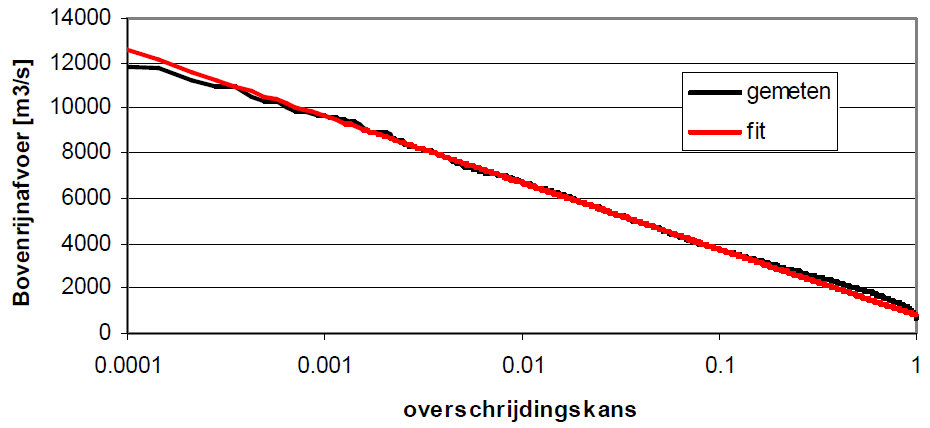
\includegraphics[width=\columnwidth]{figures/Fig3a.png}
\caption{Discharge exceedance curve for the Bovenrijn at Lobith (1970-2000).}
\label{App.Fig3a}
\end{figure}

\begin{figure}
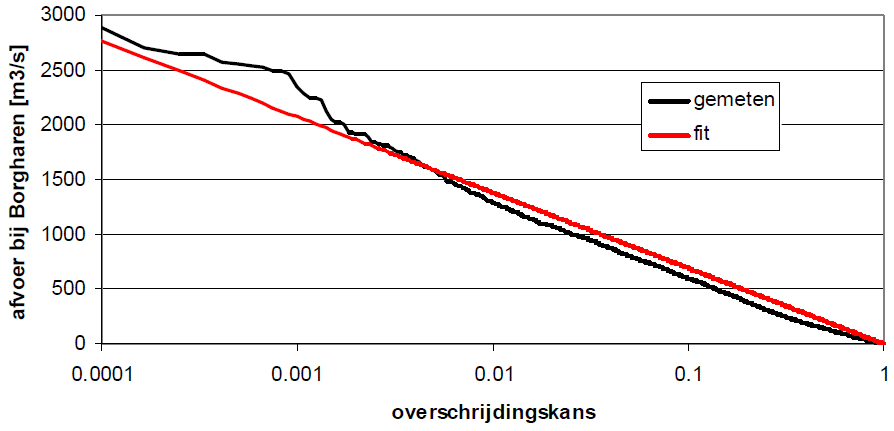
\includegraphics[width=\columnwidth]{figures/Fig3b.png}
\caption{Discharge exceedance curve for the Meuse at Borgharen (1975-2007).}
\label{App.Fig3b}
\end{figure}

In order to quickly estimate the yearly exceedance period for a given discharge, the discharge exceedance curve for the Bovenrijn has been approximated by a curve fitted through the observational data for the period 1970-2000 (\autoref{App.Fig3a}).
The number of days that the discharge $Q_\text{Bovenrijn}$ in the Bovenrijn at lobith is exceeded is given by

\begin{equation}
\label{Eq1a}
T_\text{exceedance, Bovenrijn} = 365 e^{\left ( \frac{800 -  Q_\text{Bovenrijn}}{1280} \right )}
\end{equation}

For the Meuse, in which --- due to imbrication (Grensmaas) and barriers (Zandmaas) --- the higher discharges are more important for the morphological development, the exceedance period for discharges at Borgharen can be estimated as

\begin{equation}
\label{Eq1b}
T_\text{exceedance, Meuse} = 365 e^{\left ( \frac{-  Q_\text{Borgharen}}{300} \right )}
\end{equation}

\subsection{Scientific background of the relaxation model for morphological change}

The rule-of-thumb used to determine the first estimate of the morphological effects within the main channel is based on a highly simplified model of the morphodynamics.
That model and the resulting rule-of-thumb are described in this section.

We start by assuming a quasi-stationary flow pattern and an outflow of discharge and sediment from the main channel while the local water level is independent of the hydraulic and morphological changes in the main channel (a \emph{rigid-lid} approximation).

\begin{figure}
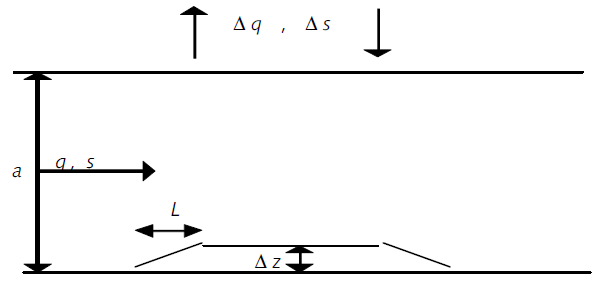
\includegraphics[width=\columnwidth]{figures/Fig4.png}
\caption{Schematic representation of the outflow of water and sediment}
\label{App.Fig4}
\end{figure}

The response of the main channel is represented here by a bed level change $\Delta z_b$ \unitbrackets{m} (raise or lowering) which is small relative to the local water depth.
The mass balance of the water and the sediment in the main channel can be written as
%
\begin{align}
&\text{water} & \pdiff{q_\text{mc}}{s} = -q_\text{out} \label{Eq2} \\
&\text{sediment} & \pdiff{z_b}{t} + \pdiff{s_\text{mc}}{s} = -s_\text{out} \label{Eq3}
\end{align}
%
in which
%
\begin{symbollist}
\item[$q_\text{mc}$] main channel unit discharge \unitbrackets{m\textsuperscript{2}/s}
\item[$q_\text{out}$] \emph{outflow of} unit discharge \emph{to} the flood plain per unit length \unitbrackets{m\textsuperscript{2}/sm}
\item[$s$] streamwise coordinate \unitbrackets{m}
\item[$z_b$] bed level change due to intervention \unitbrackets{m}
\item[$s_\text{mc}$] main channel unit sediment transport including pores \unitbrackets{m\textsuperscript{2}/s}
\item[$s_\text{out}$] \emph{outflow of} unit sediment transport including pores \emph{to} the flood plain per unit length \unitbrackets{m\textsuperscript{2}/sm}
\end{symbollist}

Note that the outflow of sediment is assumed to be a consequence of the outflow of discharge only; the conceptual framework does not allow for selective removal of only sediments.	
The unit sediment transport capacity in the main channel, $s_\text{mc}$, is approximated by $s_\text{mc} = m \left ( q_\text{mc} / h \right )^b$ with $h$ the water depth \unitbrackets{m} in the main channel, $m$ a dimensionless calibration factor and a dimensionless sediment transport exponent $b$ about 5 \citep{Engelundh67}.
Using this approximation the gradients in the sediment transport capacity can be written as
%
\begin{align}
\pdiff{s_\text{mc}}{s} &= m b \left ( \frac{q_\text{mc}}{h} \right )^{b-1} \pdiff{(q_\text{mc} / h)}{s} \\
&= m b \left ( \frac{q_\text{mc}}{h} \right )^{b-1} \left [ \frac{1}{h} \pdiff{q_\text{mc}}{s} - \frac{q_\text{mc}}{h^2} \pdiff{h}{s} \right ] \\
&= b \frac{s_\text{mc}}{q_\text{mc}} \pdiff{q_\text{mc}}{s} - b \frac{s_\text{mc}}{h} \pdiff{h}{s} \\
&\approx b \frac{s_\text{mc}}{q_\text{mc}} \pdiff{q_\text{mc}}{s} + b \frac{s_\text{mc}}{h} \pdiff{z_b}{s}
\label{Eq4}
\end{align}
%
if we assume that the water level gradient is negligible ($\pdiff{z_w}{s} \approx 0$) such that $\pdiff{h}{s} \approx -\pdiff{z_b}{s}$.
Substitution of \autoref{Eq4} into \autoref{Eq3} gives
%
\begin{equation}
\pdiff{z_b}{t} + b \frac{s_\text{mc}}{q_\text{mc}} \pdiff{q_\text{mc}}{s} + b \frac{s_\text{mc}}{h} \pdiff{z_b}{s} = -s_\text{out}
\label{Eq5a}
\end{equation}
%
which after substitution of \autoref{Eq2} in the second term becomes
%
\begin{equation}
\frac{h}{b s_\text{mc}} \pdiff{z_b}{t} + \pdiff{z_b}{s} = h \frac{q_\text{out}}{q_\text{mc}} - h \frac{s_\text{out}}{b s_\text{mc}}
\label{Eq5}
\end{equation}

The dynamic bed level changes will develop starting from the upstream end of the intervention.
The length $L$ over which this sedimentation occurs (i.e.~varies from 0 upstream to maximum amount $\Delta z_b$ downstream) corresponds to the reach over which discharge leaves the main channel and in which the flow pattern is adjusted by the reduced discharge as sketched in \autoref{App.Fig4}.
Hence, this length $L$ may thus be significantly shorter than the length of the intervention or the distance between the inflow and outflow openings of a secondary channel.
The integration of \autoref{Eq5} over this length $L$ results in a relaxation model for the dynamic bed level change due to the intervention
%
\begin{equation}
\frac{h}{b s_\text{mc}} \int_0^L \pdiff{z_b}{t} ds + \int_0^L \pdiff{z_b}{s} ds = \int_0^L \left [ h \frac{q_\text{out}}{q_\text{mc}} - h \frac{s_\text{out}}{b s_\text{mc}} \right ] ds
\label{Eq5a}
\end{equation}
%
\begin{equation}
\frac{h}{b s_\text{mc}} L^* \pdiff{\Delta z_b}{t} + \Delta z_b = - h \frac{\Delta q_\text{mc}}{q_\text{mc}} + h \frac{\Delta s_\text{mc}}{b s_\text{mc}}
\label{Eq5b}
\end{equation}
%
which $\Delta q_\text{mc}$ is the total change in unit discharge in the main channel due to the intervention \unitbrackets{m\textsuperscript{2}/s} and $\Delta s_\text{mc}$ is the total change in unit sediment transport due to the intervention \unitbrackets{m\textsuperscript{2}/s}.
Please note that $q_\text{out}$ was defined above positive for fluxes towards the flood plain, however, the resulting change $\Delta q_\text{mc}$ in the unit discharge within the main channel will be negative for such conditions (equivalently for $s_\text{out}$ and $\Delta s_\text{mc}$); this introduces a sign change on the right hand side.
%
\begin{equation}
\diff{\Delta z_b}{t} = \frac{\Delta z_{b,\text{eq}} - \Delta z_b}{T_m}
\label{Eq5dif}
\end{equation}
%
with a morphological time scale \unitbrackets{s}
%
\begin{equation}
T_m \approx \frac{h L}{b s_\text{mc}}
\label{Eq5T}
\end{equation}
%
and an equilibrium bed level change \unitbrackets{m} given by
%
\begin{equation}
\Delta z_{b,\text{eq}} = -h \left ( \frac{\Delta q_\text{mc}}{q_\text{mc}} - \frac{\Delta s_\text{mc}}{b s_\text{mc}} \right )
\label{Eq6}
\end{equation}
%
This relaxation behaviour can also be observed in the results of the numerical models (both 1D and 2D).

The rule-of-thumb is derived by posing that the bed level change $\Delta z_b$ can be interpreted as the bed level change due to an intervention over a distance $L$ along a stream line starting from the upstream end of the intervention.
The equilibrium value $\Delta z_{b,\text{eq}}$ depends according \autoref{Eq6} on the (original) water depth, the relative change in unit discharge and the relative change in the sediment transport.
The latter term is the result of the sediment flux into the secondary channel which dampens the effect of reduced sediment transport capacity in the main channel.
Ignoring this relatively minor dampening term results in a more conservative estimate.
For interventions over a short distance (i.e.~for the type of interventions for which the rule-of-thumb is applicable) the water level changes are an order of magnitude smaller than the bed level changes.
Therefore, one can rewrite \autoref{Eq6} to state that the equilibrium bed level change $\Delta z_{b,\text{eq}}$ equals the product of the water depth and the relative change in the main channel velocity $u$ \unitbrackets{m/s}:
%
\begin{equation}
\Delta z_{b,\text{eq}} \approx -h \left ( \frac{\Delta u}{u} \right )
\label{Eq6v2}
\end{equation}
%
A similar result can be obtained for graded bed material (sand/gravel mixtures) if it's assumed that the individual sediment fractions don't influence each other's mobility (Appendix C in \citet{Waterdienst2008}).
Such an assumption is valid at sufficiently high bed shear stresses, such as during flood conditions.

\subsection{The relaxation model applied to seasonal variability}

The bed level development during a relaxation period is (as a solution of \autoref{Eq5dif}) given by
%
\begin{equation}
z_{b,i} = z_{b,i} (0) + [z_{b,i,\text{eq}} - z_{b,i}(0)](1 - e^{-t/T_{m,i}})
\label{Eq7}
\end{equation}
%
with
%
\begin{symbollist}
\item[$z_{b,i}$] \unitbrackets{m} the morphological effect of the intervention during period $i$
\item[$z_{b,i}(0)$] \unitbrackets{m} the morphological effect at the start of period $i$
\item[$z_{b,i,\text{eq}}$] \unitbrackets{m} the equilibrium effect of the intervention during period $i$
\item[$t$] \unitbrackets{day} time
\item[$T_{m,i}$] \unitbrackets{day} the morphological time scale during period $i$
\end{symbollist}

\begin{figure}
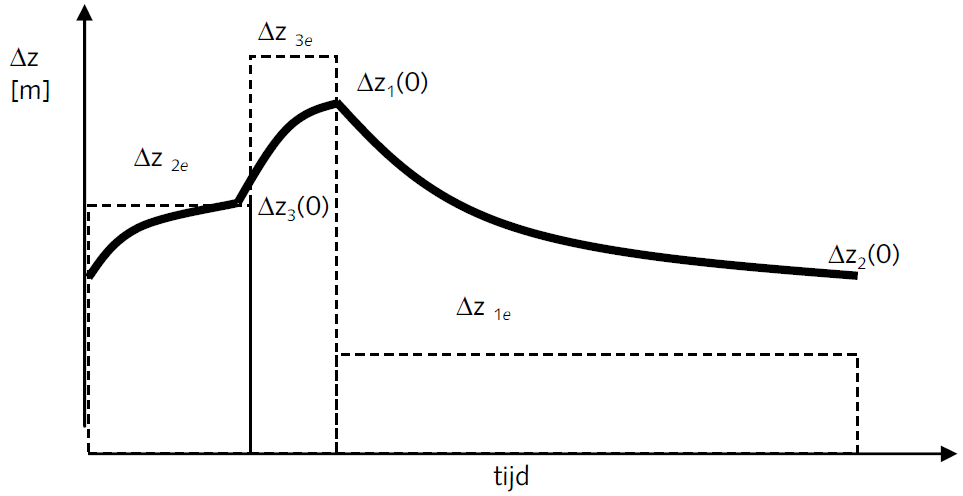
\includegraphics[width=\columnwidth]{figures/Fig5.png}
\caption{Schematic maximum bed level changes at the upstream end.}
\label{App.Fig5}
\end{figure}

\autoref{Eq7} implies that at the end of period $i$ (lasting for a period of $T_i$ days) the morphological effect of the intervention is given by
%
\begin{equation}
z_{b,i+1}(0) = z_{b,i} (0) \sigma_i + z_{b,i,\text{eq}} (1-\sigma_i) \text{ with } \sigma_i = e^{-T_i/T_{m,i}}
\label{Eq8a}
\end{equation}

If the yearly hydrograph is schematized using three periods, one obtains the following set of three equations for the three periods by assuming periodicity (the final bed level of the third period equals the initial bed level of the first period)
%
\begin{align}
z_{b,2}(0) &= z_{b,1}(0) \sigma_1 + z_{b,1,\text{eq}} (1-\sigma_1) \label{Eq8b} \\
z_{b,3}(0) &= z_{b,2}(0) \sigma_2 + z_{b,2,\text{eq}} (1-\sigma_2) \label{Eq8c} \\
z_{b,1}(0) &= z_{b,3}(0) \sigma_3 + z_{b,3,\text{eq}} (1-\sigma_3) \label{Eq8d}
\end{align}

We can solve these three equations for the unknown bed levels $z_{b,1}(0)$, $z_{b,2}(0)$ and $z_{b,3}(0)$.
This gives the following three expressions
%
\begin{align}
z_{b,1}(0) &= \frac{z_{b,1,\text{eq}} (1-\sigma_1) \sigma_2 \sigma_3 + z_{b,2,\text{eq}} (1-\sigma_2) \sigma_3 + z_{b,3,\text{eq}} (1-\sigma_3)}{1 - \sigma_1 \sigma_2 \sigma_3} \label{Eq8e} \\
z_{b,2}(0) &= \frac{z_{b,1,\text{eq}} (1-\sigma_1) + z_{b,2,\text{eq}} (1-\sigma_2) \sigma_3 \sigma_1 + z_{b,3,\text{eq}} (1-\sigma_3) \sigma_1}{1 - \sigma_1 \sigma_2 \sigma_3} \label{Eq8f} \\
z_{b,3}(0) &= \frac{z_{b,1,\text{eq}} (1-\sigma_1) \sigma_2 + z_{b,2,\text{eq}} (1-\sigma_2) + z_{b,3,\text{eq}} (1-\sigma_3) \sigma_1 \sigma_2}{1 - \sigma_1 \sigma_2 \sigma_3} \label{Eq8g}
\end{align}

The lower bound for the morphological impact of the intervention will be equal to $\min[z_{b,1}(0), z_{b,2}(0), z_{b,3}(0)]$ and the upper bound is given by $\max[z_{b,1}(0), z_{b,2}(0), z_{b,3}(0)]$.
For the schematized hydrograph shown in \autoref{App.Fig5} the bed level change is

\begin{itemize}
\item maximum at $z_{b,1}(0)$ (\autoref{Eq8e}) after flood period 3 (the third block in \autoref{App.Tab2})
\item minimum at $z_{b,2}(0)$ (\autoref{Eq8f}) after the low flow period 1 (the first block in \autoref{App.Tab2}).
\end{itemize}

In case the river section is experiences nearly stagnant flow conditions due to barriers a yearly period without bed level changes is inserted between low flow period 1 and the transitional flow period 2.\footnote{Earlier versions of this manual suggested that this period might be inserted between the flood period 3 and the low flow period 1, but algorithmically it was always placed between periods 1 and 2.}

We can't only obtain expressions for the two extreme (minimum, maximum) values but we can also determine an expression for the year-averaged bed level change by integrating \autoref{Eq7} per constant discharge period to
%
\begin{align}
\bar{z}_{b,i} &= \frac{1}{T_i} \int_0^{T_i}{z_{b,i} (0) + [z_{b,i,\text{eq}} - z_{b,i}(0)](1 - e^{-t/T_{m,i}})}dt \\
&= \frac{1}{T_i} \left . \left ( {z_{b,i,\text{eq}} t + [z_{b,i,\text{eq}} - z_{b,i}(0)]T_{m,i} e^{-t/T_{m,i}}} \right ) \right |_{t=0}^{t=T_i} \\
&= z_{b,i,\text{eq}} + [z_{b,i,\text{eq}} - z_{b,i}(0)] \frac{T_{m,i}}{T_i} ( e^{-T_i/T_{m,i}} - 1 )
\end{align}
%
and over all periods to
%
\begin{equation}
\bar{z}_b = \frac{\sum{z_{b,i,\text{eq}} T_i}}{\sum{T_i}} + \frac{\sum{(z_{b,i,\text{eq}}-z_{b,i}(0)) T_{m,i} (\sigma_i-1)}}{\sum{T_i}}
\label{Eq8h}
\end{equation}
%
If all bed level changes are removed after the flood period by means of dredging, the yearly dredging amount can finally be estimated by ignoring any excess depth.
After all, the maximum bed level change at the end of the flood season can with $z_{b,1}(0) = 0$ and \autoref{Eq8a} to \autoref{Eq8i} be expressed as the maximum dredging depth $z_\text{mdd}$

\begin{equation}
z_\text{mdd} = z_{b,1,\text{eq}}(1-\sigma_1) \sigma_2 \sigma_3 + z_{b,2,\text{eq}} (1-\sigma_2) \sigma_3 + z_{b,3,\text{eq}} (1-\sigma_3)
\label{Eq8i}
\end{equation}

Because this estimated doesn't take into account the sediment supply by the river, \autoref{Eq8i} can overestimate the maintenance dredging required.
\autoref{Eq8i} is therefore not included in the \dfastmi analysis.

\subsection{Estimate of the spatial distribution of the bed level changes}

\autoref{Eq8e} gives the maximum and \autoref{Eq8f} gives the minimum bed level change at the upstream end of the intervention.
Moving downstream for that point, the bed level change consists of a minimum bed level change $z_{b,1,\text{eq}}$ plus the part of the flood deposit that moves downstream during low flow conditions.
During a flood the downstream migrating sedimentation volume may temporarily even cause bed level changes larger than $z_{b,2,\text{eq}}$ but this is rather unlikely.
For convenience, it's therefore assumed that the maximum and minimum bed level change given by \autoref{Eq8e} and \autoref{Eq8f} are valid \emph{for each individual point in the main channel within the impacted area}.

This approximation implies that first the values of $z_{b,1,\text{eq}}$, $z_{b,2,\text{eq}}$ and $z_{b,3,\text{eq}}$ can be determined for every computational cell of the simulation in the main channel.
Subsequently the minimum (at the end of the low flow period) and maximum bed level change (at the end of the flood period) can be estimated given the approximated values for $\sigma_1$, $\sigma_2$ and $\sigma_3$ and \autoref{Eq8f} and \autoref{Eq8e} respectively.

\subsection{Time scales for bed level change}

The magnitude of the maximum bed level change at the end of the flood period and the minimum bed level change at the end of the low flow period both depend on the morphological time scales $T_{m,i}$ \unitbrackets{day} which define the rate of response of the bed levels.
Using \autoref{Eq5T} the time scale $T_{m,i}$ can also be written as $T_{m,i} = L/w_i$ with $w_i$ the bed celerity, i.e.~the propagation speed of bed level changes, and $L$ the distance intervention along the flow direction over which the bed level changes are accumulated.
As mentioned before, the length $L$ corresponds to the distance over which flow leaves the main channel and the flow pattern in the main channel adjusts to the reduced discharge.
Obviously, this distance varies in reality over the channel width and it depends on the discharge condition considered.
For consistent use of the rule-of-thumb, it's assumed that the length $L$ corresponds to twice the main channel width $B_\text{mc}$.

The second parameter in the definition of the morphological time scale is the bed celerity.
Based on statistics of width-averaged bed level observations averaged per km chainage year-averaged values have been determined \citep{RIZA2005} for the Dutch rivers.
These values are presented in \autoref{App.Tab2} and \autoref{App.Tab3} for Rhine branches and Meuse respectively.

\begin{table}
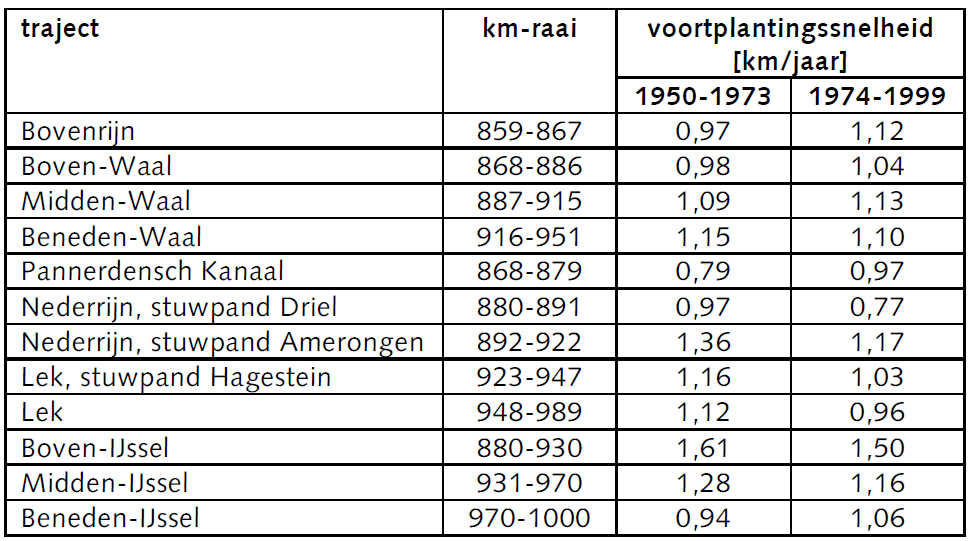
\includegraphics[width=\columnwidth]{figures/Tab2.png}
\caption{Overview of average bed celerities (based on km-averaged bed levels including the effects of dredging) by \citet{RIZA2005}.}
\label{App.Tab2Again}
\end{table}

\begin{table}
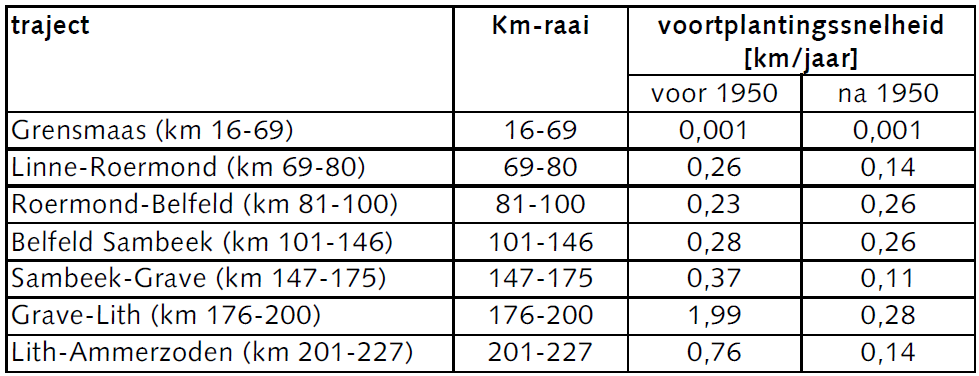
\includegraphics[width=\columnwidth]{figures/Tab3.png}
\caption{Overview of the reach averaged bed celerities (based on km-averaged bed levels including the effects of dredging) by \citet{Waterdienst2008}.}
\label{App.Tab3Again}
\end{table}

\begin{table}
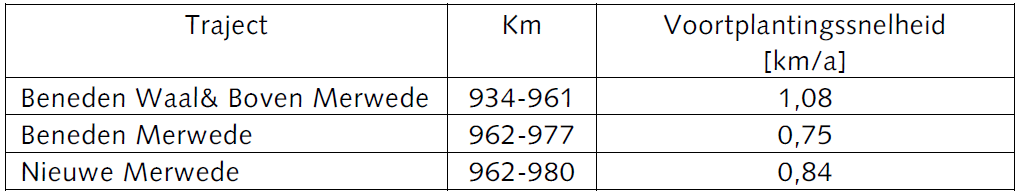
\includegraphics[width=\columnwidth]{figures/Tab4.png}
\caption{Overview of the reach averaged bed celerities (based on km-averaged bed levels for the period 1975-2000 including the effects of dredging) by \citet{RIZA2007}.}
\label{App.Tab4}
\end{table}

In order to translate these empirical year averaged values to discrete values per discharge block the following approximation is used for free flowing Rhine branches.
For the Bovenrijn discharges which are predominantly larger than 4000 m\textsuperscript{3}/s (during on average 8 \% of the year) a "high flow bed celerity" $w_h$ of 10 m/dag (3.65 km/yr) is used.

For discharge blocks which are predominantly below 4000 m\textsuperscript{3}/s a "low flow bed celerity" $w_l$ is used which is derived from the year-averaged bed celerity $\bar{c}$ as

\begin{equation}
w_l = \frac{\bar{c} - 0.082 \cdot 365}{0.918}
\label{Eq9}
\end{equation}

However, this approximation \autoref{Eq9} is only valid for the free flowing Rhine branches, hence it's for instance not valid for the Nederrijn where at low discharges the barriers are closed (\autoref{App.Fig6}).

\begin{figure}
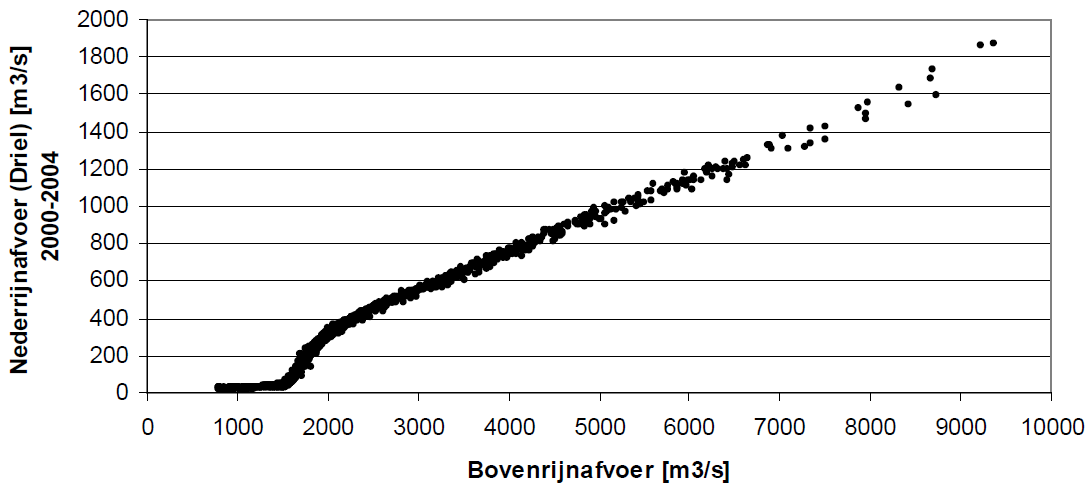
\includegraphics[width=\columnwidth]{figures/Fig6.png}
\caption{Nederrijn discharges at Driel-boven based on Donar database for the period 2000-2004).}
\label{App.Fig6}
\end{figure}

\autoref{App.Fig6} shows that the barriers in the Nederrijn are opened at a discharge of 1500 m\textsuperscript{3}/s in the Bovenrijn at Lobith (this value is exceeded during 57 \% of the year) and that the branch is approximately free flowing for discharges above 2200 m\textsuperscript{3}/s in the Bovenrijn at Lobith (exceeded during 33 \% of the year).
It's therefore assumed that the year-averaged bed celerity related to the low and high flow values as $\bar{c} = 0.082 w_h + (0.918 - 0.33) w_l$ such that for $w_h = 3,65$ km/yr we obtain

\begin{equation}
w_l = \frac{\bar{c} - 0.082 \cdot 3.65}{0.918 - 0.33}
\label{Eq10a}
\end{equation}

For the Meuse the we apply the following approximation.
It's assumed that the Meuse barriers are open for on average 10 days per year (3 \% of the time) such that the bed celerity can be estimated as

\begin{equation}
w_h = \frac{\bar{c}}{0.03}
\label{10b}
\end{equation}


Finally, due to the gradation the river bed of the Grensmaas will only become mobile at discharges above 1000 m\textsuperscript{3}/s which occurs on average about 4 days a year.
The bed celerity is thus estimated as

\begin{equation}
w_h = \frac{\bar{c}}{0.01}
\label{Eq10c}
\end{equation}

Based on the approximations \autoref{Eq9} to \autoref{Eq10c} and the year-averaged bed celerity values in \autoref{App.Tab2Again} to \autoref{App.Tab4} we obtain estimates for the bed celerities during high and low flow conditions.

\begin{table}
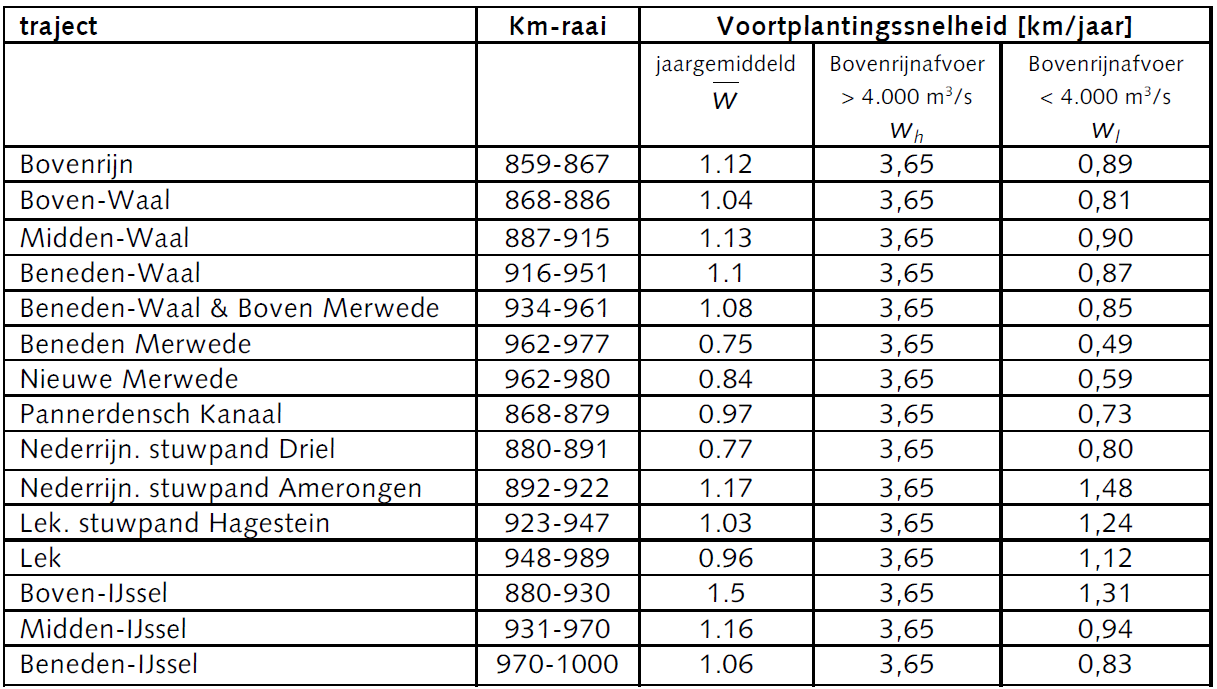
\includegraphics[width=\columnwidth]{figures/Tab4_the2nd.png}
\caption{Representative bed celerities during high- and low-flow conditions Rhine branches.}
\label{App.Tab4RT}
\end{table}

\begin{table}
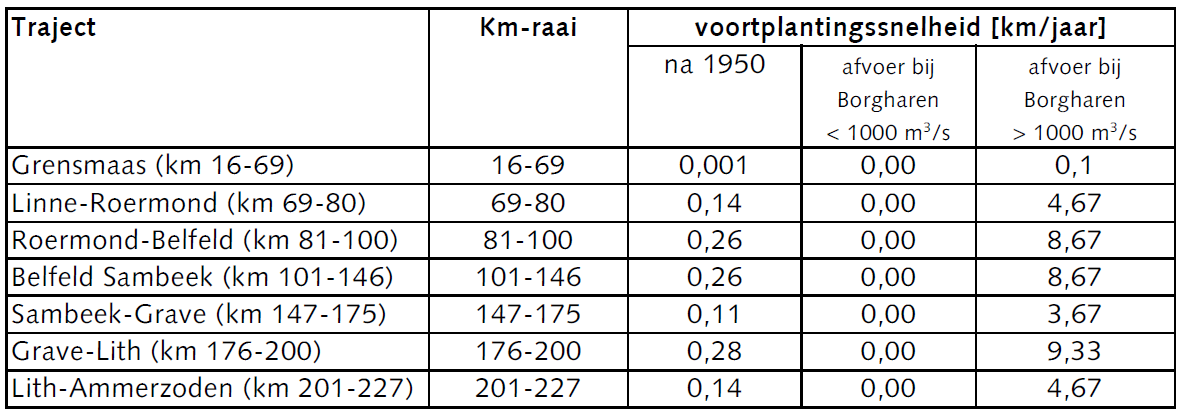
\includegraphics[width=\columnwidth]{figures/Tab5.png}
\caption{Representative bed celerities during high- and low-flow conditions Meuse.}
\label{App.Tab5}
\end{table}


\section{Steps in the analysis}

To apply the rule-of-thumb one should carry out the following five steps.
\dfastmi can perform steps 2 and 4 for you (except for the computation of $z_\text{mdd}$).

\begin{enumerate}
\item Characterize the intervention to be evaluated using \dfastmi

\begin{itemize}
\item Determine the threshold discharge $Q_\text{thr}$ (at Lobith/Borgharen) at which the intervention (indirectly) starts to influence the flow pattern in the main channel.

\item Determine the bankfull discharge $Q_\text{bf}$ (at Lobith/Borgharen) at which the intervention is fully flooded (bankfull flow)
\end{itemize}

\item Define the discharge blocks (block 1 "low flow", block 3 "flood" and block 2 "transitional between low and flood flows") using

\begin{itemize}
\item \autoref{App.Tab7} for the Rhine branches
\item \autoref{App.Tab8} for the Meuse
\end{itemize}

\item Perform the (up to six) necessary hydrodynamic simulations

\item Compute the characteristic bed level change per grid point in the main channel

\begin{itemize}
\item maximum value \unitbrackets{m} at the end of the flood season

\begin{equation}
z_{b,1}(0) = \frac{z_{b,1,\text{eq}} (1-\sigma_1) \sigma_2 \sigma_3 + z_{b,2,\text{eq}} (1-\sigma_2) \sigma_3 + z_{b,3,\text{eq}} (1-\sigma_3)}{1 - \sigma_1 \sigma_2 \sigma_3}
\end{equation}

\item minimum value \unitbrackets{m} at the end of the low flow season

\begin{equation}
z_{b,2}(0) = \frac{z_{b,1,\text{eq}} (1-\sigma_1) + z_{b,2,\text{eq}} (1-\sigma_2) \sigma_3 \sigma_1 + z_{b,3,\text{eq}} (1-\sigma_3) \sigma_1}{1 - \sigma_1 \sigma_2 \sigma_3}
\end{equation}

\item transitional value \unitbrackets{m} at the end of the transition block before the flood period

\begin{equation}
z_{b,3}(0) = \frac{z_{b,1,\text{eq}} (1-\sigma_1) \sigma_2 + z_{b,2,\text{eq}} (1-\sigma_2) + z_{b,3,\text{eq}} (1-\sigma_3) \sigma_1 \sigma_2}{1 - \sigma_1 \sigma_2 \sigma_3}
\end{equation}

\item year-averaged value \unitbrackets{m}

\begin{equation}
z_{b,m} = T_1 z_{b,1}(0) + T_2 z_{b,2}(0) + T_3 z_{b,3}(0)
\end{equation}

\item the maximum dredging depth (ignoring any excess depth)

\begin{equation}
z_\text{mdd} = z_{b,1,\text{eq}} (1-\sigma_1) \sigma_2 \sigma_3 + z_{b,2,\text{eq}} (1-\sigma_2) \sigma_3 + z_{b,3,\text{eq}} (1-\sigma_3)
\end{equation}
\end{itemize}

\item{Visualize the characteristic bed level changes in a graph or on a map}

\end{enumerate}

\begin{table}
\caption{Definition of discharge blocks for the Rhine branches}
\label{App.Tab7}
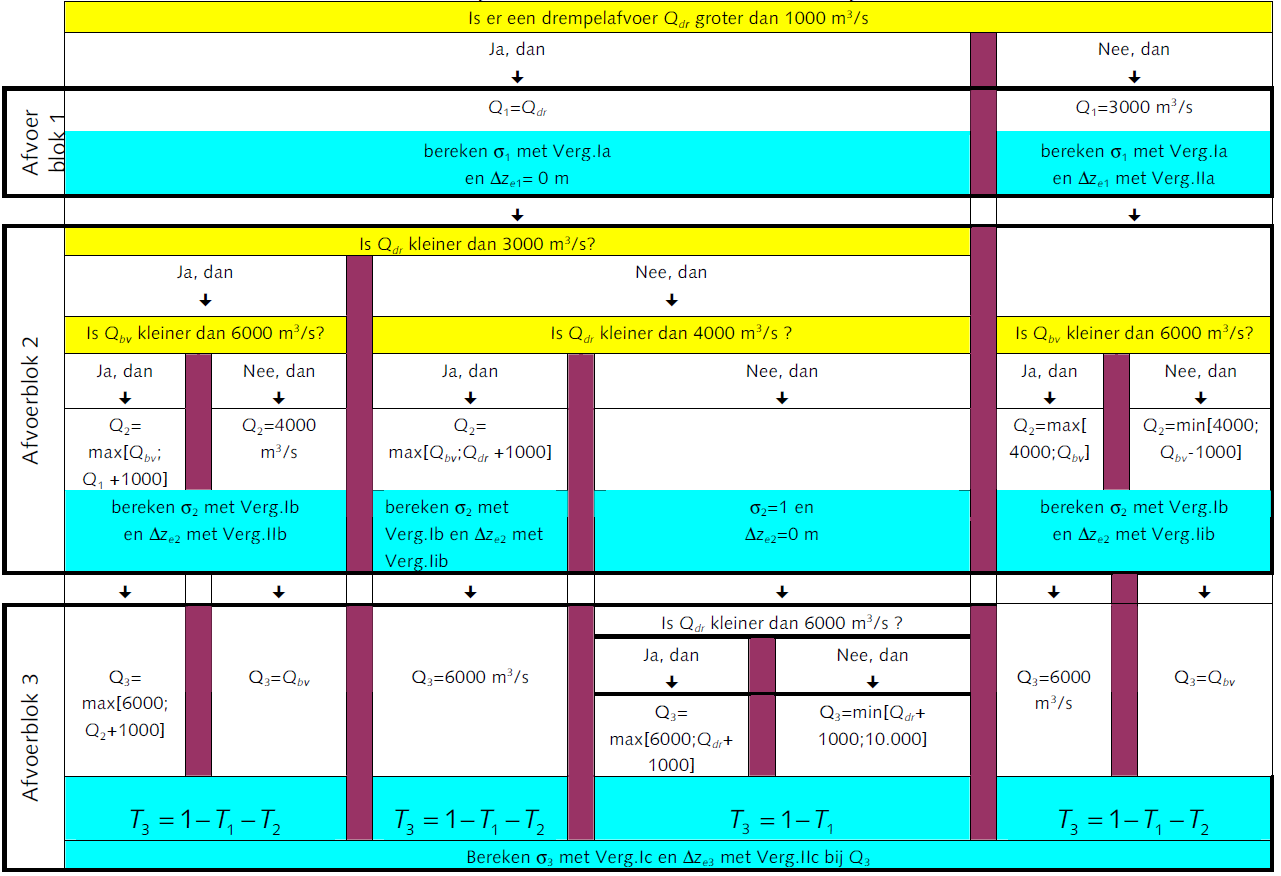
\includegraphics[width=\columnwidth]{figures/Tab7.png}
%
\begin{equation}
\sigma_1 = e^{-\frac{w_l}{2 B_n} T_1}
\end{equation}
with $T_1 = e^{\left ( \frac{800-Q_\text{bar}}{1280} \right )} - e^{\left ( \frac{800-Q_1}{1280} \right )}$ and $w_l$ from \autoref{App.Tab4RT} (with $Q_\text{bar} = 1500$ m\textsuperscript{3}/s for Nederrijn and Lek and $Q_\text{stuw} = 800$ m\textsuperscript{3}/s for the other branches)
%
\begin{equation}
\sigma_2 = e^{-\frac{w_h}{2 B_n} T_2}
\end{equation}
%
\begin{equation}
\sigma_3 = e^{-\frac{w_h}{2 B_n} T_3}
\end{equation}
with $T_2 = e^{\left ( \frac{800-Q_1}{1280} \right )} - e^{\left ( \frac{800-Q_2}{1280} \right )}$ and $w_h$ from \autoref{App.Tab4RT}.
%
\begin{equation}
\Delta z_{b,1,\text{eq}} = -h_o \frac{u_n - u_o}{u_o} \text{  for $Q_1$}
\end{equation}
%
\begin{equation}
\Delta z_{b,2,\text{eq}} = -h_o \frac{u_n - u_o}{u_o} \text{  for $Q_2$}
\end{equation}
%
\begin{equation}
\Delta z_{b,3,\text{eq}} = -h_o \frac{u_n - u_o}{u_o} \text{  for $Q_3$}
\end{equation}
based on reference water depths $h_o$ and velocities $u_o$ and modified velocities $u_n$ from the simulations.
\end{table}


\begin{table}
\caption{Definition of discharge blocks for the Meuse}
\label{App.Tab8}
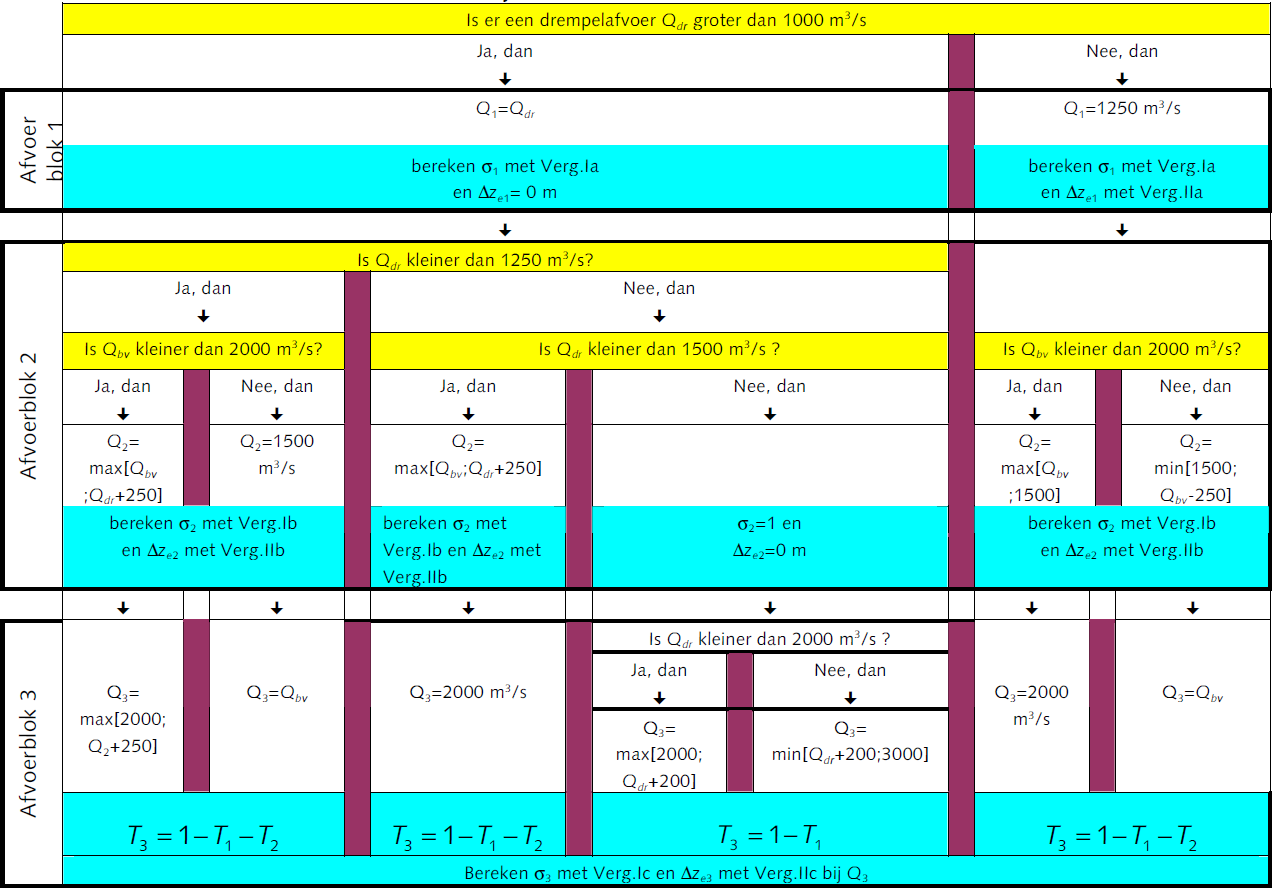
\includegraphics[width=\columnwidth]{figures/Tab8.png}
%
\begin{equation}
\sigma_1 = e^{-\frac{w_l}{2 B_n} T_1}
\end{equation}
with $T_1 = e^{\left ( - \frac{Q_\text{bar}}{300} \right )} - e^{\left ( - \frac{Q_1}{300} \right )}$; $Q_\text{bar} = 100$ m\textsuperscript{3}/s and $w_l$ from \autoref{App.Tab5}.
%
\begin{equation}
\sigma_2 = e^{-\frac{w_h}{2 B_n} T_2}
\end{equation}
%
\begin{equation}
\sigma_3 = e^{-\frac{w_h}{2 B_n} T_3} \text{ with $w_h$ from \autoref{App.Tab8}}
\end{equation}
 with $T_2 = e^{\left ( - \frac{Q_1}{300} \right )} - e^{\left ( - \frac{Q_2}{300} \right )}$ and $w_h$ from \autoref{App.Tab5}.
%
\begin{equation}
\Delta z_{b,1,\text{eq}} = -h_o \frac{u_n - u_o}{u_o} \text{  for $Q_1$}
\end{equation}
%
\begin{equation}
\Delta z_{b,2,\text{eq}} = -h_o \frac{u_n - u_o}{u_o} \text{  for $Q_2$}
\end{equation}
%
\begin{equation}
\Delta z_{b,3,\text{eq}} = -h_o \frac{u_n - u_o}{u_o} \text{  for $Q_3$}
\end{equation}
based on reference water depths $h_o$ and velocities $u_o$ and modified velocities $u_n$ from the simulations.

The premisses are: the flow in the main channel is well developed at $Q = 1000$ m\textsuperscript{3}/s, and at $Q = 2000$ m\textsuperscript{3}/s the flows in main channel and floodplain are both well developed.
\end{table}


\section{Examples}

This section describes three examples of how \dfastmi version 2 could be used.

\subsection{Example 1: secondary channel along the Waal}

For this (manually analyzed) case the effect of the secondary channel was analyzed by means of the results of a 1D \sobek model instead of 2D WAQUA or \dflowfm simulation results.
The secondary channel is located along the Waal river at chainage 900-905 km.
The secondary channel was represented in the 1D Rijntakken model as a local lateral extraction of river discharge.
The extraction was 3 \% of the total river discharge up to 4000 m\textsuperscript{3}/s beyond that the discharge increases linearly up to 10 \% at 7000 m\textsuperscript{3}/s and higher discharges.
The effect on the main channel discharge is shown for a number of characteristic cross-sectional profiles in \autoref{App.Fig7}.
The changes in the \emph{main channel} discharge caused by the secondary channel do not simply follow from the relationship between the secondary channel discharge and the \emph{total} river discharge.
After all, the secondary channel also lowers the water level which introduces a non-linear effect in particular in the lower range of the flood discharges.
As a result the \emph{main channel} discharge does not decrease proportionally to the extra flow area added by the secondary channel (e.g.~at the profile at km 900.5 at Bovenrijn discharges between 7000 and 8000 m\textsuperscript{3}/s).

\begin{figure}
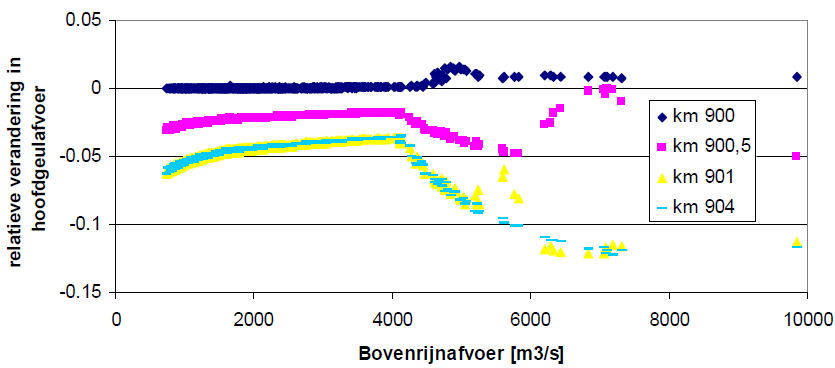
\includegraphics[width=\columnwidth]{figures/Fig7.png}
\caption{Influence of a secondary channel on the main channel discharge of the Waal}
\label{App.Fig7}
\end{figure}

\subsubsection*{Step 1) Characterize the intervention}

The secondary channel removes 3 \% of the total discharge for all discharges below 4000 m\textsuperscript{3}/s in the Bovenrijn.
Above that value the withdrawal increases linearly up to 10 \% at 7000 m\textsuperscript{3}/s.
There is no threshold discharge for the secondary channel: it is active at all discharges.
The secondary channel reaches bankfull at a river discharge of 4000 m\textsuperscript{3}/s.

\subsubsection*{Step 2) Define the discharge blocks}

Because there is no threshold discharge the discharge $Q_1 = 3000$ m\textsuperscript{3}/s is used for the first (low flow) block.
For the second block (transitional discharges) applies that the secondary channel reaches bankfull at 4000 m\textsuperscript{3}/s, so $Q_2 = 4000$ m\textsuperscript{3}/s.
The discharge $Q_3$ of the third block (flood) is in agreement with \autoref{App.Tab7} equal to 6000 m\textsuperscript{3}/s.
These values can be used to compute the relative duration of each block as

\begin{itemize}
\item $Q_1=3000$ m\textsuperscript{3}/s implies $T_1 = 1-e^{\frac{800-3000}{1280}} = 0.84$
\item $Q_2=4000$ m\textsuperscript{3}/s implies $T_2 = e^{\frac{800-3000}{1280}} - e^{\frac{800-4000}{1280}} = 0.09$
\item $Q_3=6000$ m\textsuperscript{3}/s implies $T_3 = 1-T_1-T_2 = 0.07$
\end{itemize}

\subsubsection*{Step 3) Equilibrium bed level changes}

For each of the three characteristic discharges the equilibrium bed level changes were determined for each relevant cross-sectional profile based on the \sobek results as

\begin{equation}
\Delta z_{b,i,\text{eq}} = -h_o \frac{Q_{\text{main channel},n} - Q_{\text{main channel},o}}{Q_{\text{main channel},o}}
\end{equation}

\Note Usually the results of a 2D model are used for each individual computational point in the main channel.
However, for this application based on \sobek results the total main channel discharge and the average main channel depth were used which thus only verifies the impact along a single stream path.

The resulting equilibrium values are shown in \autoref{App.Fig8}.

\begin{figure}
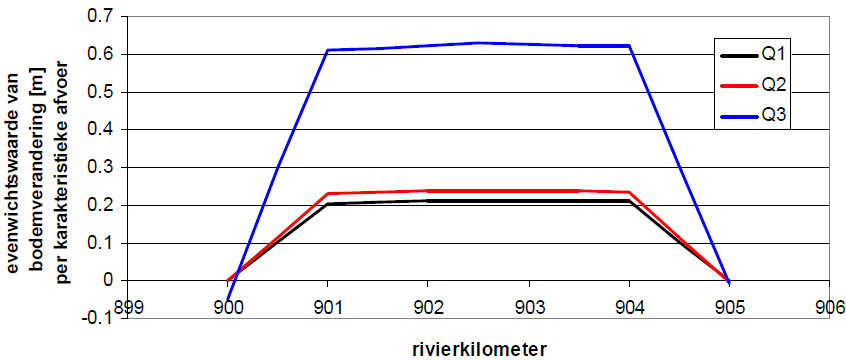
\includegraphics[width=\columnwidth]{figures/Fig8.png}
\caption{Equilibrium bed level changes in the main channel of the Waal at the site of the secondary channel.}
\label{App.Fig8}
\end{figure}

\subsubsection*{Step 4) Time scales for relaxation}

The main channel width (normal width between groyne heads) at the site of the secondary channel is 260 m.
The bed celerity for low discharges is 900 m/yr; for high discharges this increases to 3650 m/yr.
Consequently, for each block we can compute

\begin{align}
\sigma_1 &= e^{-\frac{w_l}{2B_n}T_1} = e^{-\frac{900}{2 \cdot 260} 0.84} = 0.18 \\
\sigma_2 &= e^{-\frac{w_l}{2B_n}T_2} = e^{-\frac{3650}{2 \cdot 260} 0.09} = 0.73 \\
\sigma_3 &= e^{-\frac{w_l}{2B_n}T_3} = e^{-\frac{3650}{2 \cdot 260} 0.07} = 0.78
\end{align}

\subsubsection*{Step 5) Computation of the characteristic bed level changes}

Based on the equilibrium values determined in step 3 and the relaxation factors of step 4 the characteristic bed level changes can be computed using

\begin{align}
z_{b,1}(0) &= \frac{z_{b,1,\text{eq}} (1-\sigma_1) \sigma_2 \sigma_3 + z_{b,2,\text{eq}} (1-\sigma_2) \sigma_3 + z_{b,3,\text{eq}} (1-\sigma_3)}{(1 - \sigma_1 \sigma_2 \sigma_3} \\
z_{b,2}(0) &= \frac{z_{b,1,\text{eq}} (1-\sigma_1) + z_{b,2,\text{eq}} (1-\sigma_2) \sigma_3 \sigma_1 + z_{b,3,\text{eq}} (1-\sigma_3) \sigma_1}{1 - \sigma_1 \sigma_2 \sigma_3}
\end{align}

To illustrate, the third characteristic bed level change has also been determined by means of
%
\begin{equation}
z_{b,3}(0) = \frac{z_{b,1,\text{eq}} (1-\sigma_1) \sigma_2 + z_{b,2,\text{eq}} (1-\sigma_2) + z_{b,3,\text{eq}} (1-\sigma_3) \sigma_1 \sigma_2}{1 - \sigma_1 \sigma_2 \sigma_3}
\end{equation}

For instance for cross-sectional profile km 901 we obtain $\Delta z_{b,1,\text{eq}} = 0.20$ m; $\Delta z_{b,2,\text{eq}} = 0.23$ m; $\Delta z_{b,3,\text{eq}} = 0.61$ m.
Substitution of these values into the aforementioned equations gives for km 901

\begin{align}
z_{b,1}(0) &= \tfrac{0.20 \cdot (1-0.18) \cdot 0.73 \cdot 0.78 + 0.23 \cdot (1-0.73) \cdot 0.78 + 0.61 \cdot (1-0.78)}{1 - 0.18 \cdot 0.73 \cdot 0.78} = 0.31 \\
z_{b,2}(0) &= \tfrac{0.20 \cdot (1-0.18) + 0.23 \cdot (1-0.73) \cdot 0.78 \cdot 0.18 + 0.61 \cdot (1-0.78) \cdot 0.18}{1 - 0.18 \cdot 0.73 \cdot 0.78} = 0.22 \\
z_{b,3}(0) &= \tfrac{0.20 \cdot (1-0.18) \cdot 0.73 + 0.23 \cdot (1-0.73) + 0.61 \cdot (1-0.78) \cdot 0.18 \cdot 0.73}{1 - 0.18 \cdot 0.73 \cdot 0.78} = 0.22
\end{align}

\subsubsection*{Step 6) Visualizing the results}

The alongstream profile of the characteristic bed level changes is shown together with the results obtained from \sobek in \autoref{App.Fig9}.
The $z_{b,1}(0)$ value (the characteristic maximum bed level change at the end of the flood period) corresponds in this case well with the bed level change that is not exceeded during 98 \% of the time.
the $z_{b,2}(0)$ value (the characteristic minimum bed level change at the end of the low flow period) corresponds in this case well with the bed level change which is not exceeded during 50 \% of the time.
The $z_{b,3}(0)$ value is in this particular case almost equal to $z_{b,2}(0)$ and it thus exceeds the simulated value that corresponds to the value not exceeded during 2 \% of the time.

\begin{figure}
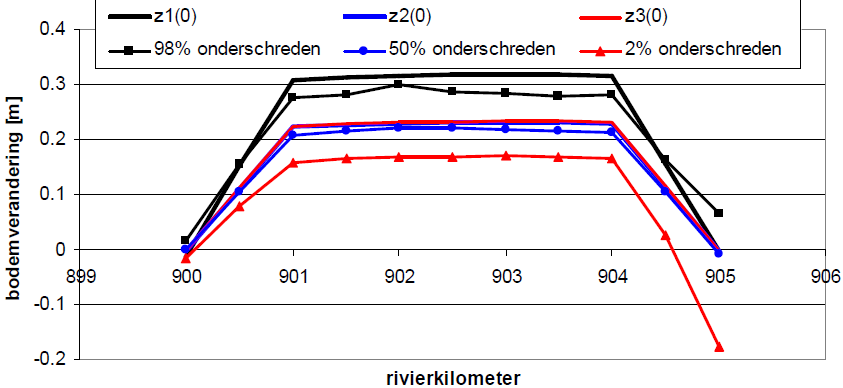
\includegraphics[width=\columnwidth]{figures/Fig9.png}
\caption{Estimated and simulated bed level changes at the secondary channel along the Waal.}
\label{App.Fig9}
\end{figure}

\subsection{Example 2: secondary channel along the Lek}

The second case also concerns a secondary channel; however, this time a secondary channel along the Lek between km 930 and km 935.
Also this secondary channel has been schematized as a local lateral extraction of flow from the overall river.
This extraction corresponds again to 3 \% of the total discharge for values up to 4000 m\textsuperscript{3}/s and increases linearly beyond to that 10 \% at 7000 m\textsuperscript{3}/s and higher discharges.
The effect on the main channel discharge is shown for a number of representative cross-sections in \autoref{App.Fig10}.

\begin{figure}
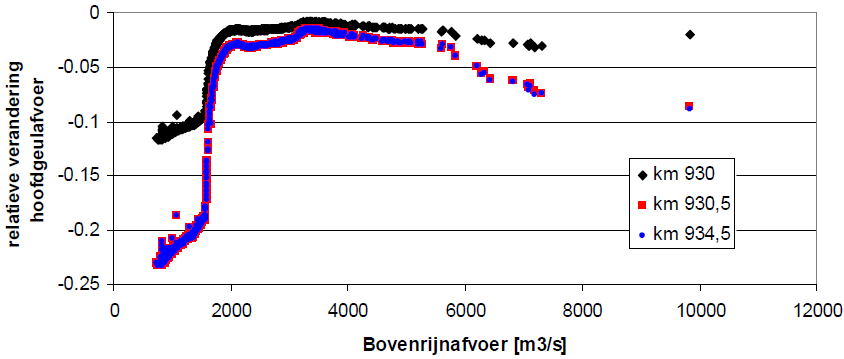
\includegraphics[width=\columnwidth]{figures/Fig10.png}
\caption{Influence of the secondary channel on the main channel discharge for the Lek}
\label{App.Fig10}
\end{figure}

\subsubsection*{Step 1) Characterize the intervention}

The secondary channel extracts 3 \% of the total discharge for Bovenrijn discharges up to 4000 m\textsuperscript{3}/s.
Above that value the withdrawal increases linearly up to 10 \% at 7000 m\textsuperscript{3}/s.
As in the first case there is no threshold discharge since the secondary channel is active for all discharges.
The reaches bankfull at a Bovenrijn discharge of 4000 m\textsuperscript{3}/s.

\subsubsection*{Step 2) Definition of the discharge blocks}

Because there is no threshold discharge the discharge $Q_1 = 1500$ m\textsuperscript{3}/s is used for the first (low flow) block.
For the second block (transitional discharges) applies that the secondary channel reaches bankfull at 4000 m\textsuperscript{3}/s, so $Q_2 = 4000$ m\textsuperscript{3}/s.
The discharge $Q_3$ of the third block (flood) is in agreement with \autoref{App.Tab7} equal to 6000 m\textsuperscript{3}/s.
These values can be used to compute the relative duration of each block as

\begin{itemize}
\item $Q_1=1500$ m\textsuperscript{3}/s implies $T_1 = 1-e^{\frac{800-1500}{1280}} = 0.42$
\item $Q_2=4000$ m\textsuperscript{3}/s implies $T_2 = e^{\frac{800-1500}{1280}} - e^{\frac{800-4000}{1280}} = 0.50$
\item $Q_3=6000$ m\textsuperscript{3}/s implies $T_3 = 1-T_1-T_2 = 0.08$
\end{itemize}

\subsubsection*{Step 3) Equilibrium bed level changes}

\begin{figure}
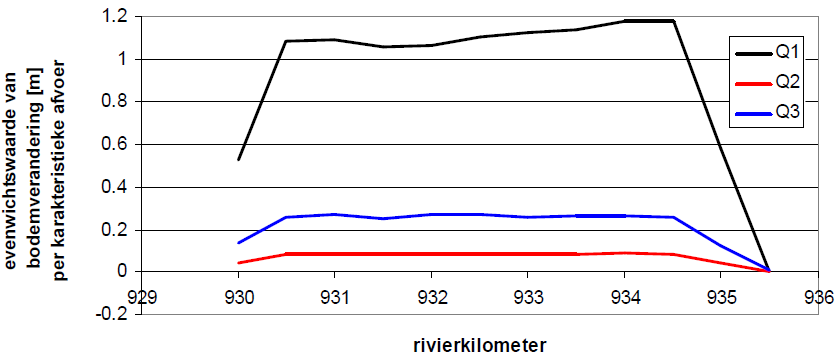
\includegraphics[width=\columnwidth]{figures/Fig11.png}
\caption{Equilibrium bed level changes in the main channel of the Lek at the site of the secondary channel.}
\label{App.Fig11}
\end{figure}

For each of the three characteristic discharges the equilibrium bed level changes were determined for each relevant cross-sectional profile based on the \sobek results as

\begin{equation}
\Delta z_{b,i,\text{eq}} = -h_o \frac{Q_{\text{main channel},n} - Q_{\text{main channel},o}}{Q_{\text{main channel},o}}
\end{equation}

\Note Usually the results of a 2D model are used for each individual computational point in the main channel.
However, for this application based on \sobek results the total main channel discharge and the average main channel depth were used which thus only verifies the impact along a single stream path.

The resulting equilibrium values are shown in \autoref{App.Fig11}.

\subsubsection*{Step 4) Time scales for relaxation}

The main channel width (normal width between groyne heads) at the site of the secondary channel is 140 m.
The bed celerity for low discharges is 0 m/yr; for high discharges this increases to 3120 m/yr.
Consequently, for each block we can compute

\begin{align}
\sigma_1 &= e^{-\frac{w_l}{2B_n}T_1} = e^{-\frac{0}{2 \cdot 140} 0.42} = 1.00 \\
\sigma_2 &= e^{-\frac{w_l}{2B_n}T_2} = e^{-\frac{3120}{2 \cdot 140} 0.50} = 0.004 \\
\sigma_3 &= e^{-\frac{w_l}{2B_n}T_3} = e^{-\frac{3120}{2 \cdot 140} 0.08} = 0.40
\end{align}

\subsubsection*{Step 5) Computation of the characteristic bed level changes}

Based on the equilibrium values determined in step 3 and the relaxation factors of step 4 the characteristic bed level changes can be computed.
For instance for cross-sectional profile km 930.5 we obtain $\Delta z_{b,1,\text{eq}} = 1.08$ m; $\Delta z_{b,2,\text{eq}} = 0.08$ m; $\Delta z_{b,3,\text{eq}} = 0.26$ m.
Substitution of these values into the appropriate equations gives for km 930.5

\begin{align}
z_{b,1}(0) &= \tfrac{1.08 \cdot (1-1.00) \cdot 0.004 \cdot 0.40 + 0.08 \cdot (1-0.004) \cdot 0.40 + 0.26 \cdot (1-0.40)}{1 - 1.00 \cdot 0.004 \cdot 0.40} = 0.20 \\
z_{b,2}(0) &= \tfrac{1.08 \cdot (1-1.00) + 0.08 \cdot (1-0.004) \cdot 0.40 \cdot 1.00 + 0.26 \cdot (1-0.40) \cdot 1.00}{1 - 1.00 \cdot 0.004 \cdot 0.40} = 0.20 \\
z_{b,3}(0) &= \tfrac{1.08 \cdot (1-1.00) \cdot 0.004 + 0.08 \cdot (1-0.004) + 0.26 \cdot (1-0.40) \cdot 1.00 \cdot 0.004}{1 - 1.00 \cdot 0.004 \cdot 0.40} = 0.08
\end{align}

\subsubsection*{Step 6) Visualizing the results}

\begin{figure}
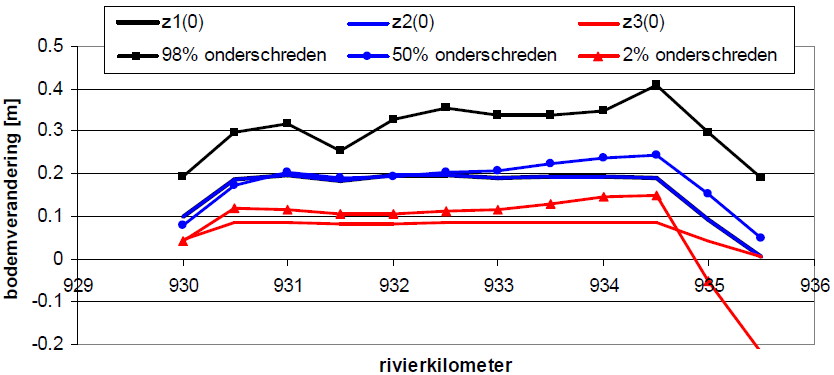
\includegraphics[width=\columnwidth]{figures/Fig12.png}
\caption{Estimated and simulated bed level changes at the secondary channel along the Lek.}
\label{App.Fig12}
\end{figure}

The alongstream profile of the characteristic bed level changes is shown together with the results obtained from \sobek in \autoref{App.Fig12}.
The $z_{b,1}(0)$ value (the characteristic maximum bed level change at the end of the flood period) corresponds in this case to the $z_{b,2}(0)$ value (the characteristic minimum bed level change at the end of the low flow period).
Both values correspond in this case well with the bed level change which is not exceeded during 50 \% of the time.
The $z_{b,3}(0)$ value corresponds in this particular case to the value not exceeded during 2 \% of the time.


\subsection{Example 3: an application to the Maas}

This example shows an analysis that was carried out using the original WAQMORF tool, but results of the latest \dfastmi program are consistent so it's still relevant.
The analysis was based on results obtained using the WAQUA model of "Over de Maas" of \citep{Svasek2007}.
The simulation results were provided by Ed Lemaire (DLB).

The test consisted of the following steps

\begin{enumerate}
\item The tool \dfastmi was used to determine the --- for the morphology --- representative discharges.
This step returned the discharges 1250 m\textsuperscript{3}/s, 1500 m\textsuperscript{3}/s and 2000 m\textsuperscript{3}/s at Borgharen.

\item WAQUA simulations were carried for both the reference situation and situation with the intervention implemented.
The water depths and flow velocities were exported using WAQVIEW to the export files supported by \dfastmi.

\item The export files were used as input for a second run of \dfastmi to estimate i) the mean annual bed level change, ii) the maximum bed level change (at the end of the flood season) and iii) the minimum bed level change (at the end of the low flow season)
\end{enumerate}

\begin{figure}
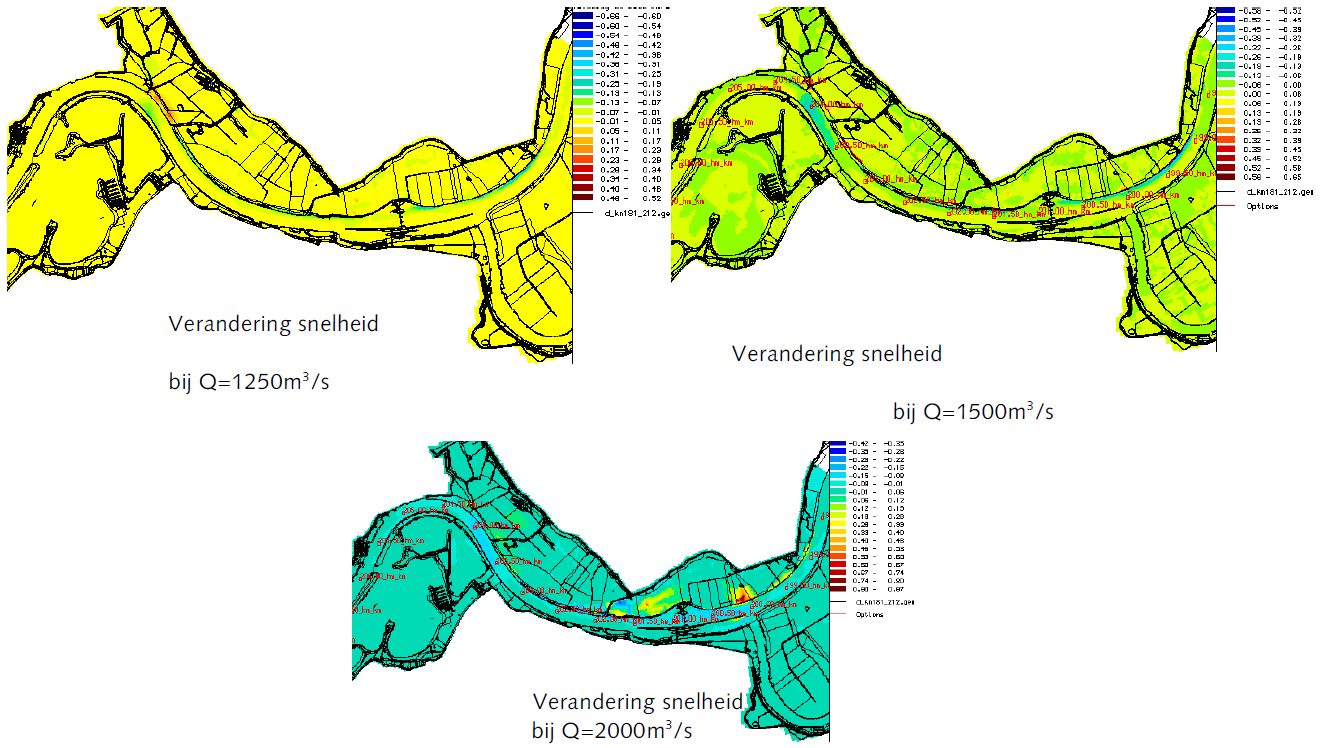
\includegraphics[width=\columnwidth]{figures/Fig13.png}
\caption{Overview of the velocity changes due to the intervention}
\label{App.Fig13}
\end{figure}

The biggest local bed level changes are located in the bend immediately downstream of the intervention.
The figures show the mean annual bed level changes in cm for three different critical velocities for the initiation of motion.
This parameter turns out to have little effect in this particular case.
The impact of the plan on river maintenance can be determined based on the available space in the navigation channel.

\begin{figure}
\center
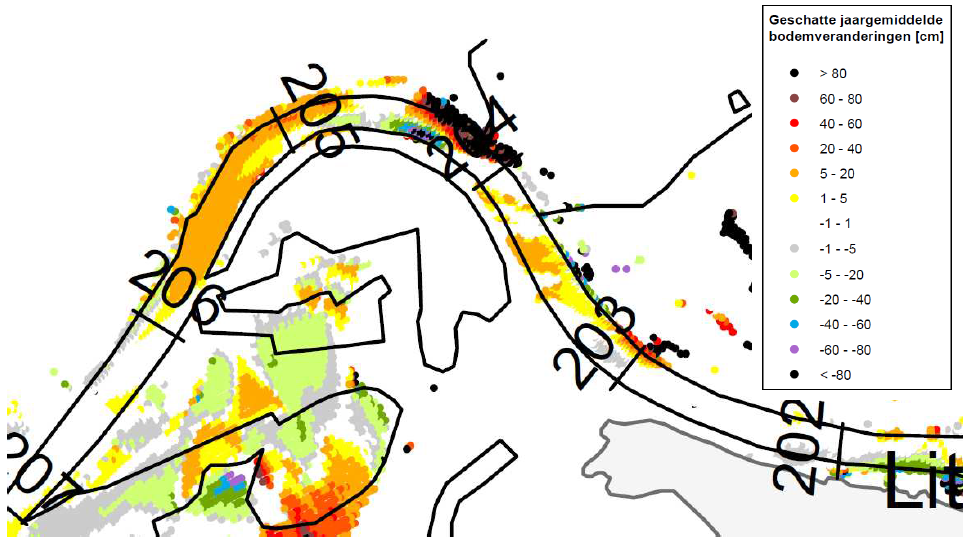
\includegraphics[width=12cm]{figures/Fig14a.png}
\caption{Estimated bed level changes (velocity threshold $u_{crit} = 0.01$ m/s).}
\label{App.Fig14a}
\end{figure}

\begin{figure}
\center
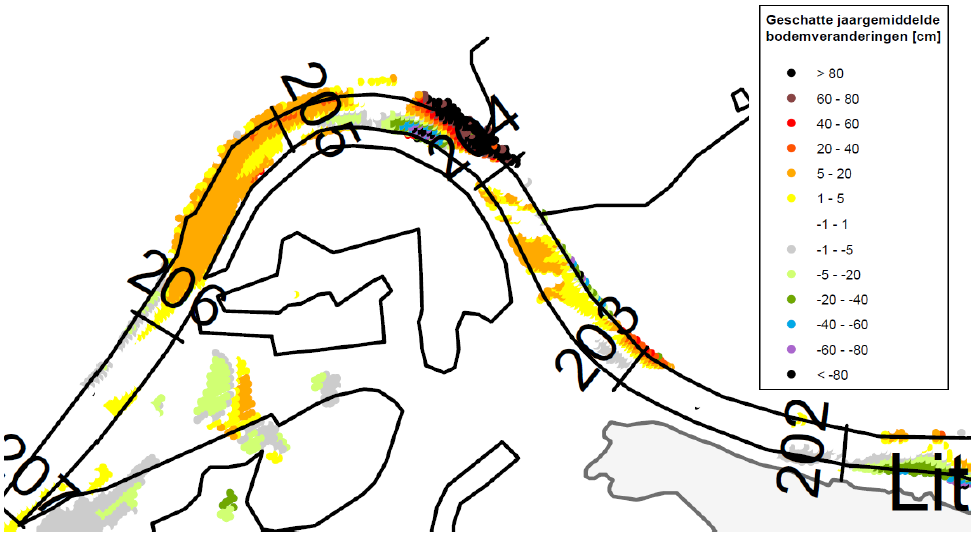
\includegraphics[width=12cm]{figures/Fig14b.png}
\caption{Estimated mean annual bed level changes (velocity threshold $u_{crit} = 0.10$ m/s).}
\label{App.Fig14b}
\end{figure}

\begin{figure}
\center
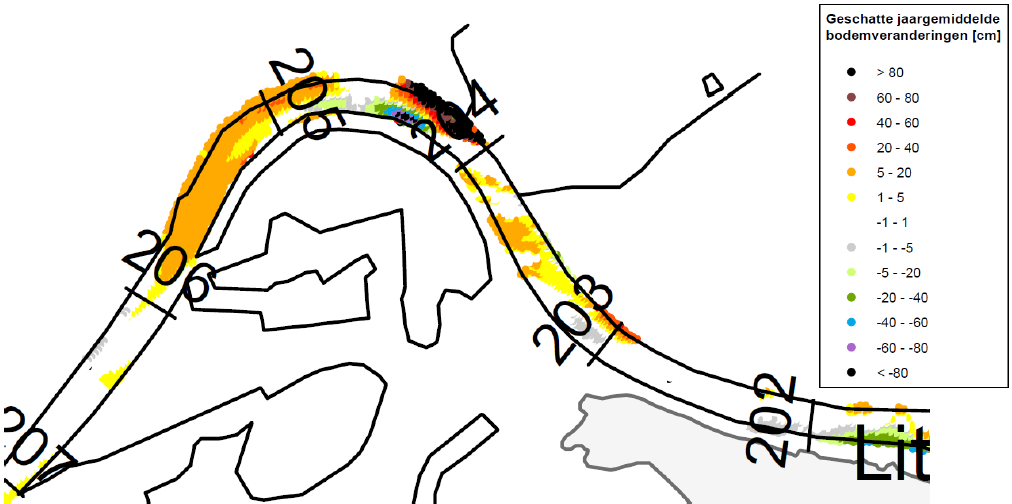
\includegraphics[width=12cm]{figures/Fig14c.png}
\caption{Estimated mean annual bed level changes (velocity threshold $u_{crit} = 0.30$ m/s).}
\label{App.Fig14c}
\end{figure}

\pagebreak[4]
\section{Example listing of the cli mode} \label{Sec:cli_dialog}

The following listing is an example of the interactive \keyw{cli} mode.

\begin{Verbatim}
This program implements the "WAQUA vuistregel" for the estimation of the local
morphological effects of a local intervention (i.e. an adjustment to the river). See
"RWS-WD memo WAQUA vuistregel 20-10-08" for details).

It is based on an estimation of the equilibrium bed level changes in the main
channel that would occur eventually when river maintenance would not be
adjusted.

The effect is expressed in [m] as:

    year-averaged bed level change without dredging
    maximum bed level change (after flood season) without dredging
    minimum bed level change (after low season) without dredging

By means of these estimates bottlenecks can be identified. The results are not
suitable for direct estimation of the impact on the maintenance of the
navigation channel!

The yearly sediment load of the river determines the period in which the
equilibrium can be reached.


This is version 3.0.0.

Confirm using "y" ...
\end{Verbatim}

You type \keyw{y}.

\begin{Verbatim}
The results are not valid for a combination of multiple interventions, or for a
single intervention extending over a distance more than 4 km!


In order to use D-FAST Morphological Impact you need to run reference and
scenario simulations on the same computational mesh.



The year discharge hydrograph is schematized using 3 blocks of constant
discharge:

    block 1 with discharge Q1 is the low water period
    block 2 with discharge Q2 is the transition period
    block 3 with discharge Q3 is the flood period


Are the simulation results already available?

Confirm using "y", or reply "n" ...
\end{Verbatim}

You type \keyw{y}.

\begin{Verbatim}
--------------------------------------------------------------------------------

The results of this program are three data files containing the characteristic
bed level changes. These files are:

    year-averaged change [m] without dredging in          "yearavg_dzb.out"
    maximum change [m] after flood without dredging in    "max_dzb.out"
    minimum change [m] after low flow without dredging in "min_dzb.out"

--------------------------------------------------------------------------------

Confirm using "y", or restart using "n" ...
\end{Verbatim}

You type \keyw{y}.

\begin{Verbatim}
On which branch is the intervention located?


    river branch                             nr

    Bovenrijn & Waal                         1

    Pannerdensch Kanaal & Nederrijn-Lek      2

    IJssel                                   3

    Merwedes                                 4

    Maas                                     5


The number of the river branch is ...
\end{Verbatim}

You type \keyw{1}.

\begin{Verbatim}
On which reach is the intervention located?


    river reach                             nr

    Bovenrijn                    km  859-867 1

    Boven-Waal                   km  868-886 2

    Midden-Waal                  km  887-915 3

    Beneden-Waal                 km  916-951 4


The number of the river reach is ...
\end{Verbatim}

You type \keyw{2}.

\begin{Verbatim}
--------------------------------------------------------------------------------

The intervention is located on reach Boven-Waal                   km  868-886

--------------------------------------------------------------------------------

Confirm using "y" or restart the location selection using "n" ...
\end{Verbatim}

You type \keyw{y}.

\begin{Verbatim}
The next three questions will be used to characterize the intervention. If an intervention
impacts the hydrodynamics in the main channel at multiple locations, answer the
questions for the part of the intervention that is expected to have the most impact
on the navigation channel.



Is the intervention flow-carrying for all discharges at Lobith above 1000 m3/s?

Confirm using "y", or reply "n" ...
\end{Verbatim}

You type \keyw{y}.

\begin{Verbatim}
Most of the flood plains become flow-carrying for discharges above 4000
m3/s. Is the intervention also bankfull for these discharges?

Confirm using "y", or reply "n" ...
\end{Verbatim}

You type \keyw{y}.

\begin{Verbatim}
Are the simulation results for Q1 = 3000.0  m3/s available?

Confirm using "y", or reply "n" ...
\end{Verbatim}

You type \keyw{y}.

\begin{Verbatim}
Are the simulation results for Q2 = 4000.0  m3/s available?

Confirm using "y", or reply "n" ...
\end{Verbatim}

You type \keyw{y}.

\begin{Verbatim}
Are the simulation results for Q3 = 6000.0  m3/s available?

Confirm using "y", or reply "n" ...
\end{Verbatim}

You type \keyw{y}.

\begin{Verbatim}
Below a certain velocity noo bed level changes occur.
The threshold value is set to  0.300000 m/s.

Is this an appropriate value for the reach Boven-Waal                   km  868-886?'

Confirm using "y", or reply "n" ...
\end{Verbatim}

You type \keyw{y}.

\begin{Verbatim}
Input of block 1 data files at Q=3000.0 m3/s

--------------------------------------------------------------------------------


The file name of flow velocity magnitudes without intervention is...
xyz_velocity-zeta.001.Q1.xyz
File "xyz_velocity-zeta.001.Q1.xyz" found!

The file name of water depths without intervention is...
xyz_waterdepth-zeta.001.Q1.xyz
File "xyz_waterdepth-zeta.001.Q1.xyz" found!

The file name of flow velocity magnitudes with intervention is...
xyz_velocity-zeta.002.Q1.xyz
File "xyz_velocity-zeta.002.Q1.xyz" found!

Reading the data files for block 1 ...


--------------------------------------------------------------------------------


Input of block 2 data files at Q=4000.0 m3/s

--------------------------------------------------------------------------------


The file name of flow velocity magnitudes without intervention is...
xyz_velocity-zeta.001.Q2.xyz
File "xyz_velocity-zeta.001.Q2.xyz" found!

The file name of water depths without intervention is...
xyz_waterdepth-zeta.001.Q2.xyz
File "xyz_waterdepth-zeta.001.Q2.xyz" found!

The file name of flow velocity magnitudes with intervention is...
xyz_velocity-zeta.002.Q2.xyz
File "xyz_velocity-zeta.002.Q2.xyz" found!

Reading the data files for block 2 ...


--------------------------------------------------------------------------------


Input of block 3 data files at Q=6000.0 m3/s

--------------------------------------------------------------------------------


The file name of flow velocity magnitudes without intervention is...
xyz_velocity-zeta.001.Q3.xyz
File "xyz_velocity-zeta.001.Q3.xyz" found!

The file name of water depths without intervention is...
xyz_waterdepth-zeta.001.Q3.xyz
File "xyz_waterdepth-zeta.001.Q3.xyz" found!

The file name of flow velocity magnitudes with intervention is...
xyz_velocity-zeta.002.Q3.xyz
File "xyz_velocity-zeta.002.Q3.xyz" found!

Reading the data files for block 3 ...


--------------------------------------------------------------------------------


Determining the characteristic bed level changes ...



If the bed level changes are removed on a yearly basis, the impacted river reach
is estimated at 1319 m from the upstream edge of the impacted reach.

Confirm using "y" to end the program ...
\end{Verbatim}

You type \keyw{y}.

\begin{Verbatim}
The program has ended !!!
\end{Verbatim}

\section{Old file formats}\label{app-v1:old-formats}

\subsection{Rivers configuration file}\label{app-v1:rivers}

The rivers configuration file follows the common ini-file format.
The file must contain a \keyw{[General]} block with a keyword \keyw{Version} to indicate the version number of the file.
The version number should be \keyw{1.0}.

Besides the \keyw{[General]} block version 1.0 files should only contain data blocks for the river branches (in Dutch: takken).
The names of those blocks will be used as branch names.
For instance, a block [My branch] will be processed as a branch called "My branch".
The order of the branches will correspond to the order of the blocks in the file.
The branch block defines the reaches (in Dutch: stukken) to be distinguished as well as the branch or reach specific parameter settings.
The \keyw{[General]} block may contain default values for the 
Further details follow below.

\begin{longtable}{l|l|p{8cm}}
\caption{Description of rivers configuration version 1} \\
Block & Keyword & Description \\ \hline
\endfirsthead
Block & Keyword & Description \\ \hline
      &         & \hfill\textsl{(continued from previous page)} \\ \hline
\endhead
      &         & \hfill\textsl{(continued on next page)} \\ \hline
\endfoot
\hline
\endlastfoot
\keyw{General} & \keyw{Version} & Version number. Must be \keyw{1.0}. \\
\keyw{General} & \keyw{Checksum} & Checksum of the rivers configuration file.
Used to verify whether the file wasn't accidentally modified. \\
BranchName<i> & \keyw{Reach<j>} & Name of reach <j> within branch <i> \\
BranchName<i> & \keyw{QLocation} & Location at which discharges for branch <i> are defined \\
\keyw{*} & \keyw{QStagnant} & Discharge \unitbrackets{m\textsuperscript{3}/s} below which main channel flow can be assumed stagnant \\
\keyw{*} & \keyw{QMin} & Minimum discharge \unitbrackets{m\textsuperscript{3}/s} at which intervention becomes active \\
\keyw{*} & \keyw{QFit} & Two discharges \unitbrackets{m\textsuperscript{3}/s} used for representing the exceedance curve \\
\keyw{*} & \keyw{QLevels} & Four characteristic discharges \unitbrackets{m\textsuperscript{3}/s} used by algorithm \\
\keyw{*} & \keyw{dQ} & Two discharge adjustments \unitbrackets{m\textsuperscript{3}/s} used by algorithm \\
\keyw{*} & \keyw{NWidth} & Normal width \unitbrackets{m} of main channel \\
\keyw{*} & \keyw{PRLow} & Low flow propagation rate \unitbrackets{km/yr} \\
\keyw{*} & \keyw{PRHigh} & High flow propagation rate \unitbrackets{km/yr} \\
\keyw{*} & \keyw{UCrit} & Critical (minimum) velocity \unitbrackets{m/s} for sediment transport
\end{longtable}

The second value of \keyw{QLevels} corresponds to the typical bankfull discharge.
All keywords listed for block \keyw{*} may occur either in the \keyw{[General]} block or in one of the branch specific blocks where they may optionally be concatenated with the reach number <j>.
Those keywords may thus occur in three flavours:

\begin{enumerate}
\item Plain keyword in block \keyw{[General]}: global default value valid for all branches
\item Plain keyword in branch specific block: default value for that branch (overrules any global default)
\item Keyword followed by reach number <j> in branch specific block: value valid for that reach on that branch.
\end{enumerate}

\subsubsection*{Example}

The following excerpt of the default \keyw{Dutch\_rivers.ini} configuration file shows the \keyw{[General]} as well as the first part of the \keyw{[Bovenrijn \& Waal]} block for the first branch.
It includes a global value of 0.3 for \keyw{UCrit} and 100 for \keyw{QMin}.
The other parameters are specified at branch level and mostly uniform for the whole branch.
Only \keyw{NWidth} and \keyw{PRLow} vary depending on the reach selected.

\begin{Verbatim}
    [General]
        Version    = 1.0

        UCrit      = 0.3
        QMin       = 1000

    [Bovenrijn & Waal]
        QLocation  = Lobith
        QStagnant  = 800
        QFit       = 800  1280
        QLevels    = 3000  4000  6000  10000
        dQ         = 1000  1000
        PRHigh     = 3.65
        
        Reach1     = Bovenrijn                    km  859-867
        NWidth1    = 340
        PRLow1     = 0.89
        
        Reach2     = Boven-Waal                   km  868-886
        NWidth2    = 260
        PRLow2     = 0.81

        ... continued ...
\end{Verbatim}

\subsection{Analysis configuration file}\label{app-v1:config}

The analysis configuration file follows the common ini-file format.
The file must contain a \keyw{[General]} block with a keyword \keyw{Version} to indicate the version number of the file.
The version number should be \keyw{1.0}.

Version 1.0 files must contain in the \keyw{[General]} block also the keywords \keyw{Branch} and \keyw{Reach} to identify the branch (in Dutch: tak) and reach (in Dutch: stuk) in which the intervention is located.
The specified names may be shortened, but they should uniquely identify the branch and reach amongst the names of the other branches and reaches.
Optionally, the same block may also contain \keyw{Qmin}, \keyw{QBankfull} and \keyw{UCrit} values representative for this particular intervention if they differ from those typical for the selected reach.
These items are sufficient for a basic analysis.
For a full spatial analysis the user needs to specify the names of the D-Flow FM map-files containing the results of the simulations without intervention (reference) and with intervention for the selected discharges Q1, Q2, and Q3.

\begin{tabular}{l|l|p{8cm}}
Block & Keyword & Description \\ \hline
\keyw{General} & \keyw{Version} & Version number. Must be \keyw{1.0}. \\
\keyw{General} & \keyw{Mode} & \keyw{WAQUA export} or \keyw{D-Flow FM map} (the latter is the default) \\
\keyw{General} & \keyw{Branch} & Name of the selected branch \\
\keyw{General} & \keyw{Reach} & Name of the selected reach \\
\keyw{General} & \keyw{QMin} & Minimum discharge \unitbrackets{m\textsuperscript{3}/s} at which intervention becomes active \\
\keyw{General} & \keyw{QBankfull} & Discharge \unitbrackets{m\textsuperscript{3}/s} at which intervention reaches bankfull \\
\keyw{General} & \keyw{UCrit} & Critical (minimum) velocity \unitbrackets{m/s} for sediment transport \\
\keyw{Q1} & \keyw{Discharge} & Discharge \unitbrackets{m\textsuperscript{3}/s} of the low flow simulation \\
\keyw{Q1} & \keyw{Reference} & Name of D-Flow FM map-file to be used for reference condition at Q1 \\
\keyw{Q1} & \keyw{WithMeasure} & Name of D-Flow FM map-file that includes the intervention at Q1 \\
\keyw{Q2} & \keyw{Discharge} & Discharge \unitbrackets{m\textsuperscript{3}/s} of the transitional regime \\
\keyw{Q2} & \keyw{Reference} & Name of D-Flow FM map-file to be used for reference condition at Q2 \\
\keyw{Q2} & \keyw{WithMeasure} & Name of D-Flow FM map-file that includes the intervention at Q2 \\
\keyw{Q3} & \keyw{Discharge} & Discharge \unitbrackets{m\textsuperscript{3}/s} of the high flow simulation \\
\keyw{Q3} & \keyw{Reference} & Name of D-Flow FM map-file to be used for reference condition at Q3 \\
\keyw{Q3} & \keyw{WithMeasure} & Name of D-Flow FM map-file that includes the intervention at Q3 \\
\end{tabular}

The file names may be specified using relative or absolute paths.
The \keyw{Reference} and \keyw{WithMeasure} keywords are *not* used when the \keyw{Mode} equals \keyw{WAQUA export}; in that case the file name are standardized as \keyw{xyz\_<quantity>-zeta.00<1/2>.Q<i>}.

\subsubsection*{Example}

This example shows a complete analysis configuration file for an intervention in the first branch/reach of the default \keyw{Dutch\_rivers.cfg} configuration.
It reports the default settings.
Only the \keyw{Version}, \keyw{Branch}, \keyw{Reach}, \keyw{Reference} and \keyw{WithMeasure} keywords are required for the full analysis.

\begin{Verbatim}
    [General]
      Version     = 1.0
      Mode        = D-Flow FM map
      Branch      = Bovenrijn & Waal
      Reach       = Bovenrijn                    km  859-867
      Qmin        = 1000.0
      Qbankfull   = 4000.0
      Ucrit       = 0.3
    
    [Q1]
      Discharge   = 1000.0
      Reference   = Measure42/Q1/Reference/DFM_OUTPUT_Q1/Q1_map.nc
      WithMeasure = Measure42/Q1/Updated/DFM_OUTPUT_Q1/Q1_map.nc
    
    [Q2]
      Discharge   = 4000.0
      Reference   = Measure42/Q2/Reference/DFM_OUTPUT_Q2/Q2_map.nc
      WithMeasure = Measure42/Q2/Updated/DFM_OUTPUT_Q2/Q2_map.nc
    
    [Q3]
      Discharge   = 6000.0
      Reference   = Measure42/Q3/Reference/DFM_OUTPUT_Q3/Q3_map.nc
      WithMeasure = Measure42/Q3/Updated/DFM_OUTPUT_Q3/Q3_map.nc
\end{Verbatim}


\section{Simulation result files}

The latest updates of \dfastmi only work using input data in UGRID netCDF files as obtained from \dflowfm.
Results obtained from Delft3D-FLOW and WAQUA can be converted to this format by means of \keyw{sim2ugrid}, a MATLAB-based conversion tool included in the QUICKPLOT distribution.

In backward compatibility mode, \dfmi can also read the same WAQUA files as used by WAQMORF.
The WAQUA simulation engine writes the simulation results in a proprietary SDS file format.
The content of these result files can't be accessed directly from Python, so they need to be exported to a more accessible file format.
The previous WAQMORF program also required that the user extracted the cell centred velocity magnitude and water depth values from the the WAQUA SDS-output files write them to simple ASCII files with 6 columns specifying the x-coordinates, y-coordinates, the value of the quantity (labeled as z-coordinate), m-index, n-index, and cell number.
Only the "z" values and the m- and n-indices are used by the program.
The names of those files has been hardcoded, they should read \keyw{xyz\_<quantity>-zeta.00<1/2>.Q<i>} with the quantity name equal to 'velocity' or 'waterdepth', a 1 for the reference simulation and a 2 for the simulation with the intervention implemented, and i the number of the discharge level.
\dfastmi supports these same files; an example of such file are given below.

\subsubsection*{Example}

\begin{Verbatim}
x,y,z,m,n,id
     197940.645,     431152.719,         0.0000,     2,     1,        11
     197874.004,     431430.516,         0.0000,     3,     1,        12
     197801.719,     431717.008,         0.0000,     4,     1,        13
     197727.047,     431985.375,         0.0000,     5,     1,        14
     197658.695,     432196.953,         0.0000,     6,     1,        15
     197610.234,     432323.859,         0.0000,     7,     1,        16
     197581.203,     432391.383,         0.0000,     8,     1,        17
     197559.625,     432439.234,         0.0000,     9,     1,        18
     197542.594,     432476.234,         0.0000,    10,     1,        19
     197528.668,     432506.070,         0.0000,    11,     1,        20
     197515.137,     432535.016,         0.0000,    12,     1,        21
     197505.176,     432556.258,         0.6156,    13,     1,        22
     197496.215,     432575.305,         0.8334,    14,     1,        23
     197485.773,     432597.516,         0.9794,    15,     1,        24
     197475.344,     432619.711,         1.0762,    16,     1,        25
     197465.578,     432640.484,         1.1305,    17,     1,        26
     197456.320,     432660.203,         1.1674,    18,     1,        27
     197447.242,     432679.563,         1.2085,    19,     1,        28
     197438.004,     432699.258,         1.2506,    20,     1,        29
     197428.273,     432720.000,         1.2913,    21,     1,        30
     197417.879,     432742.133,         1.3212,    22,     1,        31 

... continued ...
\end{Verbatim}


\subsection{Spatial output file}

The WAQMORF program wrote the spatial output in SIMONA BOX-file format which could be visualize when combined with the curvilinear grid of the original simulation.
\dfastmi still generates such files when run based on WAQUA results.


\pagestyle{empty}%
\cleardoublepage%
\mbox{}%

\includepdf[pages=2, offset=-72 -70]{cover/D-FAST-omslag-D-FAST Morphological Impact-TRN.pdf} % links-rechts past precies
\end{document}